% ---------------------------------------------------------------------------------
% Main tex file
% $Id: Thesis.tex,v 1.2 2012/02/04 22:54:40 matsch Exp $

\documentclass[
twoside=false,
headsepline,     % Line under page header
headings=normal,
open=any,
numbers=noenddot, % Otherwise there will be a dot after the chapter
numbering %in case letters are used somewhere e.g. in the appendix
]{scrreprt} %report scrreprt
\addtolength{\topmargin}{-0.2cm}
\setlength{\textwidth}{15cm}
\setlength{\textheight}{22.4cm}
%\oddsidemargin -0.2cm
%\evensidemargin 0.6cm



%\documentclass[
%a4,
%oneside,   %%% change here to twoside
%headsepline,     % Line under page header
%normalheadings,
%openany,
%numbers=noenddot % Otherwise there will be a dot after the chapter numbering in case letters are used somewhere e.g. in the appendix
%]{scrreprt} %report scrreprt
%\setlength{\textwidth}{15cm}
%\setlength{\textheight}{22.4cm}
%\oddsidemargin -0.1cm
%\evensidemargin 0.6cm

\usepackage[automark,headsepline]{scrpage2}

\pagestyle{scrheadings}
\clearscrheadfoot
\ihead{\headmark}
\ohead{\pagemark}
\cfoot{}
\setcounter{secnumdepth}{3}
\setcounter{tocdepth}{3}

% Alter some LaTeX defaults for better treatment of figures,
% from http://mintaka.sdsu.edu/GF/bibliog/latex/floats.html
% See p.105 of "TeX Unbound" for suggested values.
% See pp. 199-200 of Lamport's "LaTeX" book for details.
% General parameters, for ALL pages:
\renewcommand{\topfraction}{0.9}	% max fraction of floats at top
\renewcommand{\bottomfraction}{0.8}	% max fraction of floats at bottom
% Parameters for TEXT pages (not float pages):
%\setcounter{topnumber}{2}
%\setcounter{bottomnumber}{2}
%\setcounter{totalnumber}{4}     % 2 may work better
%\setcounter{dbltopnumber}{2}    % for 2-column pages
\renewcommand{\dbltopfraction}{0.9}	% fit big float above 2-col. text
\renewcommand{\textfraction}{0.07}	% allow minimal text w. figs
% Parameters for FLOAT pages (not text pages):
\renewcommand{\floatpagefraction}{0.7}	% require fuller float pages
% N.B.: floatpagefraction MUST be less than top fraction !!
\renewcommand{\dblfloatpagefraction}{0.7}	% require fuller float pages
% remember to use [htp] or [htpb] for placement

\newcommand{\wpj}{\ensuremath{\W\textrm{+jets}}\xspace}

\newcommand{\tbar}{\ensuremath{\bar{t}}\xspace}
\newcommand{\w}{\ensuremath{\W}}
\newcommand{\ptmiss}{\ensuremath{\slash\mkern-12mu{p}_{\text{T}}}\xspace} 
\newcommand{\pb}{\ensuremath{\pbinv}}

%% NUMBERS
\newcommand{\lumi}{\ensuremath{4.98 \xspace \fbinv}}
\newcommand{\dataPredi}{\ensuremath{453.5 \pm 53.4 \xspace}}
\newcommand{\mcPredi}{\ensuremath{542.1 \pm 5.0 \xspace}}


%special values forumlas etc.
%\newcommand\defMHT{\ensuremath{ {\rm MHT} = \mht = | - \sum_{i} \vec{p_{T} (jet_{i}) }|}}
%\newcommand{\mht}{\ensuremath{\slash\mkern-12mu{H}_{\text{T}}}\xspace}
%\newcommand{\MHT}{\mht}
%\newcommand{\jet}{\mathrm{jet}}
%\newcommand{\DeltaPhi}{\ensuremath{\Delta\phi_{\text{min}}}}

%\newcommand{\MET}{\ensuremath{\slash\mkern-12mu{M}_{\text{T}}}\xspace}
\newcommand{\mt}{\ensuremath{m_{T}}\xspace}

%\newcommand{\pt}{\ensuremath{p_{T}}}
%\newcommand{\phi}{$\Phi$}
%\newcommand{\tau}{$\tau$}
%\newcommand{\tau}{$\tau$}





\usepackage{amsfonts}
\usepackage{amsmath}  % Correct size switching in mathmode when using \text{} instead of \textrm{}
\usepackage{amssymb} 
\usepackage{amstext} 
\usepackage{multirow}
\usepackage{longtable}
\usepackage{cite}
\usepackage{graphicx}
\usepackage{booktabs}
\usepackage{tabularx}
\usepackage{multirow}
\usepackage{setspace}
\usepackage{rotating}


%%%%%%%%%%%% ALL chapters

%% definition of commands for latex
% ---------------------------------------------------------------------------------
% Collection of user-defined commands
% $Id: definitions.tex,v 1.3 2012/02/05 21:33:26 matsch Exp $

\usepackage{amsmath}
\usepackage{xspace}

\newcommand{\tobechecked}{\textcolor{red}{\textbf{(to be checked)}}}
\newcommand{\alreadydefined}[1]{\textcolor{red}{\textbf{(#1 already defined?)}}}
\newcommand{\todo}[1]{\textcolor{blue}{{\textbf{TODO: }\textit{#1}}}}
\newcommand{\fixme}[1]{\textcolor{red}{{\textbf{FIXME: }\textit{#1}}}}
\newcommand{\addref}{\textcolor{blue}{ADD REFERENCE}}
\newcommand{\addfig}[1]{\textcolor{red}{\textbf{ADD FIGURE: }\textit{#1}}}

% Sectioning
\newcommand{\qsec}[1]{Section~\ref{#1}}
\newcommand{\qsecs}[2]{Sections~\ref{#1} and~\ref{#2}}
\newcommand{\cfqsec}[1]{cf.\ Section~\ref{#1}}
\newcommand{\qfig}[1]{Fig.~\ref{#1}}
\newcommand{\qfigs}[2]{Figs.~\ref{#1} and~\ref{#2}}
\newcommand{\cfqfig}[1]{cf.\ Fig.~\ref{#1}}
\newcommand{\qsubfig}[2]{Fig.~\ref{#1}~(\textit{#2})}
\newcommand{\qtab}[1]{Table~\ref{#1}}
\newcommand{\qtabs}[2]{Tables~\ref{#1} and~\ref{#2}}
\newcommand{\cfqtab}[1]{cf.\ Table~\ref{#1}}
\newcommand{\qeq}[1]{\eqref{#1}}

% Units
\newcommand{\tev}{\ensuremath{\;\text{Te}\kern-0.06667em\text{V}}\xspace}
\newcommand{\gev}{\ensuremath{\;\text{Ge}\kern-0.06667em\text{V}}\xspace}
\newcommand{\mev}{\ensuremath{\;\text{Me}\kern-0.06667em\text{V}}\xspace}
\newcommand{\kev}{\ensuremath{\;\text{ke}\kern-0.06667em\text{V}}\xspace}
\newcommand{\ev}{\ensuremath{\;\text{e}\kern-0.06667em\text{V}}\xspace}
\newcommand{\tevnospace}{\ensuremath{\text{Te}\kern-0.06667em\text{V}}\xspace}
\newcommand{\gevnospace}{\ensuremath{\text{Ge}\kern-0.06667em\text{V}}\xspace}
\newcommand{\mevnospace}{\ensuremath{\text{Me}\kern-0.06667em\text{V}}\xspace}
\newcommand{\kevnospace}{\ensuremath{\text{ke}\kern-0.06667em\text{V}}\xspace}
\newcommand{\evnospace}{\ensuremath{\text{e}\kern-0.06667em\text{V}}\xspace}
\newcommand{\km}{\ensuremath{\;\text{km}}\xspace}
\newcommand{\m}{\ensuremath{\;\text{m}}\xspace}
\newcommand{\cm}{\ensuremath{\;\text{cm}}\xspace}
\newcommand{\mm}{\ensuremath{\;\text{mm}}\xspace}
\newcommand{\second}{\ensuremath{\;\text{s}}\xspace}
\newcommand{\kg}{\ensuremath{\;\text{kg}}\xspace}
\newcommand{\tons}{\ensuremath{\;\text{t}}\xspace}
\newcommand{\tesla}{\ensuremath{\;\text{T}}\xspace}
\newcommand{\kelvin}{\ensuremath{\;\text{K}}\xspace}
\newcommand{\nbinv}{\ensuremath{\;\text{nb}^{-1}}\xspace}
\newcommand{\pbinv}{\ensuremath{\;\text{pb}^{-1}}\xspace}
\newcommand{\fbinv}{\ensuremath{\;\text{fb}^{-1}}\xspace}

% Quantities
\newcommand{\et}{\ensuremath{E_{\text{T}}}\xspace}
\newcommand{\met}{\ensuremath{\slash\mkern-12mu{E}_{\text{T}}}\xspace}
\newcommand{\metvec}{\ensuremath{\slash\mkern-12mu{\vec{E}}_{\text{T}}}\xspace}
\newcommand{\HT}{\ensuremath{H_{\text{T}}}\xspace}
\newcommand{\HTvec}{\ensuremath{\vec{H}_{\text{T}}}\xspace}
\newcommand{\MHT}{\ensuremath{\slash\mkern-12mu{H}_{\text{T}}}\xspace}
\newcommand{\MHTvec}{\ensuremath{\slash\mkern-12mu{\vec{H}}_{\text{T}}}\xspace}
\newcommand{\pt}{\ensuremath{p_{\text{T}}}\xspace}
\newcommand{\ptvec}{\ensuremath{\vec{p}_{\text{T}}}\xspace}
\newcommand{\pti}[1]{\ensuremath{p_{\text{T},#1}}\xspace}
\newcommand{\ptivec}[1]{\ensuremath{\vec{p}_{\text{T},#1}}\xspace}
\newcommand{\ptsub}[1]{\ensuremath{p_{\text{T},#1}}\xspace}
\newcommand{\ptvecsub}[1]{\ensuremath{\vec{p}_{\text{T},#1}}\xspace}
\newcommand{\ptdijet}{\ensuremath{p^{\text{dijet}}_{\text{T}}}\xspace}
\newcommand{\ptave}{\ensuremath{p^{\text{ave}}_{\text{T}}}\xspace}
\newcommand{\ptavei}[1]{\ensuremath{p^{\text{ave}}_{\text{T,#1}}}\xspace}
\newcommand{\ptavemin}{\ensuremath{p^{\text{ave,min}}_{\text{T}}}\xspace}
\newcommand{\ptavemax}{\ensuremath{p^{\text{ave,max}}_{\text{T}}}\xspace}
\newcommand{\ptgen}{\ensuremath{p^{\text{gen}}_{\text{T}}}\xspace}
\newcommand{\ptgenave}{\ensuremath{p^{\text{gen,ave}}_{\text{T}}}\xspace}
\newcommand{\ptgenrel}{\ensuremath{p^{\text{gen,rel}}_{\text{T,3}}}\xspace}
\newcommand{\ptgeni}[1]{\ensuremath{p^{\text{gen}}_{\text{T},#1}}\xspace}
\newcommand{\ptgenivec}[1]{\ensuremath{\vec{p}^{\text{gen}}_{\text{T},#1}}\xspace}
\newcommand{\pthat}{\ensuremath{\hat{p}_{\text{T}}}\xspace}
\newcommand{\pthatmin}{\ensuremath{\hat{p}^{\text{min}}_{\text{T}}}\xspace}
\newcommand{\pthatmax}{\ensuremath{\hat{p}^{\text{max}}_{\text{T}}}\xspace}
\newcommand{\pttrue}{\ensuremath{p^{\text{true}_{}}_{\text{T}}}\xspace}
\newcommand{\pttruei}[1]{\ensuremath{p^{\text{true}_{}}_{\text{T,}#1}}\xspace}
\newcommand{\ptreco}{\ensuremath{p^{\text{reco}_{}}_{\text{T}}}\xspace}
\newcommand{\ptrel}{\ensuremath{p^{\text{rel}_{}}_{\text{T},3}}\xspace}
\newcommand{\ptmin}{\ensuremath{p^{\text{min}_{}}_{\text{T}}}\xspace}
\newcommand{\ptmax}{\ensuremath{p^{\text{max}_{}}_{\text{T}}}\xspace}
\newcommand{\ptparticle}{\ensuremath{p^{\text{particle}_{}}_{\text{T}}}\xspace}
\newcommand{\ptparton}{\ensuremath{p^{\text{parton}_{}}_{\text{T}}}\xspace}
\newcommand{\ptref}{\ensuremath{p^{\text{ref}_{}}_{\text{T}}}\xspace}
\newcommand{\ppgen}{\ensuremath{p^{\text{gen}}_{||}}\xspace}
\newcommand{\ppgeni}[1]{\ensuremath{p^{\text{gen}}_{||,#1}}\xspace}
\newcommand{\ppi}[1]{\ensuremath{p_{||,#1}}\xspace}
\newcommand{\ptimbal}{\ensuremath{p_{\text{T,imbal}}}\xspace}
\newcommand{\ptimbalrel}{\ensuremath{p^{\text{rel}}_{\text{T,imbal}}}\xspace}
\newcommand{\etamin}{\ensuremath{\eta^{\text{min}}}\xspace}
\newcommand{\etamax}{\ensuremath{\eta^{\text{max}}}\xspace}
\newcommand{\etagen}{\ensuremath{\eta^{\text{gen}}}\xspace}
\newcommand{\alphat}{\ensuremath{\alpha_{\text{T}}}\xspace}
\newcommand{\planckscl}{\ensuremath{\Lambda_{\text{P}}}\xspace}
\newcommand{\xtrue}{\ensuremath{x^{\text{true}}}\xspace}
\newcommand{\meanxtrue}{\ensuremath{\bar{x}^{\text{true}}}\xspace}
\newcommand{\xmeasi}[1]{\ensuremath{x_{#1}}\xspace}
\newcommand{\xave}{\ensuremath{x^{\text{ave}}}\xspace}

% Symbols
\newcommand{\dif}[1]{\ensuremath{\text{d}#1}\xspace}
\newcommand{\e}{\,\text{e}}
\newcommand{\nup}[1]{$^{\text{\scriptsize #1}}$}
\newcommand{\dgr}{\ensuremath{\,^{\circ}}}
\newcommand{\mean}[1]{\ensuremath{\langle#1\rangle}}
\newcommand{\gqq}[1]{\ensuremath{\glqq#1\grqq}}
\newcommand{\rarr}{\ensuremath{\rightarrow}\xspace}
\newcommand{\ket}[1]{\ensuremath{\left|#1\right>}\xspace}
\newcommand{\bra}[1]{\ensuremath{\left<#1\right|}\xspace}
\newcommand{\bracket}[2]{\ensuremath{\left<#2\right|#1\left|#2\right>}\xspace}

% Particles
\newcommand{\lel}{\ensuremath{e}\xspace}
\newcommand{\lelr}{\ensuremath{e_{R}}\xspace}
\newcommand{\lmu}{\ensuremath{\mu}\xspace}
\newcommand{\ltau}{\ensuremath{\tau}\xspace}
\newcommand{\nue}{\ensuremath{\nu_{e}}\xspace}
\newcommand{\nuer}{\ensuremath{\nu_{e,R}}\xspace}
\newcommand{\numu}{\ensuremath{\nu_{\mu}}\xspace}
\newcommand{\nutau}{\ensuremath{\nu_{\tau}}\xspace}
\newcommand{\qu}{\ensuremath{u}\xspace}
\newcommand{\qd}{\ensuremath{d}\xspace}
\newcommand{\qc}{\ensuremath{c}\xspace}
\newcommand{\qs}{\ensuremath{s}\xspace}
\newcommand{\qt}{\ensuremath{t}\xspace}
\newcommand{\qb}{\ensuremath{b}\xspace}
\newcommand{\photon}{\ensuremath{\gamma}\xspace}
\newcommand{\Z}{\ensuremath{Z^{0}}\xspace}
\newcommand{\W}{\ensuremath{W^{\pm}}\xspace}
\newcommand{\Wp}{\ensuremath{W^{+}}\xspace}
\newcommand{\Wm}{\ensuremath{W^{-}}\xspace}

% Processes
\newcommand{\ZInv}{\ensuremath{Z\rightarrow\nu\bar{\nu}}\xspace}
\newcommand{\ZInvJets}{\ZInv+jets\xspace}
\newcommand{\ttbar}{\ensuremath{t\bar{t}}\xspace}
\newcommand{\WJets}{\ensuremath{W}+jets\xspace}

% Programmes
\newcommand{\isajet}{\textsc{IsaJet}\xspace}
\newcommand{\madgraph}{\textsc{Madgraph}\xspace}
\newcommand{\prospino}{\textsc{Prospino}\xspace}
\newcommand{\pythia}{\textsc{Pythia}\xspace}
\newcommand{\herwig}{\textsc{Herwig++}\xspace}
\newcommand{\geant}{\textsc{GEANT4}\xspace}

% Experiments and facilities
\newcommand{\lhc}{LHC\xspace}
\newcommand{\cms}{CMS\xspace}
\newcommand{\dzero}{D\O\xspace}

% Other words and characters
\newcommand{\sm}{SM\xspace}
\newcommand{\susy}{SUSY\xspace}
\newcommand{\mssm}{MSSM\xspace}
\newcommand{\cmssm}{CMSSM\xspace}
\newcommand{\lsp}{LSP\xspace}
\newcommand{\dm}{DM\xspace}
\newcommand{\de}{DE\xspace}
\newcommand{\CLs}{\ensuremath{\text{CL}_{s}}\xspace}
\newcommand{\CL}{\ensuremath{\text{CL}}\xspace}
\newcommand{\cp}{CP\xspace}
\newcommand{\ratwo}{jets+met\xspace}
\newcommand{\hadtau}{hadronic-$\tau$\xspace}
\newcommand{\lostlep}{lost-lepton\xspace}
\newcommand{\PF}{PF\xspace}
\newcommand{\calo}{Calo jets\xspace}
\newcommand{\jpt}{JPT jets\xspace}
\newcommand{\pf}{PF jets\xspace}
\newcommand{\antikt}{anti-$k_{T}$\xspace}
\newcommand{\resp}{\ensuremath{\mathcal{R}}\xspace}
\newcommand{\asym}{\ensuremath{\mathcal{A}}\xspace}
\newcommand{\lvmini}{\textsc{LVMINI}\xspace}
\newcommand{\corescale}{\ensuremath{\lambda_{\text{res}}}\xspace}

% Symbols for tail studies
\newcommand{\fasym}{\ensuremath{f_{\text{asym}}}\xspace}
\newcommand{\fasymdata}{\ensuremath{f^{\text{data}}_{\text{asym}}}\xspace}
\newcommand{\fasymmc}{\ensuremath{f^{\text{mc}}_{\text{asym}}}\xspace}
\newcommand{\fasymtoy}{\ensuremath{f^{\text{toy}}_{\text{asym}}}\xspace}
\newcommand{\fresp}{\ensuremath{f_{\text{resp}}}\xspace}
\newcommand{\frespdata}{\ensuremath{f^{\text{data}}_{\text{resp}}}\xspace}
\newcommand{\frespmc}{\ensuremath{f^{\text{mc}}_{\text{resp}}}\xspace}
\newcommand{\fresptoy}{\ensuremath{f^{\text{toy}}_{\text{resp}}}\xspace}
\newcommand{\window}[1]{\ensuremath{>#1\,\sigma_{A}}}
\newcommand{\windowexcl}[2]{\ensuremath{#1-#2\,\sigma_{A}}}
\newcommand{\windowinf}[1]{\ensuremath{#1\,\sigma_{A} - \infty}}

% Abbrevations
\newcommand{\etc}{e.\,t.\,c.\ }
\newcommand{\wrt}{w.\,r.\,t.\ }
\newcommand{\cf}{cf.\ }
\newcommand{\ie}{i.\,e.\ }
\newcommand{\siehe}{s.\ }
\newcommand{\zb}{z.\,B.\ }
\newcommand{\ca}{ca.\ }
\newcommand{\eg}{e.\,g.\ }
\newcommand{\vs}{vs.\ }

% Constants
\newcommand{\lumiratwo}{\ensuremath{1.1\fbinv}\xspace}
\newcommand{\lumires}{\ensuremath{0.84\fbinv}\xspace}


%\title{Estimation of lost leptons from \ttbar and \wpj events at the CMS detector}
\author{Arne-Rasmus Dr\"ager}


%% config stuff
% pdflatex packages
\usepackage[pdftex]{hyperref}
\hypersetup{bookmarks=true}
\hypersetup{unicode=true}
\hypersetup{colorlinks=true,%
  citecolor=black,%
  filecolor=black,%
  linkcolor=black,%
  urlcolor=black}
\hypersetup{pdftitle={Search for Supersymmetry in All-Hadronic Final States at CMS}}
\hypersetup{pdfauthor={Arne-Rasmus Dr\"ager}}


%%%% start of the thesis

\begin{document}

%title page
\begin{titlepage}
  \begin{center}
    \thispagestyle{empty}
    \vspace*{1cm}
    \begin{doublespace} 
      \textbf{\huge
        Estimation of lost electrons and muons from \ttbar and \wpj events \linebreak
        at the CMS detector}\\
      \vskip1.5cm
      \begin{Large} 
        \textbf{Diplomarbeit\\
          Institute f\"{u}r Experimentalphysik\\
          der Universit\"{a}t Hamburg\\}
      \end{Large}
      \vskip2cm
      \begin{large}
        vorgelegt von\\
        {\bf Arne-Rasmus Dr\"{a}ger}
        \vfill
        \noindent{Hamburg\\2012}
      \end{large}
    \end{doublespace} 
  \end{center}
\end{titlepage}

\newpage
\thispagestyle{empty}

\quad
\vfill
\noindent{
\begin{tabular}{ll}
Gutachter der Doktorarbeit:                & Prof.\ Dr.\ Christian Sander\\ 

                                         
\end{tabular}
}

\newpage
\thispagestyle{empty}
\section*{Abstract}
The LHC has collected \lumi of proton-proton collisions at a center of mass energy of 7 TeV. A search for physics beyond the Standard Model with high energetic jets and large missing transverse energy takes advantage of this data. The background from Standard Model processes is estimated to a high precision using data-driven estimation methods. The prediction of the Standard Model background arising form \ttbar and \wpj events with unidentified electrons and muons from the involved \W-decay is presented in this thesis.\\
No excess above Standard Model expectation could be found. The results are interpreted within the minimal supersymmetric Standard Model and for Simplified Models excluding squark and qluino masses up to $\tilde q \approx 1.2$GeV and $\tilde g \approx 650$GeV. 
\clearpage
\section*{Abriss}
Der LHC hat \lumi von Proton-Proton Kollisionen bei einer Scherpunktsenergie von 7 TeV aufgezeichnet. Eine suche nach Physik jenseits des Standard Modells, mit hoch energetischen Jets und viel fehlender transversal Energie, wird in dieser Arbeit beschrieben. Untergrund von Standard Model Ereignissen wird mit einer hohen Pr\"{a}zision Daten-Getrieben vorher gesagt. Diese Arbeit beschreibt die Vorhersage von nicht detektiereten Muonen und Elektronen aus  \ttbar und \wpj Zerf\"{a}llen.\\
Es wird kein \"{U}berschuss an Ereignissen gegen\"{u}ber den vom Standard Modell erwarteten Ereignissen beobachtet. Das Resultat wird in dem minimal supersymmetric Standard Model und Simplified Models interpretiert. Massen von squark und qluino Massen unterhalb $\tilde q \approx 1.2$GeV und $\tilde g \approx 650$GeV k\"{o}nnen ausgeschlossen werden.
\newpage 
\thispagestyle{empty}
\quad 
\newpage

\pagenumbering{roman}
\setcounter{page}{1}
\tableofcontents

\cleardoublepage

\pagenumbering{arabic}
\setcounter{page}{1}





%\maketitle
\listoffigures
\chapter{Introduction}
\label{sec:introduction}
The Standard Model (SM) of particle physics is one of the most successful scientific theories. It has been extraordinary successful, not only in describing observed interactions and the production of particles, but also predicting new particles.\\
Build on gauge groups, the SM has shown its predictive power to a high precision, especially in electroweak processes, which have been tested at LEP to a very high accuracy.
The prediction and later discovery of the $W^{\pm},Z$ boson, which mediate the weak force, and of the $b$ and $t$ quarks has further increased the credency in the Standard Model. Despite all successes, experimental and theoretical arguments suggest that the Standard Model can only be consider a low energy approximation of a more fundamental theory.\\
For example Supersymmetry is able to solve many problems of the Standard Model in an elegant and convenient way. One prediction of Supersymmetric models is the existence of new massive particles. Interpretation of experimental results and phenomenological arguments suggest particle masses around the TeV scale, placing them in reach of the Large Hadron Colliders (LHC).\\
One of the main goals of the LHC and its two main experiments ATLAS and CMS is the search for these non SM particles. This thesis describes a search for such particles in events with jets and missing transverse momentum at CMS. Evidently it is crucial to predict the rate of such events due to Standard Model processes such as the production and decay of \W bosons.
The main focus of this thesis therefore is on one of the background estimation methods used to predict SM events involving not identified electrons and muons originating from \W decays leading to such a signature. The sum of the SM background estimations contributing to this analysis, is compared to observed events in the luminosity of \lumi collected by CMS in 2011. No excess over the Standard Model expectation has been found. The obtained exclusion limits are among the most sensitive limits on SUSY up to date.\\
This thesis starts with a short introduction to the Standard Model and Supersymmetry (Sec.~\ref{sec:theory}) followed by a description of the LHC and the CMS detector and its components (Sec.~\ref{sec:detector}). Next the concept of jets with missing transverse momentum analysis is introduced (Sec.~\ref{sec:search_beyondSM}) followed by a detailed discussion of the lost-lepton method (Sec.~\ref{sec:lostlepton}). The last part describes the other contributing background estimations, closing with the interpretation of the results within the cMSSM and Simplified Models (Sec.~\ref{sec:ra2}).

\cleardoublepage

\chapter{Theory}
\label{sec:theory}
\section{Standard Model}
\label{sec:SM}
%All known fundamental particles and forces can be describe by the standard model (SM). Only gravity is not included in the SM.
%One of the greatest success is that the SM was capable of predicting particles like the top quark before they were discovered.
%Since its development many experiments have performed precision measurements and up to now no deviation has been found.
%However there are some unresolved problems.
%This section describes the fundamental forces along with all particles and explains briefly the Higgs mechanism which is needed for particles to gather mass and generate the electroweak symmetry breaking.


During the 20th century the Standard Model of particle physics (SM) has been developed.  
The SM is a quantum field theory based on gauge invariance including all fundamental particles, leptons and quarks, and three fundamental forces, Quantum Chromodynamics (QCD)(Sec.~\ref{sec:qcd}) and Quantum Electrodynamics (QED)(Sec.~\ref{sec:qed}) unified with the weak force to the electro-weak force (Sec.~\ref{sec:electro-weak}). In addition the Higgs mechanism (Sec.~\ref{sec:higgs}) is introduced in order to generate masses for the weak gauge bosons and all fermions.% The interactions are introduced via three gauge symmetry groups (Sec. \ref{sec:gauge}).\\
Except for the Higgs-boson all particles and forces have been found experimentally. However, new LHC and Tevatron results have found consistently candidate events for a Higgs-boson with a mass of about 126 GeV\cite{ATLAS-CONF-2012-019}\cite{CMS-PAS-HIG-12-008}\cite{bib:TevatronHiggs:2011cb}. \\
This section covers a short introduction to gauge theory and the Dirac equation followed by the derivation of Quantum Electrodynamics (QED) from gauge theory and a phenomenological description of the strong force (QCD), the weak force and its unification with QED. Also the concept of the Higgs mechanism is briefly described. The last part covers some of the unresolved problems within the SM suggesting a more fundamental theory. 

%The SM can only be seen as a low energy approximation of a more fundamental theory
%re strong reasons why the SM can not be seen as a complete theory but only a low energy approximation of a more fundamental theory.\\ 


%Particles physics focuses on the investigation and explanation of the smallest constituents of matter and how they interact. The aim is to understand how the world around us is formed and what keeps it together on smallest scales.\\
%During the 20th century the so called Standard Model of Particle Physics (SM), has been developed. The SM consists of the basic ingredients of matter, leptons and quarks (see sec.\ref{subsec:fundamental_particles}) and the fundamental forces, the quantum chromodynamics (sec. \ref{sec:qcd}) the electro-weak force (sec.\ref{sec:qed},\ref{sec:electro-weak}) and the Higgs mechanism(sec.\ref{sec:higgs}). The name Model has been chosen because their are strong reasons why the SM is can not be seen as a complete theory but only a low energy approximation of a more fundamental theory.\\ 
%To honor one of the main principles of physics, make the least assumptions and input for describe and predict as much as possible, the SM has been build on very few ingredients. The fundamental particles and interactions via forces are based on very fundamental symmetry principles (see sec.\ref{sec:gauge}).\\
%One of the greatest achievements and success of the SM is the discovery of the $W$ and $Z$ Vector-Boson which had been predicted also the validation of the SM over many magnitudes of energy from a few eV up to the TeV regime by experiments like LEP\cite{bib:Barate:2003sz}\cite{bib:LEPEWKWG:ZPolse2005}, TEVATRON\cite{LEPEWKWG:2010vi}\cite{bib:Abe:1995hr}\cite{bib:Abachi:1995iq}, and HERA has to be honored.\\
%One crucial ingredient to the SM is the Higgs Mechanism which is introduces for electroweak symmetry breaking in order to make the $Z$ and $W$ boson massive and is also an elegant way for all other particles to gather masses.\\
%All particles predicted by the SM have been discovered but the Higgs Boson which is a consequence of the Higgs Mechanism. However new results from the two LHC experiments ATLAS and CMS and TEVATRON consistently yield hints to a Higgs Boson with a mass of about 126~GeV.\\
%Despite these successes the SM suffers from some short comes (sec. \ref{sec:SM_problems}).\\
%This section introduces the relevant theoretical structures of the SM (sec.\ref{sec:gauge}), particles (sec.\ref{subsec:fundamental_particles}) and forces (sec.\ref{subsec:fundamental_forces}).\\
%For the whole thesis natural units are used setting $\hbar = c = G = k_{B} = 1$ (with $\hbar$ being the reduced Planck constant, $c$ the speed of light, $G$ gravitational constant and $k_{B}$ being the Boltzmann constant).
%One main principle of physics is to explain nature with the least possible assumptions and derive and predict as much as possible from the least input. Under this premise the Standard Model (SM) of particle physics has been developed. \\
%The SM is a theory able to describe all fundamental particles and forces from a few very basic assumption. It has been developed to combine special relativity with quantum mechanics by gauge theories. From very simple symmetry demands particle interactions can be introduced and the forces are predicted.\\ 
%However the SM is not able to explain the size of the masses of the particles or why the positive charge of the proton is to a very high precision of the same strength as the negative charge of the electron.  parameters have to be measured and enter the model without any justification of size.  Also all efforts to merge the SM with general relativity have failed.\\
%Another main problem arises from astro physical indirect observations of non SM matter called dark matter. SM particles only make up 4.6\% of the total energy in the universe. About 72\% are maid up by an even more exotic energy the so called dark energy. The dark matter is expected to make up more than 23\% of the total energy in the universe. Thus extensions of the SM are obviously needed to become a full valid theory. One very famous Ansatz is supersymmetrie which is discussed in sec.\ref{sec:susy}.\\ 
%Despite these short comes, the SM has been incredible successful in describing experimental data and predicting particles before they were discovered. All experiments, mainly collider experiments, have shown no significant deviation from the SM expectation. However one has to mention that all particles included in the SM have been found but the Higgs boson which is crucial for the Higgs mechanism which is needed for particles to obtain masses. But indirect indications support this mechanism quite strongly.\\
%This section describes the fundamental particles, the three fundamental forces and the higgs mechanism in the following subsections.


\subsection{The Dirac equation and gauge groups}
\label{sec:gauge}
This section discusses the Dirac equation followed by an overview of the gauge groups, which introduce the three fundamental interactions.\\

By combining quantum mechanics and special relativity the relativistic energy momentum relationship ($m^{2}=E^{2}-p^{2}$) had to be modified in analogy to the Schroedinger equation by replacing the energy $E$ and the momentum $p$ by the quantum mechanical operators $\hat p = -i\nabla$ and $\hat E = i \frac{\partial}{\partial t}$.\\
The resulting Dirac equation describes all fundamental fermions with spin $1/2$ by four component spinor fields $\Psi$($\bar{\Psi}$)\footnote{The adjoint spinor $\bar{\Psi}=\Psi^\dagger \gamma^0$ with $\Psi^\dagger$ being the conjugated transpose of $\Psi$ and $\gamma^0$ one gamma matrices\cite{bib:Schmuser:FeynmanGraphs}.}:
$$ \mathcal{L}_{Dirac} = \bar{\Psi}i\gamma^{\mu}\partial_{\mu}\Psi-m \bar{\Psi}\Psi  .$$\
These four components introduce two solutions with negative energy. These solutions can be interpreted as particles moving back in time called anti-particles. These anti-particles carry the same but opposite charge.\\
Fig.~\ref{fig:particles} shows all fermions and gauge bosons included in the SM.
The fundamental fermions can be divided into two species, leptons and quarks.\\
The charges of a particle determine via which force it interacts. All fermions except neutrinos are weakly and electrically charged. Quarks inherit also a color charge. Neutrinos only interact weakly thus carrying only a weak charge. 
\begin{figure}[tbhn]
\begin{center}
\begin{tabular}{c}
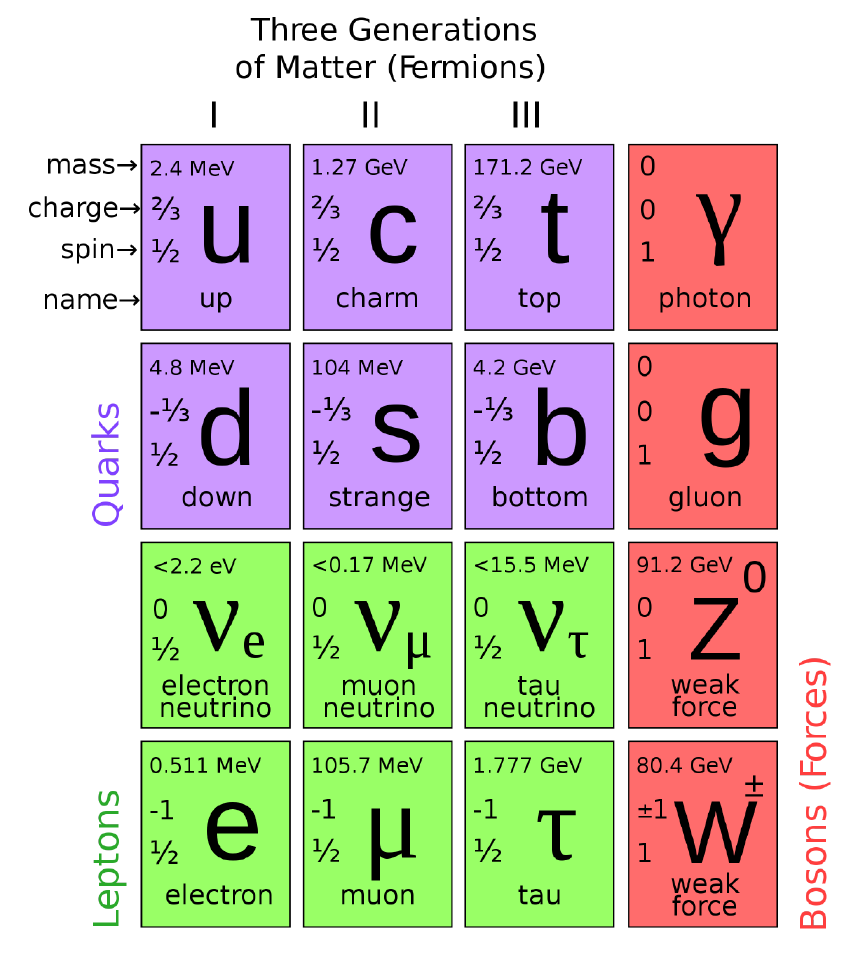
\includegraphics[width=0.65\textwidth]{theory/particles.png}


\end{tabular}
\end{center}
\caption{This figure contains fermions and gauge bosons of the SM. The Higgs boson is not included since its existents has still not been verified by experiments.}
\label{fig:particles}
\end{figure}


%\begin{table}[htb]
%\begin{center}
 %   \begin{tabular}{l|lll}
%        
%        leptons         & $\nu_{e}$ & $\nu_{\mu}$ & $\nu_{\tau}$ \\
%		        & $e$ & $\mu$ & $\tau$ \\ \hline
%        quarks   	& $u$ & $c$ & $t$ \\
%                        & $d$ & $s$ & $b$ \\
%        
%
%    \end{tabular}
%\caption{The fundamental particles of the Standard Model.}
%\end{center}
%\label{tab:particles}
%\end{table}
The three forces are introduced by gauge symmetry groups ($SU(n)$):
\begin{enumerate}
 \item $U(1)_{Y}$: Phase rotation introducing the electromagnetic forces (Sec.~\ref{sec:qed}).
 \item $SU(2)_{L}$: Weak isospin rotation explaining the weak force, combined with the $U(1)_{Y}$ to the electroweak force (Sec.~\ref{sec:electro-weak}).
 \item $SU(3)_{C}$: Rotation of the color charge leading to the strong force (Sec.~\ref{sec:qcd}).
\end{enumerate}
To keep this thesis concise while including all necessary theoretical explanations gauge invariance is only discussed in detail for QED. The weak, electro-weak unification and the strong force is only described phenomenologically.
\subsection{Quantum Electrodynamics (QED)}
\label{sec:qed}
%At the beginning of the 20th century quantum mechanics (QM) and special relativity were introduced. Attempts of combining these two theories for particles resulted in two equations for free particles. The first fundamental equation is the %Klein-Gorden-Equation describing free spin 0 particles.\\
%The second equation was formulated by Dirac and describing spin 1/2 particles. Both equations predict particles with a negative mass which lead at first to abandoning these equations. Later they were rehabilitated by interpreting these solutions as anti particles which move back in time. These particles were also discovered later.
This section demonstrates how invariance under a $U(n)$ symmetry group leads to the introduction of forces. This is being discussed for $U(1)$ with the electric charge $q$ as generator leading to electromagnetic interactions.\\ 
The basic idea of invariance is described by the Noether Theorem\cite{bib:Schmuser:FeynmanGraphs} stating that invariance under a global $U(1)$ phase transition $\Psi\rightarrow \Psi e^{-i\alpha}$ leads to the conservation of a charge $q$ and the corresponding current $J^{\mu} = q\bar{\Psi} \gamma^{\mu}\Psi$. 
The Dirac equation is invariant under such a global phase transition:
$$ \mathcal{L}_{Dirac}(\Psi \rightarrow \Psi e^{-i\alpha},\bar{\Psi} \rightarrow \bar{\Psi} e^{+i\alpha} ) =  \mathcal{L}_{Dirac}(\Psi ,\bar{\Psi} ) $$\\
This also implies that the current and thus the electric charge is conserved.\\
The interaction of particles via the electromagnetic force can be introduced by requiring invariance of the Lagrangian under local gauge transformations $U(1)$ depending on the space-time $x$:
$$ \Psi \rightarrow \Psi e^{-i\alpha(x)}.$$ 
With the usual space time derivatives $\partial_{\mu}$ this is not possible. To restore local invariance the space time derivative has to be modified by including a new gauge field $A_{\mu}$ with the following transformation:
$$ A'_{\mu} = A_{\mu}-\frac{1}{e}\partial_{\mu} \alpha(x).$$
The partial derivate is substituted by the covariant derivative $D_{\mu}$ defined as
$$ D_{\mu}= \partial_{\mu}-ieA_{\mu}   $$
resulting in the local gauge invariant Lagrangian: 
$$  \mathcal{L} =  \bar{\Psi}i\gamma^{\mu}\partial_{\mu}\Psi-m \bar{\Psi}\Psi +e \bar{\Psi}i\gamma^{\mu}\Psi A_{\mu}$$
The additional term describes the interaction of the photon $A_{\mu}$ with the fermion. An additional term $F_{\mu\nu} = \partial_{\mu}A_{\nu}-\partial_{\nu}A_{\mu}$\footnote{This is the antisymmetric field strength tensor known from classical electrodynamics.} has to be added to include the energy stored in the electromagnetic field:
$$  \mathcal{L} =  \bar{\Psi}i\gamma^{\mu}\partial_{\mu}\Psi-m \bar{\Psi}\Psi +e \bar{\Psi}i\gamma^{\mu}\Psi A_{\mu} - \frac{1}{4}F^{\mu\nu}F_{\mu\nu}.$$
This is the full QED Lagrangian including the kinetic energy of the particle and its mass together with the interaction of the particle with the Photon and the energy stored in the electromagnetic field. Similar calculations for $SU(2)_L$ and $SU(3)_{C}$ lead to weak and strong interactions. 


\subsection{The weak force and the electroweak unification}
\label{sec:electro-weak}
The weak force can be introduced by the $SU(2)_L$ group with the three Pauli matrices as generators. The $Z$ and the \W bosons are introduced as gauge bosons. In contrast to the other gauge bosons the $Z$ and \W bosons have a mass of $M_{W}=80.4$ GeV and $M_{Z}=91.2$ GeV. The resulting mass terms are not gauge invariant. Instead of direct mass terms the $Z$ and \W couple to the Higgs field (Sec.~\ref{sec:higgs}), which introduces gauge invariant indirect mass terms.\\
The weak force has been found to be maximally parity\footnote{Parity being invariance of physics under space inversion eg. $\vec x\rightarrow -x$} violating leading to exclusive left-handed\footnote{The projection of the spin vector on the momentum vector has a positive sign.} weak interactions for particles and right handed interactions for anti-particles.
The masses of the vector bosons suppresses interactions above the natural range of $10^{-18}$m, determined by the Heisenberg uncertainty principle, making the weak force appear to be weak at energies below ~100 GeV. \\
%The interaction can be written as:
%  \begin{equation}
% J^{\mu}_{weak} = \frac{1}{2}\bar{\Psi}_{1}(V^{\mu}-A^{\mu}\Psi_{2}).
%\end{equation}
%The important point is the V-A componentn in the brackets leading to maximum parity violation.
%The weak force had been introduced to explain the experimental observed $\beta$-decay. he weak force is violating parity (parity being invariance of physics under space inversion eg. $x\rightarrow -x$) making it couple only to left-handed particles. In analogy to the electromagnetic force a field quant had been introduced the $W^{+}\&W^{-}\&Z$ boson. In contrast the weak force is maximal parity violation. This leads to the structure of vector-axialvektor (V-A). The resulting weak current is being described by:
The electroweak unification describes the weak and the electromagnetic force as two aspects of the same force.
The combination can be achieved with a $SU(2)_L \times U(1)_{Y}$ group. The obtained covariant derivative $D^{\mu}$ includes 4 generators $B^{\mu}$ and $W_i^\mu$ with $i=1,2,3$.  
\begin{equation}
 D^{\mu} =  \partial^{\mu} + \frac{i}{2}g\vec \tau_i \cdot \vec W^{\mu}_i + i \frac{g^\prime}{2}YB^{\mu}
\end{equation}
with $g,g^\prime$ being coupling constants, $\tau_{i}$ defined to be the Pauli matrices.
The \W are now mixtures of the $W_{1,2}$ fields:
$$ W^{\pm} = \frac{W_1\pm i W_2}{\sqrt{2}} .$$
The $A^{\nu}$ and $Z^\nu$ are orthogonal linear combinations of the $W_3$ and $B$ fields related via the Weinberg angel $\vartheta_W = 28^\circ$ which had to measured by experiments\cite{bib:LEPEWKWG:ZPolse2005}.
$$ A^\mu =  B^\mu\text{cos}\vartheta_W +  W_{3}^\mu\text{sin}\vartheta_W $$ 
$$ Z^\mu = - B^\mu\text{sin}\vartheta_W +  W_{3}^\mu\text{cos}\vartheta_W $$
The fields $W_{1,2}$ mix to form the charged current. The electromagnetic force now couples via the hypercharge $Y$ (instead of the plain electric charge (q)):
To account for the exclusive coupling of the weak force to left handed particles $\vec T=\frac{1}{2}\vec \tau$ is defined for left handed and $\vec T = 0$ for right handed particles. The electromagnetic force still couples to both handed particles because $Y\ne 0$.\\

 
\subsection{QCD}
\label{sec:qcd}
The third force which is included in the SM is the strong force with the associated color charge and gluons as gauge bosons. The only particles carrying color charges are quarks\footnote{Anti quarks carry an anti-color.} and gluons. Experiments have shown that the color charge comes in three options introducing a new degree of freedom\footnote{For example the ratio of $e_{+}e_{-}\rightarrow \frac{hadrons}{\mu_{+}\mu_{-}}$ being three times larger than expected suggesting a new degree of freedom.}.\\ 
The gauge structure of this force is the $SU(3)_{C}$ group which is similar to the $U(1)$ group. The more complex structure of the $SU(3)_C$ leads to eight color charged gauge bosons\footnote{Either one color or anti color.} and to three and four vertex gluon-gluon interactions. The charged gauge bosons lead to the consequence that the strong force increases over distance resulting in the exclusive existence of color neutral bound states of quarks\footnote{A bound state is considered color neutral when it either consists of one color and its anti color or includes all three colors.} called hadrons. Two different kind of hadrons have been observed. Baryons, consisting of three quarks, each carrying a different color and mesons which consist of a quark and an anti-quark carrying the same color and anti-color respectively.\\
For example the proton consists of quarks and gluons called partons which have to be measured by experiments like HERA\cite{bib:CombinedHERA:2009wt}.\\
The residual of the strong force is responsible for keeping the nucleons together.



\subsection{The Higgs Mechanism}
\label{sec:higgs}
The symmetry of the $SU_{Y}(1) \times SU_{L}(2)$ has to be broken to give masses to the weak vector bosons while preserving gauge invariance. Also the photon and the gluons have to remain massless.\\
Peter Higgs\cite{PhysRevLett.13.508} among others introduced a rather simple solution to this problem. \\
His idea was to introduce a new underlaying field called Higgs field which is present everywhere in space with a degenerated\footnote{i.e. no longer invariant under symmetry transformation} lowest energy state (vacuum expectation value). The corresponding Lagrangian remains gauge invariant. The \W and $Z$ gauge boson can now couple to this field resulting in mass gathering proportional to the strength of the coupling. This symmetry breaking can be achieved while leaving the $U(1)_Y \times SU(2)_L$ symmetry unbroken therefore gauge invariant and leaving the photon massless. The $SU(3)_C$ is also not influenced.\\ 
The simplest way to produce such a so called ''spontaneous'' symmetry breaking is a complex scalar $SU(2)$ doublet with a non zero vacuum expectation value:
\begin{equation}
 \Phi(x) = \binom{\Phi_a(x)}{\Phi_b(x)}
\end{equation}
This potential can also be expressed in its four independent fields $\eta_i$ and a constant $v$:
\begin{equation}
 \Phi(x) = \frac{1}{\sqrt{2}} \binom{\eta_1(x)+i\eta_2(x)}{v+\eta_3(x)+i\eta_4(x)}
\end{equation}
With a gauge transformation $\eta_{1,2,4}$ can be absorbed by the boson fields \W and $Z$ resulting in indirect mass terms. The remaining potential
\begin{equation}
\label{eq:higgsPotential}
 \Phi(x) = \frac{1}{\sqrt{2}} \binom{0}{v+\eta_3(x)}
\end{equation}
is now independent of $\eta_{1,2,4}$.
The corresponding gauge invariant Lagrangian is:
\begin{equation}
 \mathcal{L}_\Phi(x) = (D^\mu\phi(x))(D_\mu\phi(x))-\mu^2|\phi(x)|^2-\lambda|\phi(x)|^4-\frac{1}{4}F^{\mu\nu}(x)F_{\mu\nu}(x)
\end{equation}
with $\phi(x)$ being the scalar Higgs field, $F^{\mu\nu}(x)$ the Lagrangian density of the free field, $D^\mu$ the covariant derivative, $\mu^2$ and $\lambda$ being real parameters. No mass-term for the $\gamma$ is being introduced therefore the $\gamma$ remains massless. A minimum of the potential exists at
$$\nu = \sqrt{\frac{-\mu^2}{\lambda}} $$ 
when $-\mu^2 > 0$ and if $\lambda$ is a real parameter. This minimum can be identified with the vacuum expectation value of the Higgs field, also included in Eq.~\ref{eq:higgsPotential}. A massive spin 0 Higgs boson with the mass of $M_H = \sqrt{-2\mu^2}$ is the consequence of the remaining free Higgs field $\eta_3(x)$.\\
In addition to the mass generation of the weak vector bosons the Higgs mechanism provides also an elegant way for fermions to acquire masses\footnote{In principle neutrinos could also gather masses in the same way but the SM assumes them to be massless.}.
%The potential is rotation symmetric around the origin and has a minimum $v$ at $ v = \frac{\mu}{\lambda}$ as can be seen in fig.\ref{fig:higgs}. Since at $v=0$ no minimum exists and nature always realizes the condition of lowest energy the by construction rotation symmetry is broken and the vacuum expectation value of the Higgs Field is $\frac{v}{\sqrt{2}}\ne 0$.\\ 
%Terms introduced when making the Lagrangian gauge invariance lead to self coupling of the Higgs potential resulting in a massive vector boson the Higgs boson with a bare mass of $ M_{H}=\sqrt{-2\mu^{2}} $. Since $\mu$ is a free parameter the mass of the Higgs boson can not be calculated however precision measurements at LEP exclude a Higgs Boson with masses less than $114$~GeV and masses of more than $600$~GeV are also disfavored. CMS, Atlas and the Tevatron have discovered coherent excesses around $124$~GeV, but the statistical significance is not yet enough for a discovery.\\ 
%The Lagrangian of charged (electric and/or color) fermions can also not contain mass terms while being gauge invariant. However the Higgs mechanism provides also the possibility for fermions to gather masses. The mass term $m_{a}=\lambda_{a}\frac{v}{\sqrt{2}}$ with $a$ being any charged lepton or quark describes the coupling of the fermions to the Higgs field and leads to mass gathering. The coupling constant is a free parameter making the Higgs mechanism able to give to all particles masses but does not explain why the masses are from such different magnitudes.\\
%Neutrinos could in principle gather with the same mechanism masses but are not included in the standard definition.



\section{Open questions and problems of the SM}
\label{sec:SM_problems}
Despite all achievements of the SM in not only describing but predicting particles and interactions it can only be seen as a low energy approximation of a more fundamental theory. The following list provides some short comings of the SM and experimental results hinting towards new physics for which a popular approach will be discussed in the following chapter. 

\begin{itemize}
 \item The weak and electromagnetic force have been unified suggesting the idea of unifying every force within a theory of everything. Such Grand Unified Theories (GUTs), unify the electro-weak and the strong force at an energy around $10^{15}$~GeV in a gauge group $G$ with one single coupling. The SM can not provide such a unification at such a scale. 

 \item All the particles masses can not be predicted within the SM but have to be measured. Further the exact same value of the electric charge for the electron and the proton can not be explained. Also at very high energies radiative corrections to certain processes diverge leading to unitarity violation.

 \item Astrophysical observations have shown discrepancies between expected mass distributions calculated from galaxy gravitational lensing and the visible amount of matter, suggesting a huge amount of dark matter, about 23\% of all energy within the universe \cite{Bertone2005279}. Dark matter does not interact electromagnetically or strongly making it invisible to direct observations. The neutrinos are the only candidates within the SM for such matter but observations require dark matter to be a lot heavier than the upper limit on the neutrino masses. 

 \item Another problem within the SM is the so called ''Naturalness''. The bare Higgs mass $M_{H}$ introduced in Sec.~\ref{sec:higgs} has to be corrected by higher order quadratic loop corrections. If the SM is valid up to the Plank scale ($10^{19}$~GeV), at which gravity becomes as strong as the other forces, loop corrections would increase the Higgs mass significantly. To reduce the mass of the Higgs boson to the favored O(100 GeV) regime, so called ''fine tuning'' is needed. Different independent loop corrections with opposite sign would have to cancel each other to a precision of $10^{-31}$ which is not convincing.

 \item A different approach to solve the Naturalness problem is the introduction of a cut-off energy scale at which new physics is expected. A cut-off at the TeV scale solves the Naturalness problem by demanding new particles with such a mass. Supersymmetry as discussed in Sec.~\ref{sec:susy} can provides such particles and therefore is believed to be realized at the TeV scale making it potentially discoverable by LHC experiments.

 \item Furthermore every attempt to combine gravity and the SM has failed so far.

 \item Also the observed asymmetry of matter and anti-matter can not be explained.

\end{itemize}
%In order to bring the mass of the Higgs Boson to the GeV scale which is in favor of many experimental and theoretical results finine tuning is need which would mean a precision of $10^{34}$ in the Lagrangian mass parameter.\\
These reasons among others lead to the assumption that the SM can only be seen as a low energy approximation of a more fundamental theory.\\




%Several cosomological observations suggest the existing of an additional form of matter called dark matter. Dark matter interacts only weakly and via gravity making it invisible to electromagnetic observations. From measurments of rotation curves the dominating force gravity does not explain how stars are moving unless additional matter is present. Neutrinos interact only weakly and if they are not massless via grvaity but from calculations of the early univers dark matter has to be ``cold'', meaning that the particles have to be non relativistic and a lot heavier than the upper limits on the neutrino masses.\\

%Another problem within the SM is the so called  ``Naturalness of the SM''. The plain Higgs mass $M_{H}$ introduced in sec.\ref{sec:higgs} has to be corrected by higher order loop corrections. If the SM is valid to very high energies up to the Plank scale ($10^{19}$~GeV) at which gravity becomes compatibly strong to the other forces loop corrections would increase the Higgs mass significantly. To reduce the mass of the higgs boson to the favoured GeV regime so called ``fine tuning`` is needed. Different independent loop corrections with opposite sign would have to cancel each other to a precision of $10^{-31}$ which is not convincing.\\

%One of the most obvious short comes of the SM is the lack of integrating gravity. Also the observed asymmetry of matter and anti-matter can not be explained.

\section{Supersymmetry}
\label{sec:susy}
Many theories are available which solve some of theses short comings. A very elegant approach of solving the fine tuning problem and providing a dark matter candidate is Supersymmetry (SUSY). Since this thesis focuses on the search for new physics and especially for SUSY particles an introduction to SUSY will be presented in the next section.
Supersymmetry (SUSY) is the last possible symmetry operation which can be incorporated into the Poincar$\acute e$ group\cite{bib:Aitchison:Susy}. The SUSY generator $Q$ relates fermions and bosons and in its simplest version introduces for each SM particle a supersymmetric partner with a shift in spin of 1/2. Therefore, the SUSY partners of the fermions are bosons with spin 0 called sfermions and the partners of the SM gauge bosons are spin 1/2 fermions called gauginos. In addition another Higgs doublet has to be introduced resulting in five Higgs bosons instead of the one predicted by the SM. The color neutral gauginos and the higgsinos mix to form four charged charginos $\chi^{\pm}_{1,2}$ and four neutral neutralinos $\chi^{0}_{1-4}$.\\
The generator $Q$ commutes with all SM generators resulting in identical quantum numbers and masses of the related particles.\\
Besides the argument that it can in principle be added to the Poincar$\acute e$ group SUSY can also solves many problems of the SM for example the ''Naturalness'' problem. The quadratic loop corrections from SM particles are countered by the SUSY particles that enter with opposite sign.\\
SUSY allows terms which violate baryon- and lepton-number conservation. One consequence is that the proton becomes unstable. The decay is mediated by the product of one lepton- and one baryon-number violating term. The lower limit on the life time of the proton has been found to be $6.6 \cdot 10^{33}$ years \cite{Ahmed:2003sy}\cite{PhysRevLett.102.141801} putting tight boundaries on the decay and therefore on the corresponding terms in the Lagrangian.\\
To recover the proton stability a new conserved quantity, $R$-party, is introduced:
$$ R = (-1)^{3(B-L)+2S}$$
with $B$ being the baryon-number, $L$ the lepton-number and $S$ the spin. SM particles have $R=1$ and SUSY particles have $R=-1$ prohibiting the mixing between SM and SUSY particles.\\
An interesting consequence of R-parity conservation is the stability of the lightest supersymmetric particle (LSP) making it a natural candidate for Dark Matter if it interacts only weakly.\\
So far extensive searches have been conducted for SUSY but none has found any direct evidence for its existents yet (eg.\cite{D0Limits}\cite{CDFLimits}\cite{L3SUSY}). The SUSY particles have to have the same mass as the SM partners but no such particles have been found. This problem can be solved when SUSY is a broken symmetry. For soft broken SUSY more than 100 new free parameters have to be introduced in the most general case.\\
The breaking mechanism is believed to take place at the GUT scale in a so called ''hidden sector'' which is decoupled from the observable universe below the breaking scale. The mass term breaking is mediated via messenger interaction mediated to the observable universe. All soft breaking mechanisms involve gravity as messenger interaction. For mSUGRA gravity is assumed to be the only one.
%Among others gauge-meditated breaking where additional gauge interactions are assumed to communicate the effects of SUSY breaking from the hidden to the observable sector and gravity-mediated breaking where gravitational interactions transmit the breaking have been developed.



\subsection{SUSY breaking in the Model of Minimal Supergravity and the cMSSM}
\label{sec:msugra}
Minimal Supergravity Models (mSUGRA) are favored for presenting experimental results since they include only five free parameters which makes result interpretation easier.\\
In mSUGRA the mass breaking from the hidden sector is transmitted via gravity\footnote{ The graviton couples to the energy-momentum tensor for matter from general relativity. Still the Supergravity Lagrangian has some non-renormalizable parts. Therefore this can not be seen as a proper implementation of gravity but at best as a low-energy approximation.}.
The large amount of over 100 free parameters is reduced to only five by implying that the strength of all gauge coupling parameters become equally strong and unification of the common scalar and gaugino mass breaking terms at the GUT scale\footnote{$\Lambda \approx 10^{16}$ GeV}. The remaining free parameters are:
\begin{equation}
 m_0,m_{1/2},A_0,\text{tan}\beta,\text{sign}(\mu)
\end{equation}
With $m_0$ being the common mass breaking parameter for all sleptons, squarks at the GUT scale, $m_{1/2}$ being the mass of the gauginos at the GUT scale, $A_0$ is the trilinear scalar coupling between the Higgs and two sfermions, $\mu$ being the Higgs mass parameter and $\text{tan}\beta = \frac{v_u}{v_d}$ is the ratio of the two vacuum expectation values arising from the two Higgs fields.\\
From renormalization group equations the couplings and masses at low energy scales can be obtained.\\
In mSUGRA models the ratio $\text{tan}\beta$ is fixed were in cMSSM it can be varied. The results of this analyses are presented within the cMSSM framework and Simplified Models (Sec.~\ref{sec:cMSSM}, ~\ref{sec:simplified}).





%SUSY introduces a new symmetry operation with the generator $Q$ which invokes a spin shift of $\frac{1}{2}$.
%\begin{equation}
% Q|\text{fermion}> = |\text{boson}> ; Q|\text{boson}> = |\text{fermion}>
%\end{equation}
%The generator $Q$ commutes with all generators of the SM resulting in the exact same quantum numbers and mass for two related particles. Since no evidence of supersymmetric particles with the same masses as the SM partners has been found experimentaly, SUSY must be a broken symmetry if realized in nature.\\\\
%In principle SUSY allows terms which violated baryon- and lepton-number conservation. Lower limits on the life time of the proton of $2.1 \cdot 10^{29}$ years\cite{Ahmed:2003sy} , have put tight boundaries on the strength of such terms.
%A new quantum number $R$-parity is introduced which when conserved sets these violating terms to 0 making the proton stable.  $R$-parity defined as:
%$$ R = (-1)^{3(B-L)+2S}$$
%with $B$ being the baryon-number, $L$ the lepton-number and $S$ the spin. SM particles have $R=1$ and SUSY particles have $R=-1$ leading to the prohibition of mixing between SM and SUSY particles.\\

%Some of the short comes of the SM can be solved or at least reduced by indroducing SUSY:
%\begin{itemize}
% \item If R-parity is conserved the lightest supersymmetric particle (LSP) must be stable. This particle is a natural candidate for the expected Dark Matter in the universe.
% \item The Naturalness problem is reduced significantly by the additional loop corrections from SUSY particles on the Higgs mass.
% \item The observed asymmetry between baryons and anti-baryons can be explained by SUSY interactions.
% \item The gauge couplings are modified leading to a unification of forces at the GUT scale as illustrated in fig.\ref{fig:runningCoupling}.
% \item The divergencies arising when applying quantum field theory on gravity are reduced. Still gravity can not be included but it appears to be a good step in the direction of unification.   
%\end{itemize}
%In gernal SUSY introduced a huge amount of new free parameters resulting in a immens amount of possible SUSY models. In the following two modells with R-party conservation and strong other constraints are discussed and the results of the analyses will be discussed in this context.

%\subsection{MSSM and cMSSM}
%\label{sec:susy_cMSSM}
%Both the cMSSM and the Simplified Models are based on the Minimal Supersymmetric Model (MSSM). Minimal stands for the least possible amount of additional particles to the ones included in the SM. In addition to the superpartners of the particles another Higgs doublet field has to be introduced resulting in five Higgs bosons instead of one. Also $R$-Parity conservation is implemented.\\
%The Lagrangian for the MSSM  consists of three terms: 
%\begin{equation}
% L_{MSSM} =  L_{gauge} + L_{F} + L_{soft}
%\end{equation}
%The gauge part is complete determined by requiring gauge-invariance and super-symmetry. $L_F$ describes the couplings derived from the superpotential.\\
%The lack of any experimental direct evidence of SUSY particles leading to the higher assumed masses must be introduced by hand into the superpotential. $L_{soft}$ includes all possible soft SUSY breaking operators. To keep the advantage of solving the Naturalness problem and avoid renormalization problems this mechanism is very constrained leading to the chosen name ''soft'' of the breaking terms.\\
%How this breaking mechanism is realized in nature is beyond the understand of todays knowledge. It is believed that the breaking takes place in a sector which is separated from the observable universe, the so called ''hidden'' sector. Different ideas have been presented explaining how the interaction is mediated from the hidden sector. Among others the so called mSUGRA (minimal super gravity) is able to explain the different masses by mediating the interaction of the hidden sector and the (s)particles via gravity.\\
%The MSSM introduces 178 free parameters which makes it very difficult to do phenomenological analysis.\\
%The cMSSM is a constrained version of the MSSM. These constrains arise from assuming gauge coupling unification and the constrains from electro weak symmetry breaking. Only five independent free parameters are left within the cMSSM.
%\begin{equation}
% m_{0}, m_{1/2}, A_{0}, tan\beta, \text{and} sign(\mu)
%\end{equation}
%With $m_0$ being the common mass for all sleptons, squarks  and Higgs bosons at the GUT scale, $m_{1/2}$ being the mass of all gauginos at the GUT scale, $A_0$ is the trilinear scalar coupling between the Higgs and two sfermions and $\mu$ being the Higgsino mass parameter. 
%Where $m_0 / m_{1/2}$ are the unified masses at the GUT scale. $tan\beta = \frac{v_u}{v_d}$ is the ratio of the two vacuum expectation values arising from the two Higgs fields.


%\subsection{Simplified Models}
%\label{sec:susy_simplifiedModels}






%susy.
%allgemein was ist susy welche annahmen:




%welche konsequenzen ergeben sich daraus:
% Loest das hirachie problems
% proton instabil


%experimentelle datan:
% proton stabilisieren durch r partiy
% -> guter kandidat fuer dark matter
 

% susy nicht gefunden
% -> massenbrechung

%  kurz auf das prinzip der massenbrechung eingehen


%specielles modells
%
%   MSUGRA
%  -> cMSSM  unterschied beta anders



%simplified models

%topologie festlegen:

%allgemeiner neue teilchen werde produziert mit massen und zerfalls verhaeltniss
% wirkungsquerschnitt wird als benchmark auf qcd wirkungsquerschnitt gesetzt mal 3 durch 3 um abhaengigkeit von wirkungsquerschnitt zu zeigen

%oset<->simplified models










 

\cleardoublepage

\chapter{LHC and CMS detector}
\label{sec:detector}
\section{The Large Hadron Collider (LHC)}
\label{sec:LHC}
The Large Hadron Collider (LHC)\cite{1748-0221-3-08-S08001}\cite{Bruning:782076}\cite{ipac11:lamont} is the largest and most complex machine every build by man. It is a circular proton-proton collider in a tunnel 100 meters below surface at the CERN research center close to Geneva, inheriting the former Large Electron Positron collider (LEP) tunnel with a circumference of 26.7 km. Fig.~\ref{fig:LHC} shows the layout of the LHC and the vaults containing the experiments. \\
\begin{figure}[tbhn]
\begin{center}
%\begin{tabular}{cc}
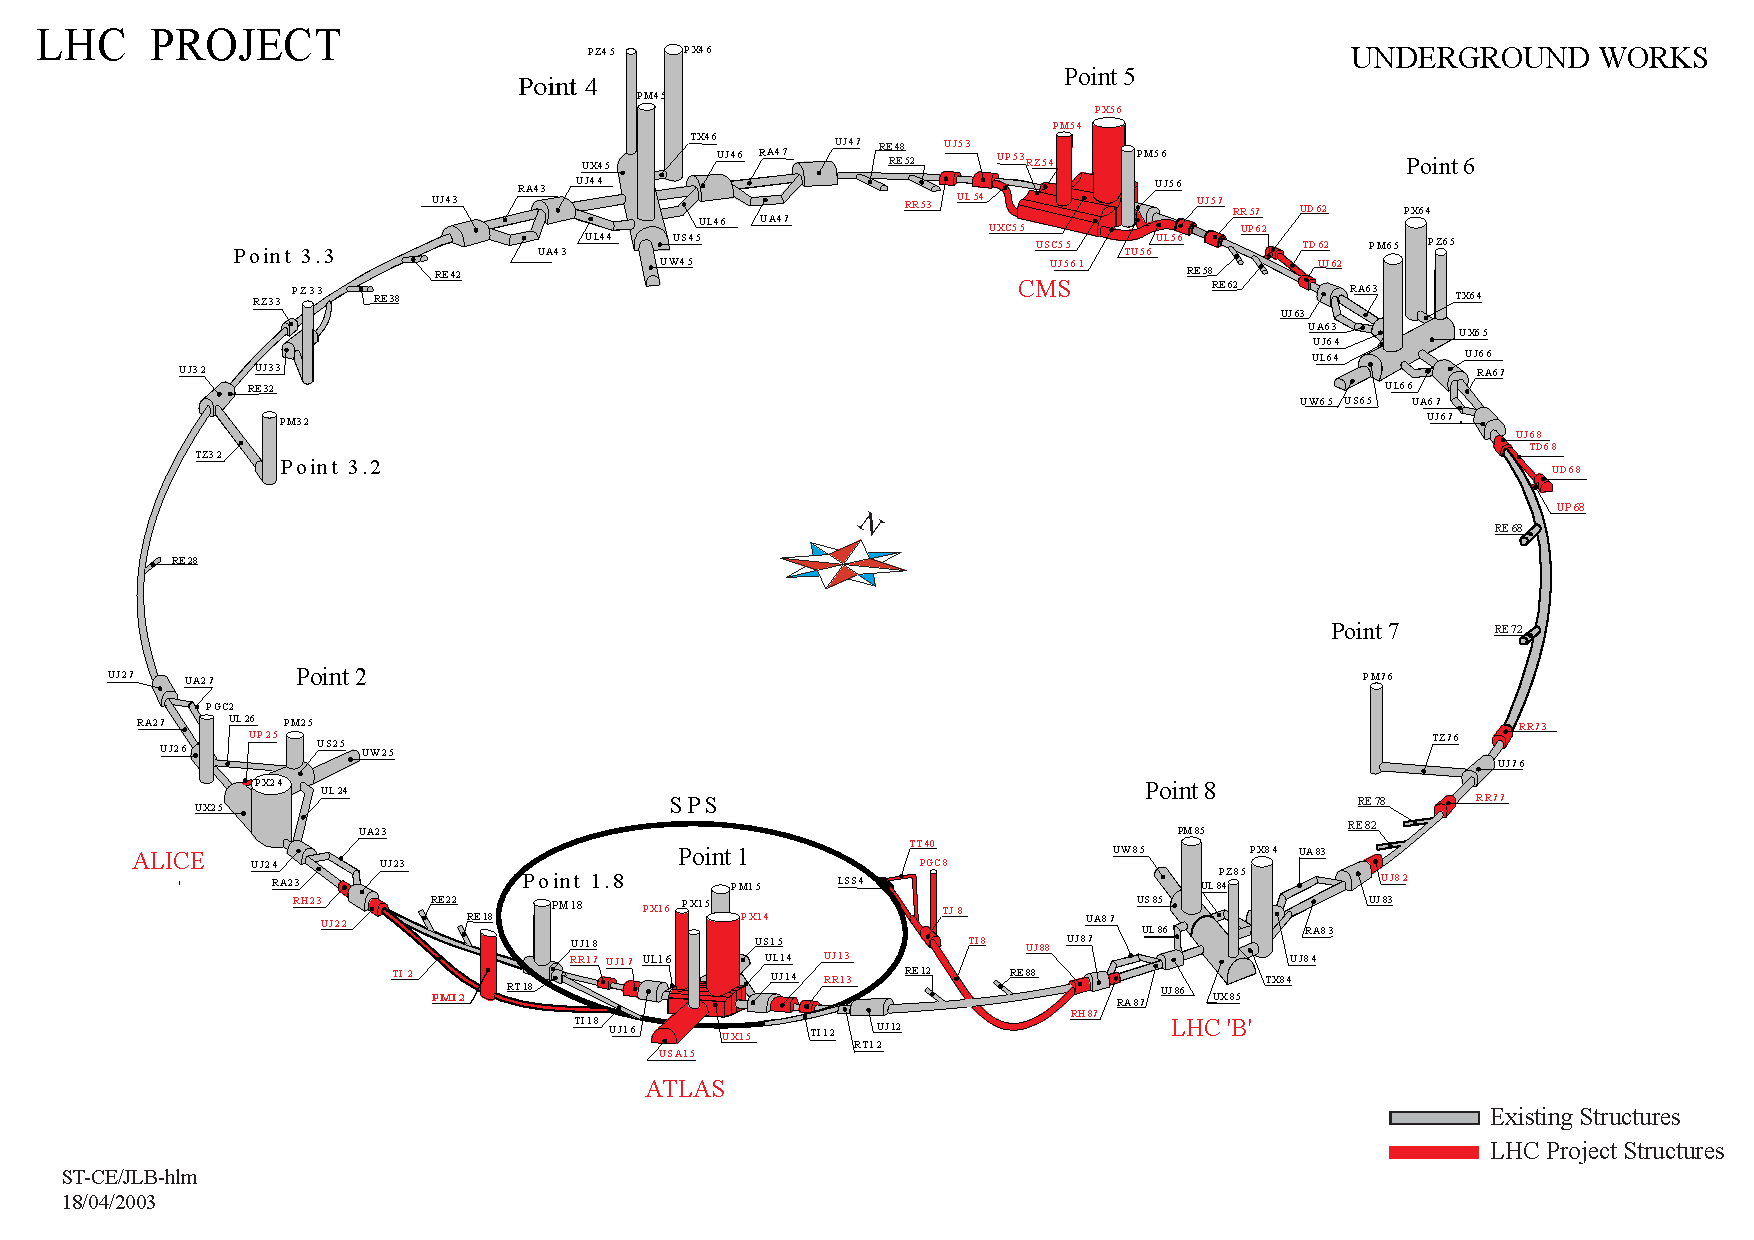
\includegraphics[width=0.85\textwidth]{detector/figures/LHCUnder.pdf}
%\end{tabular}
\end{center}
\caption{An exploded view of the CMS detector.}
%%The bin-by-bin combination of the background contributions and their uncertainties has been performed in a simplified way assuming Gaussian probability distributions.}
\label{fig:LHC}
\end{figure}




The LHC was designed for a center-of-mass energy of 14 TeV and a luminosity of $L = 10^{34} cm^{-2}s^{-1}$. The luminosity $L$ is defined as:
\begin{equation}
 L = \frac{N^{2}_{b}n_{b}f_{rev}\gamma}{4\pi \epsilon_{n}\beta^*}F
\end{equation}
where $N_{b}$ is the number of particles per bunch, $n_b$ the number of bunches per beam, $f_{rev}$ the  revolution frequency, $\gamma$ is the Lorentz factor, $F$ a reduction factor arising from the angel of the two beams at the interaction, $\epsilon_n$ a quantity of the parallelism of the beam and $\beta^*$ is related to the width of the beam at the interaction point.\\
The design Luminosity can be achieved with 2808 bunches colliding every 25 ns, an $\epsilon_n=3.75$ $\mu\text{m}$ and a $\beta^* = 0.55$ m.\\ 
Strong magnetic fields of up to 8,4 Tesla are needed to keep the high energetic protons with a maximum energy of 7 TeV circling. To achieve such high magnetic fields superconducting magnets have been chosen.\\
The particles are collided at specific interaction points at the four main detectors ATLAS\cite{det::ATLAS}, CMS\cite{bib:cmsptdr1}, LHCb\cite{det::LHCb} and ALICE\cite{det::ALICE}.
ATLAS and CMS are multipurpose detector designed with the focus on the discovery of the Higgs boson, search for physics beyond the SM and top physics, while LHCb focuses on the CP-violation in b-physics and ALICEs was designed to investigate quark-gluon plasma produced in heavy ion collisions.\\
This thesis analysis makes use of a total luminosity of \lumi\cite{CMS-PAS-EWK-11-001__} of proton-proton collisions with at a center-of-mass energy of 7 TeV and a peak luminosity of $L = 3.55 \cdot 10^{33} cm^{-2}s^{-1}$ recorded by the CMS detector during the year 2011.\\
The following chapter contains a description of the CMS detector and its components followed by an introduction to the physics objects and definitions relevant for this analyses and the particle flow algorithm used for particle reconstruction.
\clearpage









\section{The Compact Muon Solenoid detector}
One main aspect relevant for the design of the Compact Muon Solenoid (CMS) was the inclusion of the calorimeters within a strong magnetic field to measure charged particles and especially muon momenta to a high precision. To achieve high the magnetic field, a superconducting magnet was installed.\\
The CMS detector is built in cylindrical shape around the beam pipe with a length of 21.6 m and a diameter of 14.6 m with a total weight of of 12 500 tons. Fig.~\ref{fig:CMS} shows an overview of the CMS detector.\\
\begin{figure}[tbhn]
\begin{center}
%\begin{tabular}{cc}
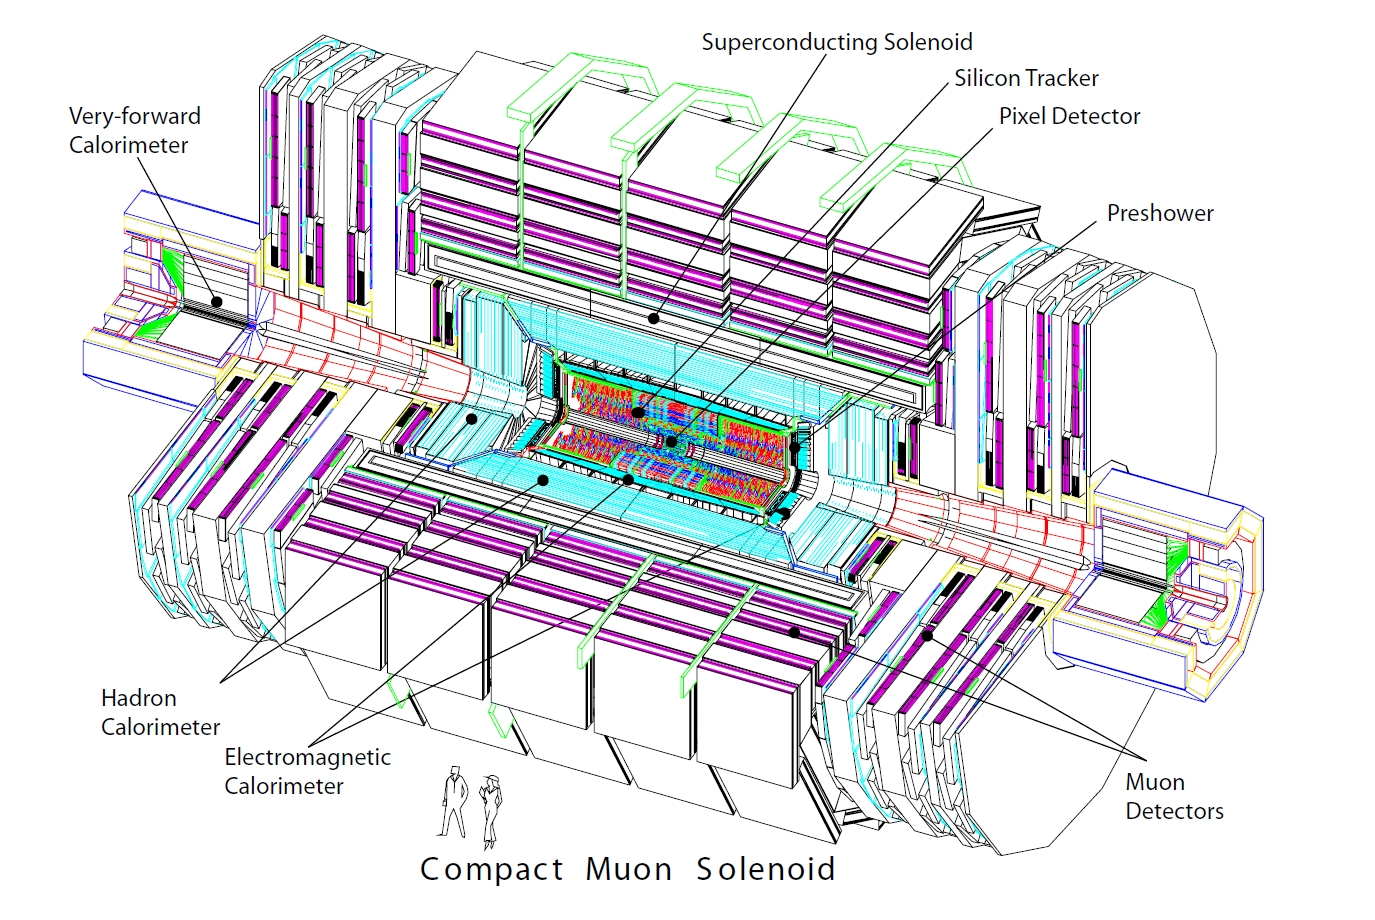
\includegraphics[width=0.85\textwidth]{detector/figures/CMS.jpg}
%\end{tabular}
\end{center}
\caption{An exploded view of the CMS detector.}
%%The bin-by-bin combination of the background contributions and their uncertainties has been performed in a simplified way assuming Gaussian probability distributions.}
\label{fig:CMS}
\end{figure}
\clearpage
A right-handed coordinate system together with cylinder coordinates has been chosen by the CMS collaboration.
With the z-axis pointing in the beam direction, y-axis pointing up and the x-axis pointing to the center of the LHC. The polar angel $\Theta$ is measured from the z-axis and the azimuthal angel $\phi$ is measured relative to the x-axis in the x-y plane.
The pseudorapidity $\eta$, commonly used in high energy physics, is given by:
$$ \eta = - \text{ln tan}\left(\frac{\Theta}{2}\right)  $$
The Lorentz-invariant distance between two relativistic objects is defined as:
$$ \Delta R= \sqrt{(\Delta\eta)^2+(\Delta\Theta)^2} $$
Since the initial momentum in the beam direction (z) for interactions at hadron colliders like the LHC is unknown, only the transverse\footnote{relative to the beam axis} momentum $p_T =p \cdot \text{sin}\Theta$ and the transverse energy $E_T = E \cdot \text{sin}\Theta$ is used to measure the energy and momentum of produced particles.\\
The following layers are cylindrically build around the beam pipe:
\begin{itemize}
 \item A silicon-based tracker (Sec.~\ref{sec:tracker}) at the heart of the detector designed to measure the trajectory of particles with a high precision.
 \item The next layer consists of the electromagnetic calorimeter (ECAL)(Sec.~\ref{sec:ecal}) based on scintillating crystals mainly used to detect electrons and photons.
 \item A preshower system has been installed in front of the ECAL endcaps, designed to identify $\pi^0$ particles.
 \item The Hadronic calorimeter (HCAL)(Sec.~\ref{sec:hcal}) surrounding the electromagnetic calorimeter is designed to measure jet energies.
 \item To improve the HCAL ability to measure high energetic jets a ''tail-catcher'' in the barrel region has also been installed.
 \item The outermost part of the detector consists of the iron yokes for the magnetic field together with the drift chambers together forming the muon detection system (Sec.~\ref{sec:muonchambers}).
\end{itemize}
These sub parts of the CMS detector will be discussed in greater detail in the following.
\clearpage


\subsection{The tracker}
\label{sec:tracker}
Fig. ~\ref{fig:tracker} shows the layout of the CMS tracker\cite{Chatrchyan:2008zzk}\cite{bib:cmsptdr1}\cite{bib:cmstdr:tracker} which extents to 1.1 m in transverse direction and is approximately 5.4 m long.\\
\begin{figure}[tbhn]
\begin{center}
%\begin{tabular}{cc}
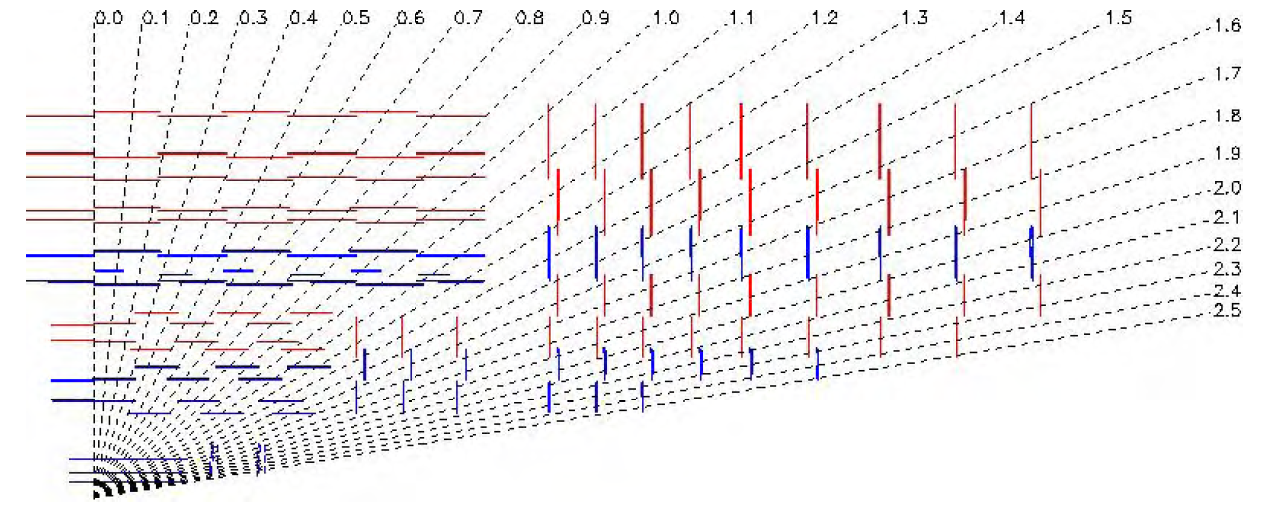
\includegraphics[width=0.85\textwidth]{detector/figures/tracker.png}
%\end{tabular}
\end{center}
\caption{An exploded view of the CMS detector.}
%%The bin-by-bin combination of the background contributions and their uncertainties has been performed in a simplified way assuming Gaussian probability distributions.}
\label{fig:tracker}
\end{figure}
The inner tracker is divided in two parts:\\
The pixel detector consists of 55 million pixels because close to the interaction point a high granularity is necessary due of the high particle flux. Also a high resolution of the vertex reconstruction of 25 $\mu$m and 20 $\mu$ m in X and Y is needed\cite{CMS-PAS-TRK-10-005}. This high resolution is especially important in measurements of b-jets since they have a relative long lifetime resulting in a measurable transverse distance of a second vertex of the decaying b-jet. The high design instantaneous luminosity leads to additional interactions in one bunch-crossing called pileup interactions. These usually soft interactions need to be separated from the hard process which requires good resolution.\\
The second part is the silicon strip detector located outside of the pixel detector. A total area of 200 $\text{m}^2$ is covered by 9.6 million strips covering, the region up to $|\eta| \approx 2.4$.\\
The reconstruction efficiency of muons with a $\pt > 1$ GeV is about 99\%.
Combined with the strong magnetic field tracks of charged particles can be measured to reconstruct the transverse momentum according to this equation:
$$ \pt = 0.3\frac{\text{GeV}}{e \cdot \text{T} \cdot m} \cdot B \cdot \rho$$
with B being the magnetic flux density, $\rho$ the tracks radius of curvature in the transverse plane, $m$ and $e$ being the mass and the electric-charge of the particle.


\subsection{The Electromagnetic Calorimeter}
\label{sec:ecal}
The homogeneous electromagnetic calorimeter (ECAL)\cite{Chatrchyan:2008zzk}\cite{bib:cmsptdr1}\cite{bib:cmstdr:ecal} was build around the inner tracker system consisting of lead-tungstate crystals, which have a radiation length\footnote{The length after which an electrons energy has decreased to $\frac{1}{e}$ of its original energy.} $X_0 = 0.98$ cm and a Moliere radius of $R_M = 2.2$ cm resulting in a compact size which is especially important to fit the tracker, ECAL and the HCAL inside of the Superconducting Solenoid.\\
The barrel part of the ECAL consists of 61 200 crystals covering $|\eta| < 1.479$ whereas the two endcaps are build up of 14 648 crystals covering $ 1.479< |\eta| <3.0$.\\
The crystals are robust against radiation and emit 80\% of the light radiated within the 25 ns between two bunch crossings at design LHC operation. The ECAL has an energy resolution of 
$$ \left(\frac{\sigma}{E} \right)^2= \left(\frac{\text{S}}{\sqrt{E}} \right)^2 +\left(\frac{\text{N}}{E}\right)^2+ \text{C}^2 $$
with S=3\% as stochastic term, N = 124 MeV as noise term and C = 0.26\% as constant term.	
The response of a calorimeter is defined to be the measured energy divided by the true energy of a particle showering. Hadrons and electrons have a different response with the ratio given by $\frac{e}{h}\approx 1.6$. Noise is being suppressed by only reading out cells with an energy deposited above a certain threshold.\\
Good performance of the ECAL has been observed however some of the about 70 000 crystals have a dysfunctional readout.


\subsection{The Hadronic Calorimeter}
\label{sec:hcal}
The Hadronic Calorimeter (HCAL)\cite{Chatrchyan:2008zzk}\cite{bib:cmsptdr1}\cite{bib:cmstdr:hcal} consists of alternating layers of brass as absorber and plastic scintillators. To support these heavy structures the innermost and outermost layers are made of steel. The ECAL and HCAL are arranged in towers read out by single wavelength shifting fibers.\\
The HCAL consists of four parts:
\begin{itemize}
 \item The hadron barrel (HB) covering the central part of the HCAL with $|\eta| < 1.4$ made of 2304 towers with a segmentation of $\Delta \eta$ x $\Delta \Phi = 0.087$ x $0.087$. The absorbers have the thickness of 5.05 cm for each of the inner eight layers and 5.56 for the outer six layers. The scintillators located in between the absorber layers are 3.7 mm thick except for the very first layer behind the ECAL which is 9 mm thick. 
 \item Due to the limited space available by keeping the HCAL inside the Solenoid, jets may not deposit their entire energy within this part. Scintillators are also outside the coil with an interaction length of 1.4/sin($\Theta$) called the hadron outer detector (HO)\footnote{This part was not used for the analyzed data in this thesis since the noise level was not sufficiently small.}.
 \item The hadron endcaps (HE) make up the third part. Here only 87 mm thick brass and one 3.7 mm thick scintillator was used. 
 \item The last part the hadron forward (HF) is located close to the beam axis at   $3.0 <|\eta| < 5.0$. This part is made of steel absorber and radiation hard quartz fibers. It is constructed out of 18 wedges located 11 m from the interaction point thus increasing the coverage helping to measure missing transverse momentum.
\end{itemize}
Like the ECAL the HCAL is a non-compensating calorimeter with $\frac{\text{e}}{\text{h}}\approx 1.4$. A read out threshold is also used to reduce noise (called zero suppression).



\clearpage
\subsection{The Solenoid and the Muon Chambers}
\label{sec:muonchambers}
The superconducting solenoid with a length of 12.9 m, a thickness of 1.8 m and an inner diameter of 5.9 m is one of key element of the CMS detector dominating its design. 19.5 kA of current are used to provide the 3.8 Tesla magnetic field which permeates the calorimeter and tracker.\\
The muon chambers\cite{Chatrchyan:2008zzk}\cite{bib:cmsptdr1}\cite{bib:cmstdr:muon} localed outside the magnetic coil partially taking advantage of the material used for the solenoid consist of four muon stations covering $|\eta|<2.4$.
The muon barrel region (MB) uses aluminum drift tube chambers (DT) to achieve high resolution for muons. The endcaps (ME) consist of cathode strip chambers (CSCs). In this forward direction a higher rate of muons is expected explaining the use of CSCs due to their fast response. The coverage is being completed by resistive plate chambers (RPCs) included in both parts of the muon chambers. These RPCs have a much lower momentum resolution than the other parts of the muon chambers but the very fast response time and the excellent time resolution is needed to identify the correct bunch crossing. These muon detectors are arranged in four stations in both detector regions.\\
Together with the inner tracker the muon system is able to achieve a muon \pt resolution between 1\% and 10\% up to a muon \pt of 1 TeV.




\subsection{Trigger}
\label{sec:trigger}
At design luminosity the LHC has a bunch crossing rate of 40 MHz. At this rate the event size of approximately  1 MB per event leads to a too high output of data to be stored and processed. Since not all events include interesting physics a trigger system\cite{bib:cmstdr:trigger}\cite{bib:trigger:summerschoollecture} only collecting events fulfilling predefined criteria is installed.\\
The trigger is organized in two stages:
\begin{itemize}
 \item The pure hardware\footnote{Pure hardware trigger was chosen since it has increased speed compared to software triggers.} level 1 trigger(L1) using only detector parts which have a fast readout rate, the calorimeters and the muon chambers. These informations are combined by simplified object algorithms to loosely define electrons, photons, muons and jets. From these algorithms interesting events are selected by demanding a certain energy threshold and or leptons or jets to reduce the event rate to 100 kHz\footnote{Prescaled trigger paths are used to collect only every x-th collision of one type of interaction, important for collisions which have a too high rate to recored every collision.}. To keep the information until the L1 has decided weather an event will rejected or not the full detector output is stored in a pipeline for 3.2 $\mu$s.
 \item The software based high level trigger (HLT) which is also used to reduce the amount of events further by a factor of 100 to be able to store the events at a rate of $\approx 100$ MB/s. This trigger can access the full detector information enabling more advanced trigger algorithm definitions. The advantage of software based triggers compared to hardware based ones is the flexibility in the design of individual trigger paths. Restrictions from the aim of a reduction factor of 100 together with the demands from physical analysis dominate the trigger paths designs. 
\end{itemize}
Each stored event inherits the L1 and HLT trigger informations.
 

\section{Particle identification and physical object definitions}
\label{sec:physics_objects}
This section covers particle identification of the CMS detector and physics quantities used in this thesis.\\
The particles emerging from the interaction point at the center interact differently with the detector components enabling distinguishing between them. Fig.~\ref{fig:particlePassing} illustrates typical interactions with the detector components.
\begin{figure}[tbhn]
\begin{center}
%\begin{tabular}{cc}
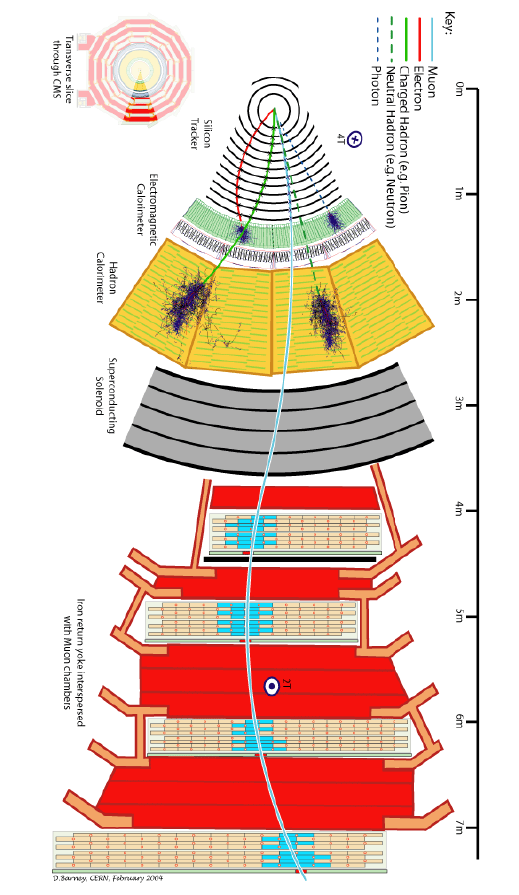
\includegraphics[width=0.75\textwidth]{detector/figures/particlePassing.png}
%\end{tabular}
\end{center}
\caption{This figure shows the transverse slice through the CMS detector with typical particle interaction signatures with the detector.}
%%The bin-by-bin combination of the background contributions and their uncertainties has been performed in a simplified way assuming Gaussian probability distributions.}
\label{fig:particlePassing}
\end{figure}

This list covers typical signatures of photons, electrons, muons, taus, jets and only weakly interacting particles:

\begin{itemize}
 \item Photons are electrical neutral particles thus leaving in most cases no track in the tracker. First interactions happens typically in the ECAL. Due to the depth of $X_0=25$ of the ECAL photons are most likely to deposit all energy distributed only over a few crystals in the ECAL. Approximately 50\% of all photons already convert to $e^-e^+$ pairs within the tracker but usually the major fraction of energy is deposited in the ECAL\cite{CMS-PAS-EGM-10-005}.
 \item Electron identification is difficult because of the emission of Bremsstrahlung. Due to the high magnetic field and the strong resulting bending of the electron trajectory the emitted photons are spread across the detector. Clustering algorithms are used to take Bremsstrahlung into account. In particular Superclusters (clusters of clusters) together with a matched track from the tracker are used in the reconstruction of electrons\cite{CMS-PAS-EGM-10-004}.  
 \item Muons with a $p_t> 2.5$ GeV loose only a small fraction of their energy within the detector\cite{CMS-PAS-MUO-10-002} making them so so called minimize ionizing particles. They are the only particles that reach the muon chambers making the muon identification very easy.
 \item Taus have a too short lifetime to interact with the detector. Instead only the decay products can be observed. Their are  special algorithms designed to identify taus but this thesis does not include any tau signatures.
 \item In the hard interaction\footnote{Hard interactions refer to a high energy transfer in the parton parton interaction.} quarks and gluons may be produced. As discussed in Sec.~\ref{sec:qcd} color charged particles can only exist in bound states leading to the formation of jets which consist of many emitted hadrons close to each other. These hadrons can either be electrically neutral, leaving no track in the tracking system or electrically charged. Neutral hadrons will only interact with the HCAL whereas charged hadrons also leave a signal in the tracker and the ECAL. The main fraction of energy of both types is always deposited within the HCAL. The effect referred to as ''punch through'' occurs when a jet has too much energy to be stopped within the HCAL. This is the main source for high energetic jet mismeasurements. 
 \item Weakly interacting particles will not interact with any component of the detector. They can only be measured indirectly by taking advantage of the initial state of no transverse momentum. An imbalance in the transverse momentum plane hints to the production of, such a particle. 
\end{itemize}

These particles are all reconstructed with the particle flow algorithm discussed in  Sec.~\ref{sec:particleflow}. The reconstructed particles are used for the following physical quantities:
\begin{itemize}
 \item $\HT=\sum|\vec{\pt}|$, only jets with $|\vec{\pt}| > 50 \xspace$ GeV and$|\eta| < 2.5$ are considered.
 \item $\MHT = -\sum (\vec{\pt})$, jets with $|\vec{p_{T}}| > 30$ GeV and $|\eta| < 5$ are included. A different selection than for \HT is used to avoid introducing artificial \MHT by neglecting jets.
 \item $\met = -\sum (\vec{\pt})$, all particles \pt found in an event.
\end{itemize}


\section{The particle-flow algorithm}
\label{sec:particleflow}

The particle-flow algorithm used by CMS is based on the idea to reconstruct all stable particles. An important ingredient is the combination of all detector component information in the particle reconstruction procedure. 
The first step is the definition of elementary signatures. One being the identification of charged particles from inner tracker and muon chamber informations. Another is the clustering procedure. Calorimeter information is used to define clusters from adjacent calorimeter cells with energy deposits.\\ 
Since particles can have several of these signatures they are linked to blocks in order to improve accuracy by combining signatures from different subdetector parts and to avoid double-counting of signatures. For example Bremsstrahlung photons  are tried to be identify by matching tangential extrapolated clusters from the ECAL to a track in the tracker. The resolution of muons is improved by linking tracks from the inner tracker with the muon system.\\
The final particle reconstruction is done according to dedicated quality criteria. For each identified particle the tracks and energy deposition are removed from an event to avoid double counting.\\
First the muons are identified, followed by the electrons. The remaining tracks are considered to be charged hadrons tracks and are matched to clusters energies. HCAL and ECAL clusters that can not be matched to a track are interpreted as neutral hadrons. Photons are identified if only ECAL clusters remain that can not be matched to a track.\\
The particle-flow algorithm has improved especially the jet measurements performance\cite{CMS-PAS-PFT-09-001}\cite{1748-0221-6-11-P11002}.

\cleardoublepage

\chapter{The concept of jets with missing transverse momentum analysis}
\label{sec:search_beyondSM}




Short summary of the method:

\begin{itemize}
 \item Select one well isolated muon
 \item Reconstructed transverse mass of mtw <100 GeV
 \item Correct for inefficiency of the mtw cut (parametized in NJet about 90\% eff)
 \item Correct for dileptonic events (over estimated correct down by 1.5\% of the total controlsample
 \item Weight for iso, reco out of acceptance muons
 \item Weight for out of acceptance, reco and not isoalted electrons
\end{itemize}
the uncertainties:

\begin{itemize}
 \item statistics of the control sample up to 100\%
 \item uncertainty on the transverse mass cut 3.2\% this is something like 50\% includes statistical uncertainty of the eff maps the rest on the correction factor of the cut handwaving 
 \item acceptance pdf uncertainty and statistical uncertainty on the used eff maps
 \item Di-Lep correction also handwaving
 \item Elec, Muon iso/reco all included statistical unceratinty and unceratinty obtrained by comparing tag and probe eff obtained from z events data and mc
 \item Other SM processes. tried to select CS from qcd samples and di boson sample did not find any.... 3\% conservative
 \item Non-Closure includes most points covers for residual problems of the method due to small statistics in the search regions
\end{itemize}










%%% FIX ME add here particle flow objects


%\section{Search for physics beyond the Standard Model with the final state of jets and missing transverse energy}
%\label{sec:search_beyondSM}
Many models of physics beyond the standard model predict events with missing transverse energy. A typical scenario includes particles which are heavy, some being stable and do not interact with the detector. 
%For example in R-Party conserving super symmetry models, the LSP (Section\ref{sec:Theory}) would leave the detector undetected leading to missing transverse energy. 
For R-Parity conserving SUSY heavy gluinos and squarks\footnote{if they are kinematically accessible}, are expected to be produced at pp colliders like the LHC, since they are color charged. Many SUSY models predict them to decay rapidly in cascades to lighter SUSY particles resulting at the end in the lightest supersymmetric particle (LSP), which would be stable and leave the detector without any interaction causing an imbalance in the transverse momentum. The resulting signature is missing transverse momentum (\MHT) from the LSP and jets leading to high \HT.\\%This method was developed and improved within an analysis focused on this signature.\\
This signature is experimentally very challenging since SM processes can also lead to high \HT and \MHT events. Therefore it is crucial to predict these background events as precisely as possible. 
The four following SM processes have been found to contribute to these signature:
\begin{itemize}
 \item The QCD background arising from mismeasured jets leading to \MHT,
 \item the ''$Z$ invisible'' background from $Z+Jets$ events where the $Z$ decays to two neutrinos,
 \item the ''hadronic $\tau$'' background, arising from \wpj or \ttbar events. The involved $W$ bosons decay to a $\tau$'s which decay further hadronically to jets.  
 \item the ''lost-lepton'' background including \wpj or \ttbar events which decay to not identified muons or electrons in the final state.
%last main background argises from events where the $W$ from \wpj or \ttbar events decay further to an electron or a muon together with a $\nu$. This events can enter the selection if the explicit lepton veto (introduced in \ref{sec:event_selection}) fails. This is called the Lost-Lepton background. This covers also $W$ decays with the intermediate state of a $\tau$ decaying further in a electron or muon and neutrino.
\end{itemize}
These four main backgrounds are all data-driven\footnote{Data-driven refers to using data events, not simulated events, to estimate the backgrounds.} estimated. 
%This thesis focuses on the prediction of events including not detected electrons or muons from the decay of \wpj or \ttbar events.
%Together with the $\ptmiss$ of the LSP this is the signatur for which the in this thesis discussed background estimation is relevant.
%Many analyses search for events with missing transverse energy since many concepts of physics beyond the sandardmodel expect particles to not interact with the detector. 





\section{Event Selection}
\label{sec:event_selection}
The event selection is motivated by all the contributing backgrounds with some of the selection criteria introduced to reduce particular backgrounds.
In the ''baseline'' selection events are selected according to the following criteria:
\begin{itemize}
 \item At least 3 jets with $\pt > 50$ GeV and $|\eta| < 2.5$ are required.  
 \item $\HT > 500$ GeV
 \item $\MHT > 200$ GeV
\end{itemize}
In addition, further cuts have been introduced to reduce the backgrounds:
\begin{itemize}
 \item $ | \Delta \phi ( J_{n} , \MHT ) | > 0.5$ rad, $n=1,2$ and $ | \Delta\phi ( J_{3} , \MHT ) | > 0.3 \text{ rad}$ with $J$ being the jets in an event.
      This cut has been introduced to remove most of the QCD events including mismeasured jets, where the \MHT  is aligned to the next-to-leading jet. The cut on $ \Delta\phi $ at 0.5 has been chosen to be equal to the jet cone size, while the looser cut at 0.3 retains signal efficiency.
 \item An explicit lepton veto rejects events including identified electrons or muons reducing the background arising from leptonical decaying \W bosons which include naturally missing energy from the involved $\nu$. 
\end{itemize}

The lepton isolation criteria is defined to be as loose as possible in order to reduce \wpj and \ttbar background events. Most, but not all of the criteria for $\mu$ and electrons are the same.\\
Muons are required to have:
\begin{itemize}
 \item $\pt > 10$ GeV and $|\eta| < 2.4$.
 \item A track reconstructed from a combination of inner tracker and the muon system have to be matched to the primary vertex within $200 \mu$m transverse and $1$ cm  longitudinal.
\end{itemize}
For electrons the required conditions are:
\begin{itemize}
 \item $\pt > 10$ GeV and $|\eta| < 2.5$ excluding the transition region $1.4442 < |\eta| < 1.566$ 
 %\item be matched to a good-quality  GSF (Gaussian sum filter) track %(\ref{The CMS Collaboration. Electron reconstruction and identication at p s = 7 TeV.}
\end{itemize}
Electrons and muons must also fulfill this relative isolation variable:
 

\begin{equation}
      \text{Iso}= \frac{  \sum_{\text{trk}}^{\Delta R=0.3}p_{T}^{\text{charged hadron}}+\sum_{\text{ecal}}^{\Delta R=0.3}E_{T}^{\text{neutral hadron}}+\sum_{\text{hcal}}^{\Delta R=0.3}E_{T}^{\text{photons}} } {\pt} < 20\%
\label{eq:isolation}
\end{equation}
The Sums run over all particle flow objects namely charged and neutral hadrons or photons \pt within a cone with a radius $\Delta R=0.3$ around the lepton.




\section{Regions of Interest}
\label{sec:regions}
Searches probing the limitations of the standard model often investigate very extreme kinematic regions like very high \HT and \MHT regions. These are the most interesting regions for many models to find an excess above the SM expectation.\\
To distinguish between SM background events and signal events including new particles, the SM processes must be predicted as precisely as possible.\\
To validate that the background estimations are capable of predicting the background events, a control region is defined. This control region is selected according to the baseline cuts including high statistics while being dominated by SM events (the amount of expected signal events is negligible).\\
The cuts for the most sensitive regions are always chosen to be very extreme leading to a small amount of SM events. The search regions used by this analysis differ only by the \HT and \MHT selection. All regions have been chosen to be exclusive in \HT and \MHT to make them statistical independent for the limit setting procedure. 
Table~\ref{tab:regions} lists the baseline selection and all the search regions. 

\begin{table}[hbt]
\fontsize{10 pt}{1.2 em}
\selectfont
\begin{centering}
\caption[]{
This table lists all used regions (numbered from 1 to 14) defined by ranges in \HT and \MHT.   \label{tab:regions}} 

\hspace*{-4ex}
\begin{tabular}{c|cc}
&\HT (GeV)& \MHT (GeV)			\\

\hline
baseline&500\ldots&200\ldots				\\
\hline 
1&500\ldots 800& 200 \ldots 350		\\
2&500\ldots 800& 350 \ldots 500		\\	
3&500\ldots 800& 500 \ldots 600		\\
4&500\ldots 800& 600 \ldots		\\
\hline 
5&800\ldots 1000& 200 \ldots 350		\\
6&800\ldots 1000& 350 \ldots 500		\\
7&800\ldots 1000& 500 \ldots 600		\\
8&800\ldots 1000& 600 \ldots		\\
\hline 
9&1000\ldots 1200& 200 \ldots 350		\\
10&1000\ldots 1200& 350 \ldots 500		\\
11&1000\ldots 1200& 500 \ldots		\\
\hline 
12&1200\ldots 1400& 200 \ldots 350		\\
13&1200\ldots 1400& 350 \ldots		\\
\hline 
14&1400\ldots& 200 \ldots			\\
\end{tabular}
\par\end{centering}
\end{table}


\section{Data and simulated event samples}
\label{sec:samples}
In 2011 the LHC and the CMS detector have performed extraordinary well resulting in a collected luminosity of \lumi. A suit of \HT and \HT\-\MHT cross-trigger was used to collect the data for this analysis. All datasets are reconstructed using {\tt CMSSW\_4\_2\_X}.\\
Tests and validation of the lost-lepton method were done on different simulated event samples, called Monte Carlo (MC) samples, listed in Tab.~\ref{tab:MC_samples} which were reweighted according to the pileup distribution obtained from the collected \lumi of data.
The background estimation was done on the \lumi of the full 2011 dataset listed in Tab.~\ref{tab:datasamples}. 
%From monitoring the detector the run numbers for which the detector was working correctly are identified.

\clearpage
\begin{table}[hbt]
\fontsize{10 pt}{1.2 em}
\selectfont
\begin{centering}
\caption[]{This table lists statistics of each used MC sample. The most important samples are the \ttbar and \wpj.

\label{tab:MC_samples}} 

\hspace*{-4ex}
\begin{tabular}{|c|c|c|}
\hline
 Event name & sample name & amount of events [million]	 \\ \hline
 \ttbar    & TTJets\_TuneZ2\_7TeV-madgraph-tauola & 59.6\\
 \wpj    & WJetsToLNu\_300\_HT\_inf\_TuneZ2\_7TeV-madgraph-tauola& 5.4\\ \hline
 $Z$    & DYJetsToLL\_TuneZ2\_M-50\_7TeV-madgraph-tauola & 36.3 \\
 $QCD$    & QCD\_Pt-15to3000\_TuneZ2\_Flat\_7TeV\_pythia6 & 11.0 \\
 $WW$    & WW\_TuneZ2\_7TeV\_pythia6\_tauola& 4.2 \\
 $WZ$    & WZ\_TuneZ2\_7TeV\_pythia6\_tauola& 4.3 \\
 $ZZ$    & ZZ\_TuneZ2\_7TeV\_pythia6\_tauola& 4.2\\ \hline
\end{tabular}
\par\end{centering}
\end{table}
\begin{table}[htdp]
%%\fontsize{8 pt}{1.2 em}
%%\selectfont
\caption{2011 7 TeV $pp$ collision datasets used for the analysis.
Total integrated luminosity is $\lumi$.
%%\FIXME{The table to be updated to $880\pbinv$.}
}


\begin{center}
\begin{tabular}{|l|c|c|}
\hline
Dataset & Dataset   & Lumi           \\
        & run range &  $(fb^{-1})$   \\
\hline
/HT/Run2011A-May10ReReco-v1 & 160404--163869 &  0.22 \\
/HT/Run2011A-PromptReco-v4  & 165088--167913 &  0.95 \\
/HT/Run2011A-05Aug2011-v1   & 170249--172619 &  0.39 \\
/HT/Run2011A-PromptReco-v6  & 172620--173692 &  0.71 \\
/HT/Run2011B-PromptReco-v1  & 175832--180252 &  2.71 \\
\hline
Total                       & 160404--180252 &  4.98 \\
\hline
\end{tabular}
\end{center}
\label{tab:datasamples}
\end{table}
\cleardoublepage

\chapter{The prediction of lost leptons from \ttbar and \wpj events}
\label{sec:lostlepton}
%
%  W/top - lost lepton subsection
%
\section{Concept of the lost-lepton background estimation}
The by far most important fraction of events in the search region leading to $e$ and $\mu$ with jets in the final state originates either from the decay of a \ttbar where $t\rightarrow b+W^+$ ($\bar{t} \rightarrow \bar{b}+W^-$) or from a \wpj event. Fig.~\ref{fig:lostlepton_feynman} shows typical Feynman diagrams for such events. The involved $W$ decays either directly to an $e + \nu_{e}$ or $\mu + \nu_{\mu}$ or via the intermediate state of a $\tau + \nu_{\tau}$. In the following only muons and electrons are meant by ''leptons'' if not stated otherwise.\\
 % which decays than further to an electron and neutrino or muon and neutrino. 
\begin{figure}[tbhn]
\begin{center}
\begin{tabular}{cc}
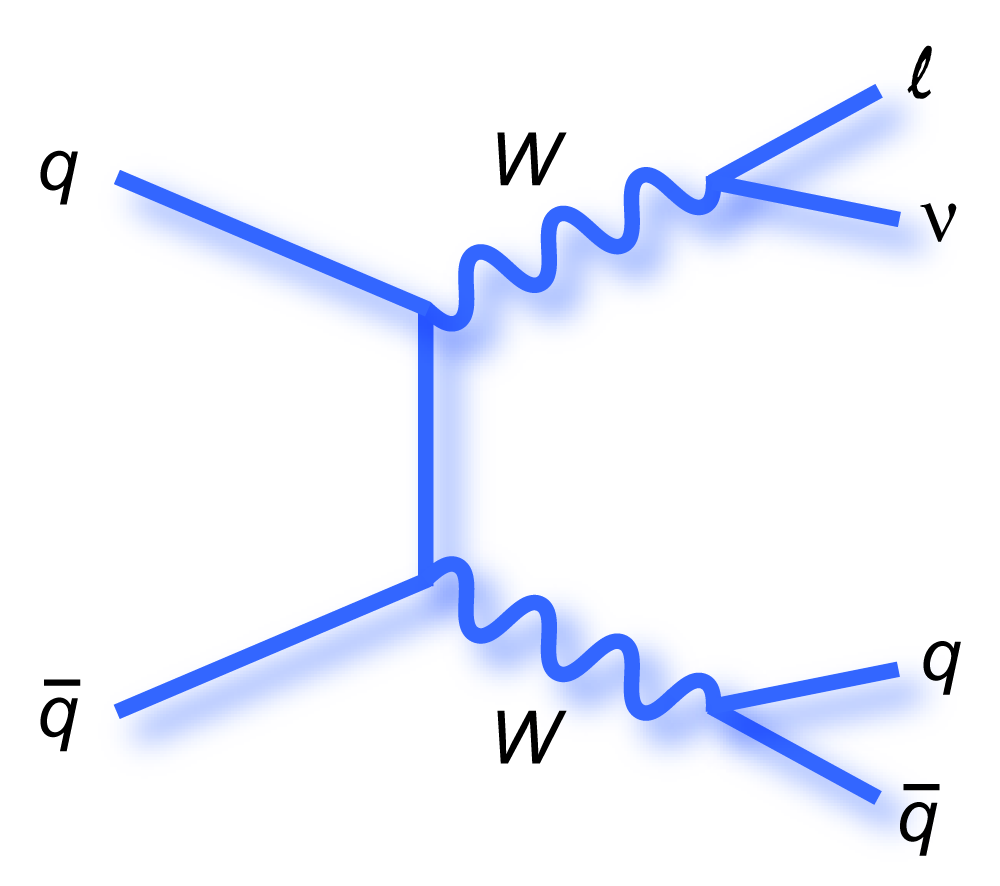
\includegraphics[width=0.49\textwidth]{lostlepton/plots/feynman_WW_lnuqq_bold_midblue.png}
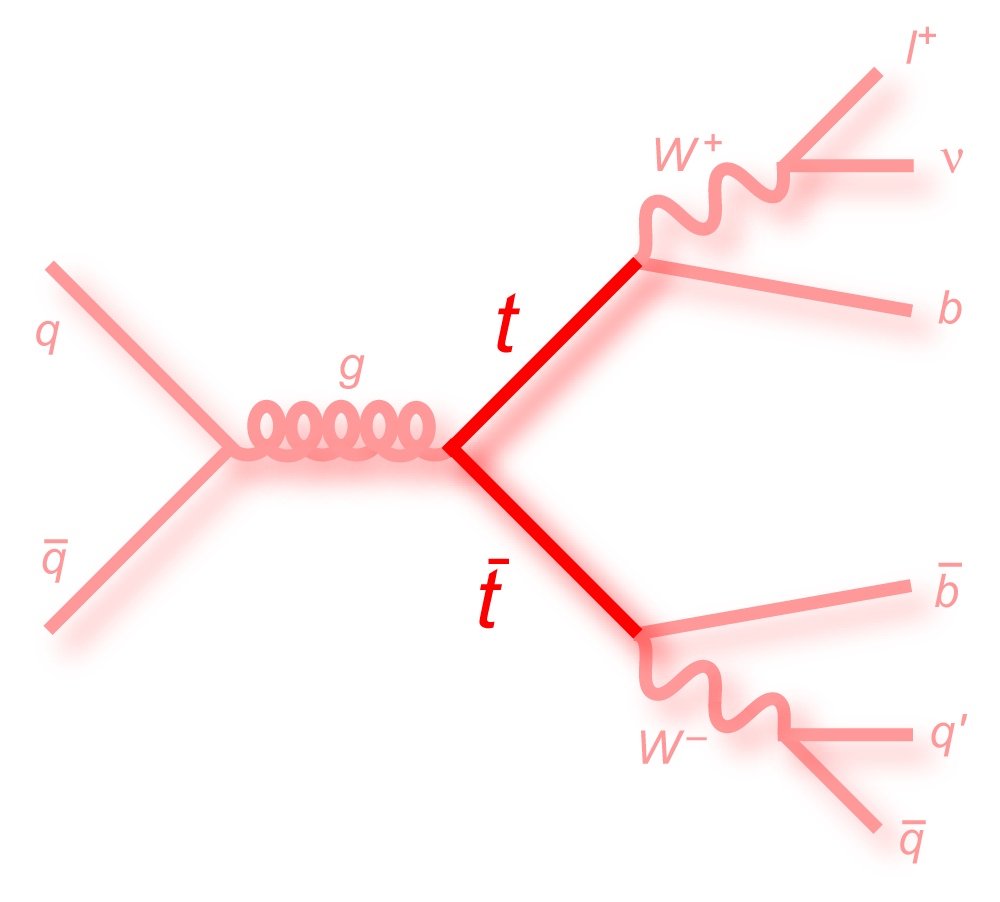
\includegraphics[width=0.49\textwidth]{lostlepton/plots/ttbar_feynman.png}\\
\end{tabular}
\end{center}
\caption{Feynman diagram for a typical \wpj decay on the left and a \ttbar decay on the right at the LHC\cite{tevatronPlots:2010}.}
\label{fig:lostlepton_feynman}
\end{figure}
The $\nu$ leaves the detector undetected leading to missing transverse energy. The lepton veto defined in Sec.~\ref{sec:event_selection} removes only events if leptons are within the detectors acceptance and fulfill the reconstruction and isolation criteria. The lost-lepton background arises when the lepton veto fails to identify a prompt lepton.\\
%The method which is described in this section is capable of predicting events with lost leptons, for very high \HT and \MHT regions. 
The background is estimated by a muon control sample (CS) which is reweighted according to the lepton identification (in)efficiency of the detector.
%The idea of predicting these lost-leptons is to selecting events which full fill the same kinematic cuts, except that they include exactly one well detected muon. This sample is called the control sample (CS), see Sec. \ref{sec:controlSample}. 
%The spectrum of the $\mu$ CS \pt is compared for the simulated events to the muons selected on data. Good agreement can be observed. The \pt of the muon also adds to the \HT and \MHT.
%The \pt of the muon, which can be seen in plot\ref{fig:CSmuonpt}, adds to the \HT and \MHT.\\
%The events of the CS are re weighting according to the (in)efficiency of the detector to reconstruct leptons. 
This idea holds when the event kinematics of the CS and the not detected leptons are similar, so that the background can be modeled by the CS. Extensive tests on simulated events have been performed to prove the methods capability of predicting lost leptons, see Sec.~\ref{sec:closure_test}.\\
All plots in this section labeled ''CMS Simulation'', ''CMS preliminary'' or ''CMS'' have been done by me, made public by CMS and can be found on the public twiki web page \cite{bib:TWiki:SUS12011}.

\section{The control sample}
\label{sec:controlSample}
The control sample (CS) includes events which pass the same kinematic cuts as the event selection (see Sec.~\ref{sec:event_selection}) but the lepton veto is inverted requiring exactly one well identified muon. The \pt of the muon is included in the \HT and \MHT calculation.\\
A small contribution comes from \ttbar decays to two leptons (dileptonic). These events enter the CS if only one lepton is lost. The case that one lepton is lost is twice as often than both are lost. The amount of lost leptons is therefore overestimated by a factor of two for the dileptonic decays. A selection on MC of events including one muon from dileptonic decays has been compared to the selection where two leptons are lost. The \mt cut discussed in Sec.~\ref{sec:event_selection} reduces the amount of dileptons in the CS to only 3\% of the total CS. These 3\% lead to an over-prediction of 1.5\% of the total prediction. The prediction is corrected for this.\\
Another minor contribution arises form diboson event and single top. The contribution has been found to be be less than 1.5\% of the total CS. This contribution is covered within the assigned uncertainty (see Sec.\ref{sec:uncertainties}).
Fig.~\ref{fig:CSmuonpt} and Fig.~\ref{fig:LostLepton_MuCS_data_MC} show the \pt, \HT and \MHT distribution of the CS selected from simulated \ttbar and \wpj events and data. Good agreement can be observed.
 %This proves that the assumption of no significant difference of the event kinematics between the CS to the lost lepton is reasonable. 

\begin{figure}[tbhn]
\label{fig:LostLepton_MuCS_data_MC}
\begin{center}
\begin{tabular}{c}
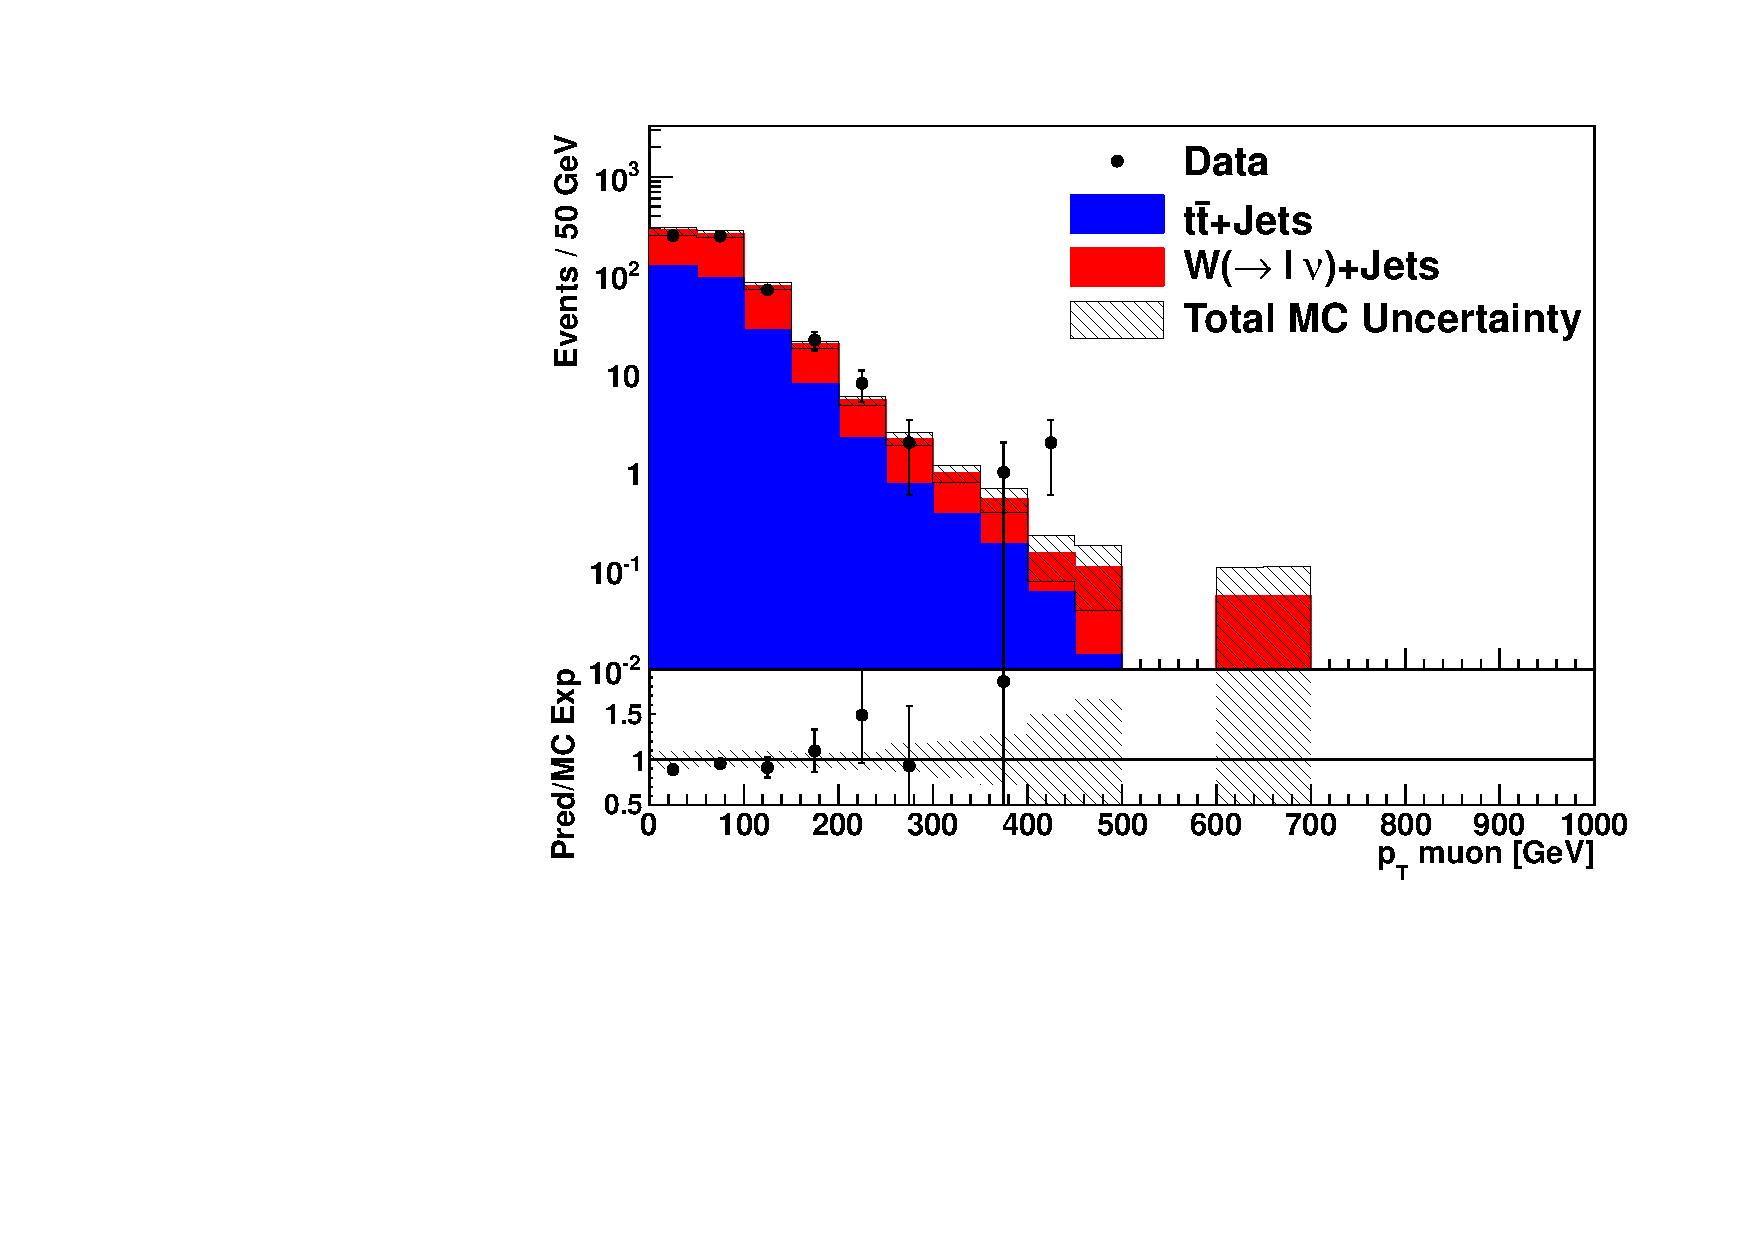
\includegraphics[width=0.90\textwidth]{lostlepton/plots/closure/CSMuonPT.pdf}
\end{tabular}
\end{center}
\caption{This plot shows a comparison of the $\mu$ control sample \pt spectrum selected on data corresponding to the full \lumi recorded 2011 and simulated \ttbar and \wpj events referred to as MC.}
\label{fig:CSmuonpt}
\end{figure}

\begin{figure}[tbhn]
\begin{center}
\begin{tabular}{cc}
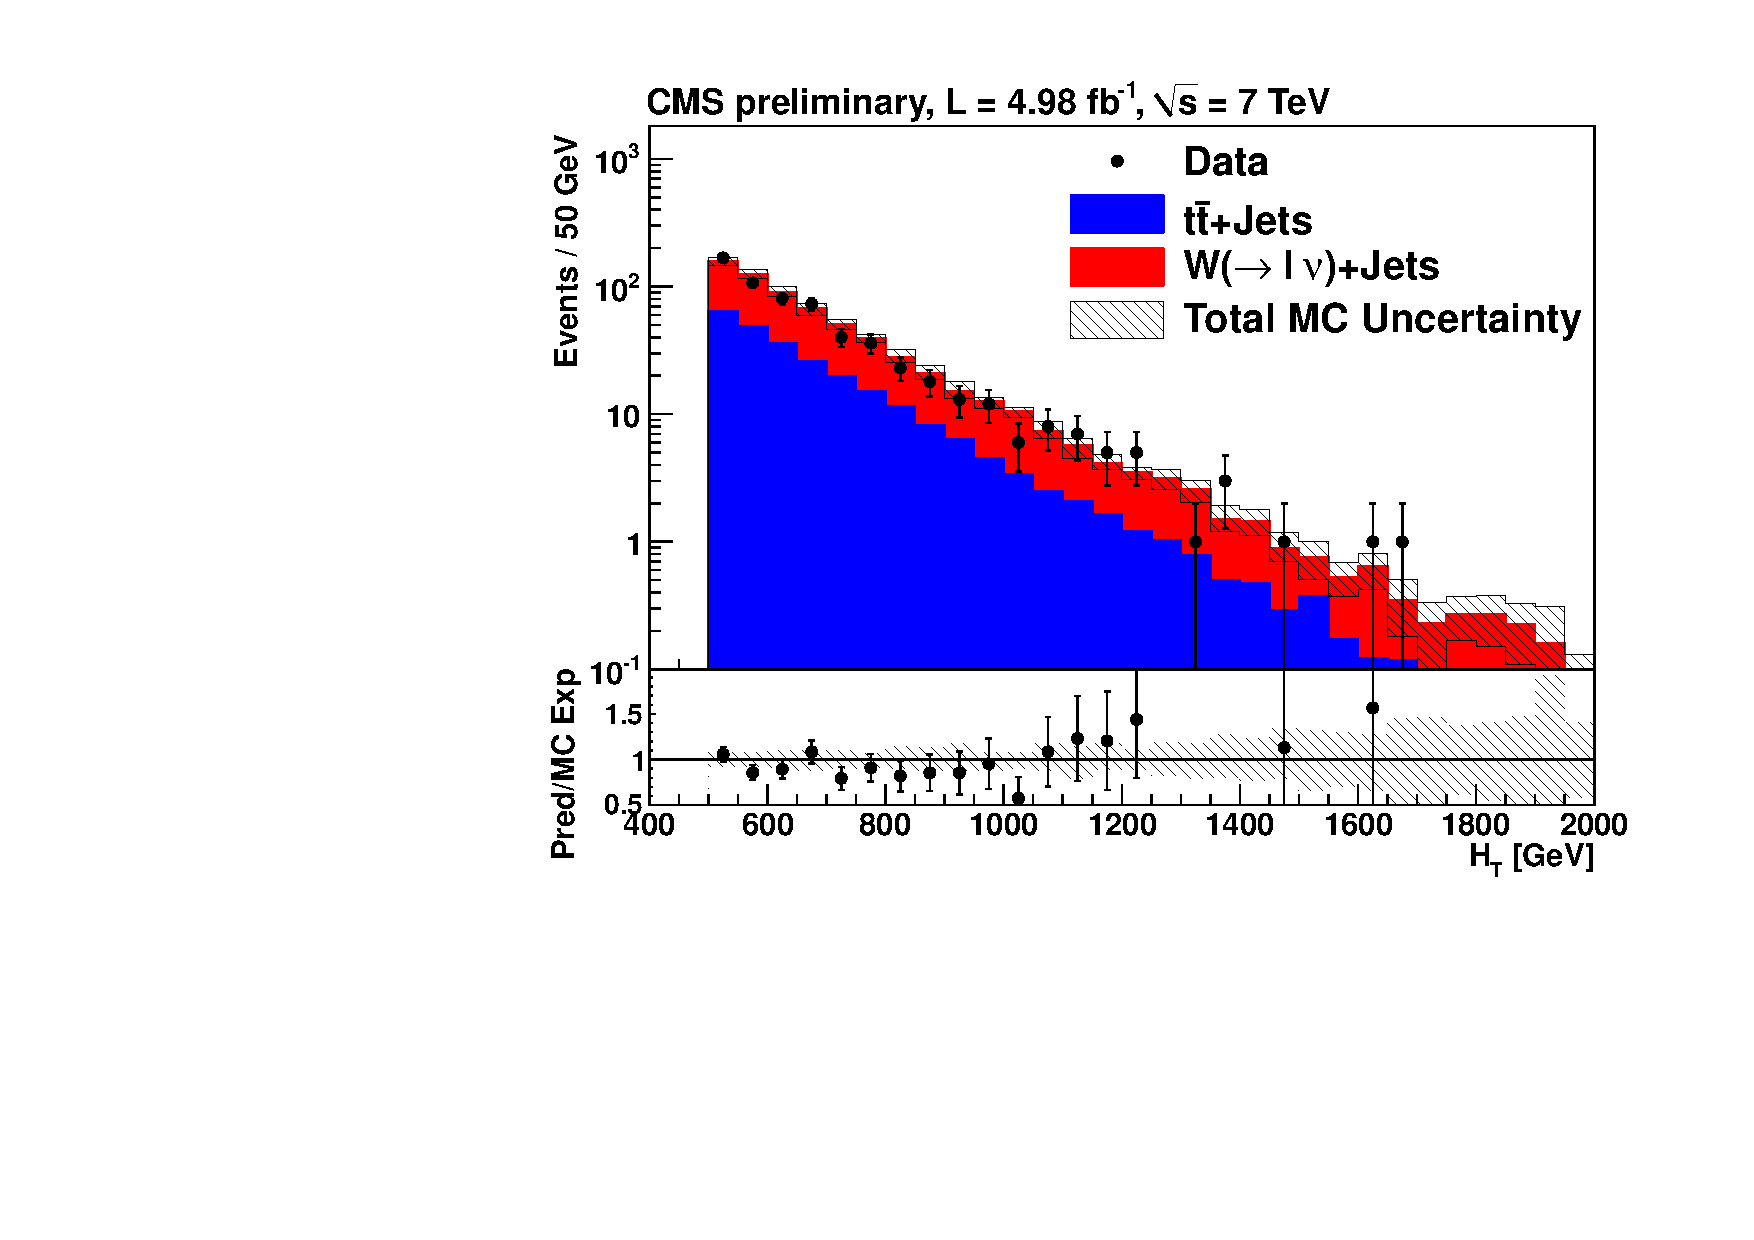
\includegraphics[width=0.9\textwidth]{lostlepton/plots/ANplots/Control_HT.pdf}\\
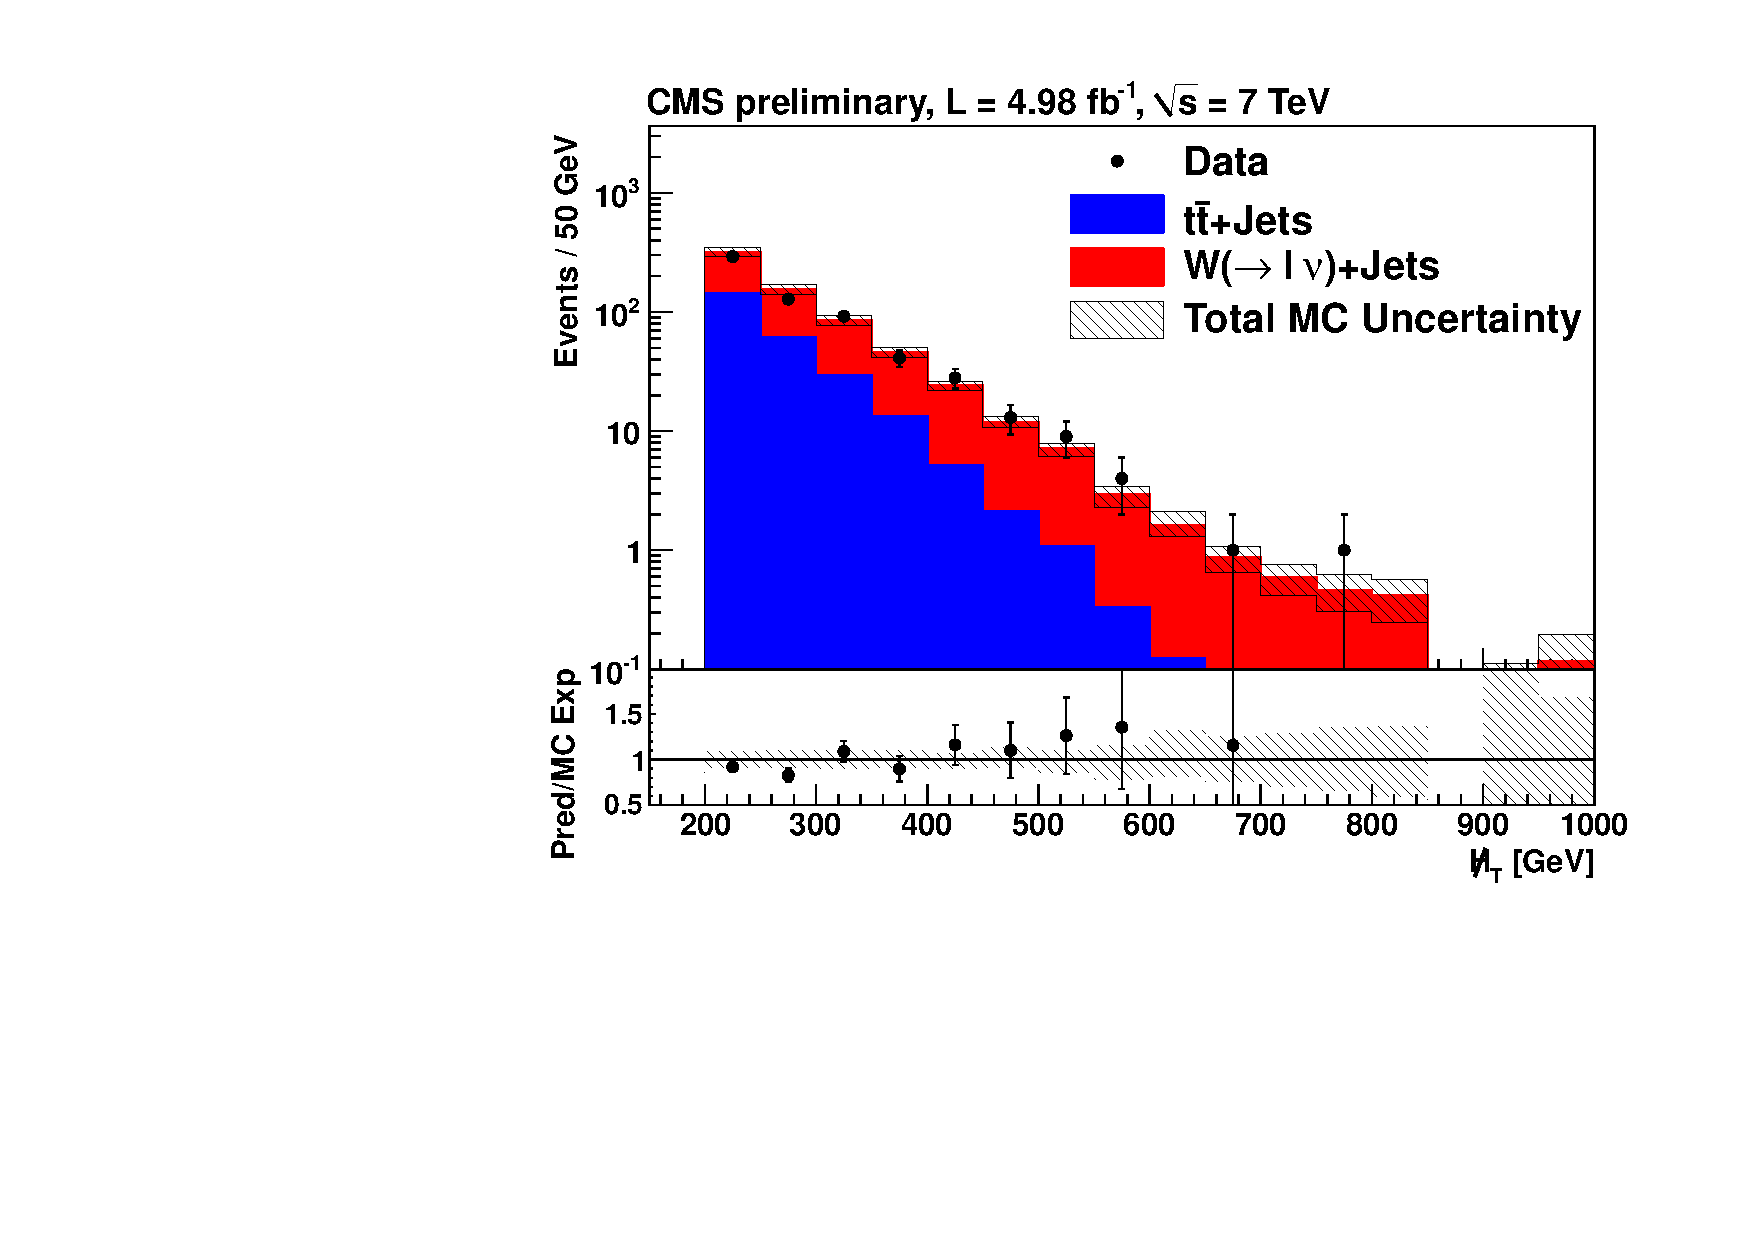
\includegraphics[width=0.9\textwidth]{lostlepton/plots/ANplots/Control_MHT.pdf}
%\includegraphics[angle=0,width=0.5\textwidth]{wtop_lostlepton_figures/MHTMHT_r}&
%\includegraphics[angle=0,width=0.5\textwidth]{wtop_lostlepton_figures/HTHT_r}
%%(a)&(b)\\
\end{tabular}
\end{center}
\caption{These figures show a comparison of the $\mu$ control sample for the \HT and \MHT distribution selected on data corresponding to the full \lumi recorded 2011 and simulated \ttbar and \wpj events.}

\end{figure}

% Data-MC comparison


\clearpage


\subsection{Signal Contamination}
\label{sec:signal_contamination}
Events involving physics beyond the standard model can contain jets, missing transverse momentum and leptons, in particular muons in the final state. Such events can enter the CS leading to an over estimation of the lost-lepton background. This is referred to as ''signal contamination'' of the CS.\\ 
For the SM background the muons in the CS are products of a \W decay while this is generally not expected for signal events. The topology of the \W decay can be used to distinguish between SM background and signal events.
The transverse-mass-distribution (\mt) has shown to be a useful value to remove possible signal contamination of the CS.\\

 \begin{equation}
 m_{T} = \sqrt{2 p_{T}(\mu) \met (1 - \cos(\Delta \Phi))}
\label{eq:mt}
\end{equation}
with $p_{T}(\mu)$ being the \pt of the muon in the CS, $\hspace{1mm} \met$ the missing energy in the event and $\Delta \Phi$ being the angel between the $\vec{\met}$ and the $\mu$.\\
\begin{figure}[tbhn]
\begin{center}
\begin{tabular}{c}
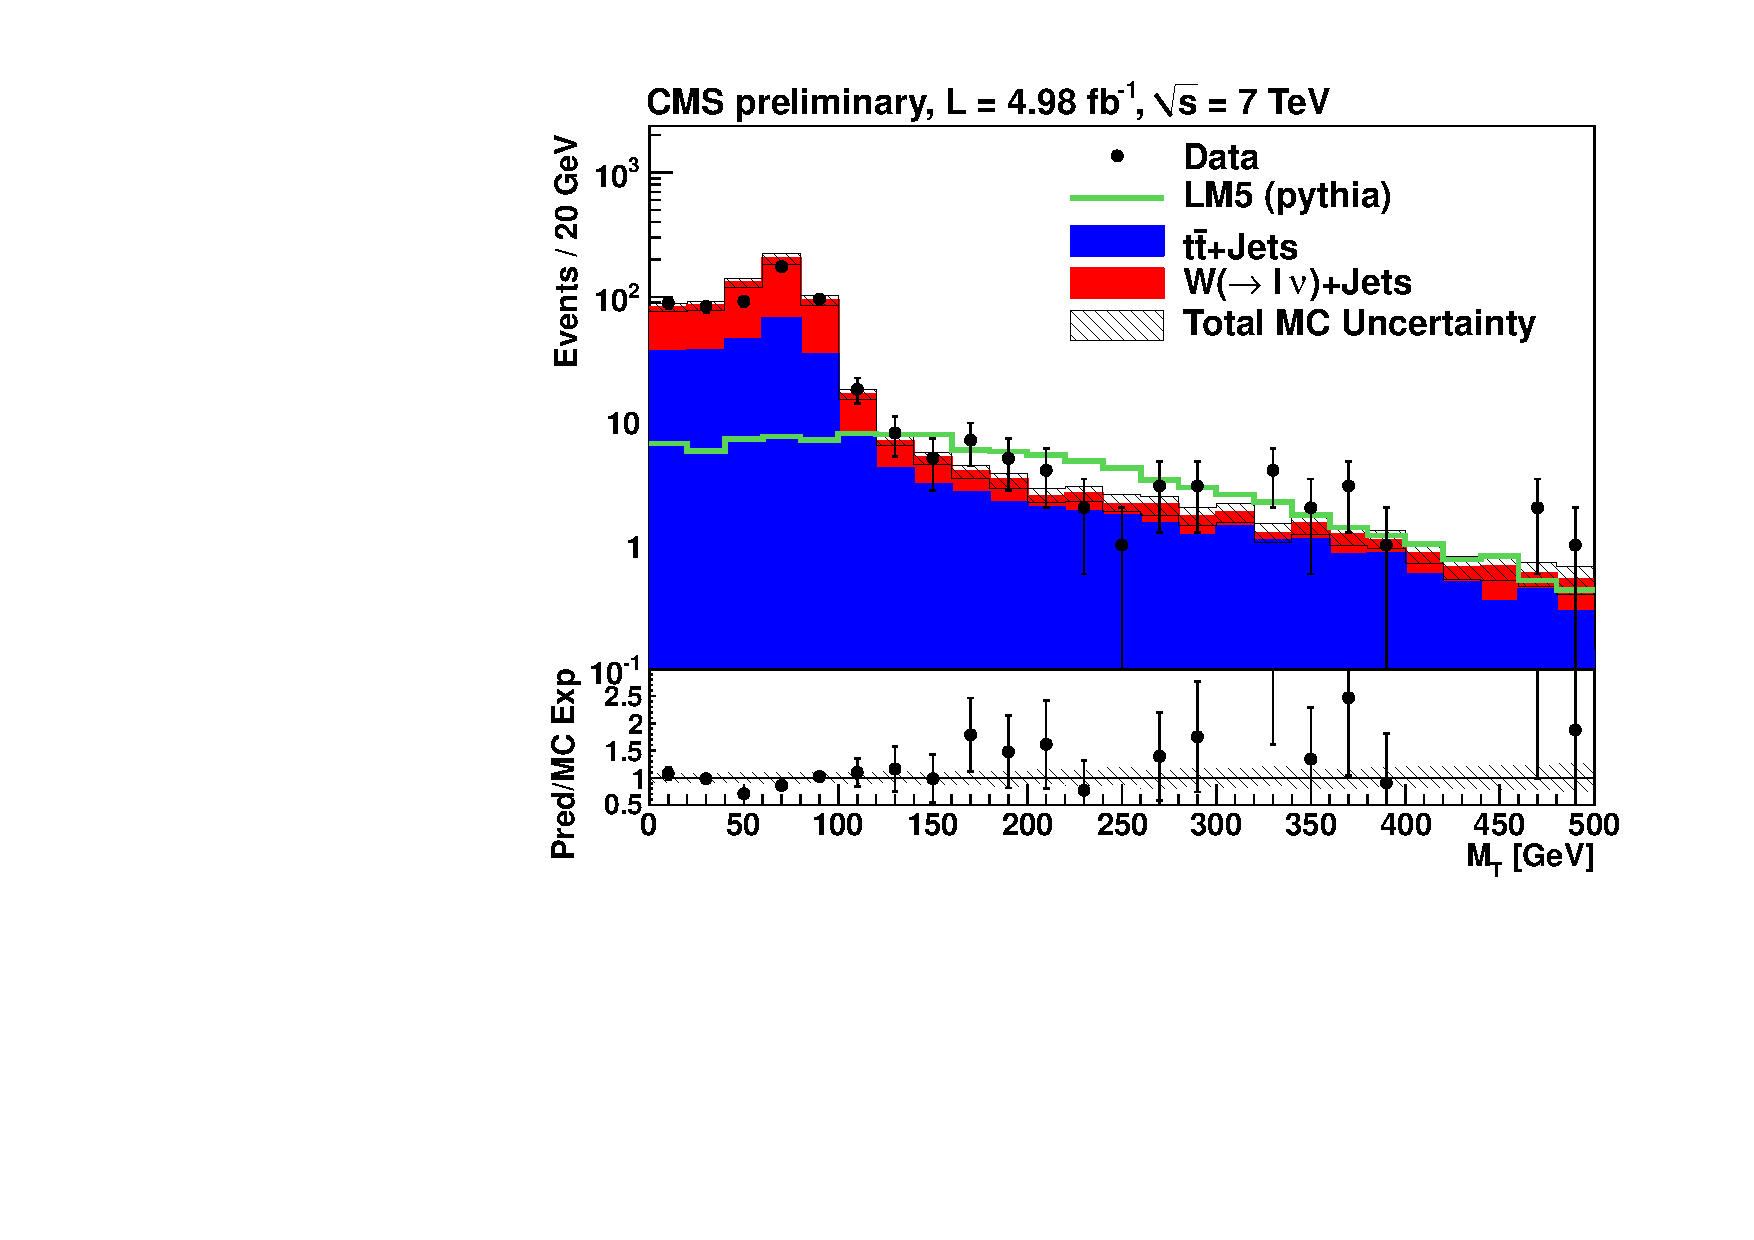
\includegraphics[width=1\textwidth]{lostlepton/plots/ANplots/Control_MTW.pdf}\\
\end{tabular}
\end{center}
\caption{This plot shows the \mt distribution of the control sample in data, for simulated \ttbar and \wpj events and for an example signal point (LM5). The \mt distribution of the CS steeply falls above $80 \gev$ for the SM process, where as the LM5 distribution is rather wide. (The legend description can be found in the caption of Fig.~\ref{fig:LostLepton_MuCS_data_MC})}
\label{fig:control_mtw}
\end{figure}
Fig.~\ref{fig:control_mtw} shows the \mt for the CS selected on data and MC together with the LM5 cMSSM benchmark point.
For the SM background events the transverse-mass-distribution rises up to the \w mass of 80.4 \gev above which it steeply falls while a broad distribution is being observed for signal events (LM5).\\
A cut at 100 \gev to remove everything above has shown a good balance between Standard Model CS reduction and signal contamination rejection. Note that because of the detectors finite resolution of muon and jet \pt some cases have a \mt value higher than $m_W$\footnote{Also the small amount of dileptonic \ttbar decays lead to higher \mt.}.\\
The efficiency, defined as the ratio of Standard Model CS events passing the cut to all Standard Model CS events, for the search regions and the baseline selection can be seen in Fig.~\ref{fig:mt_cut_eff}. The error bars cover the statistical uncertainty of the used MC. A good efficiency of about 90\% can be observed for all regions.\\
A constant correction factor of 10\% together with an uncertainty of 4.0\% is applied on data to correct for the removed Standard Model CS and cover for the variation of the cut efficiency.\\
Overall, possible signal contamination leading to an over estimation of the background and therefore a reduction of the sensitivity of the analysis to new particles has been reduced by the \mt cut, increasing the capability of the analysis of finding new physics.
\begin{figure}[tbhn]
\begin{center}
\begin{tabular}{c}
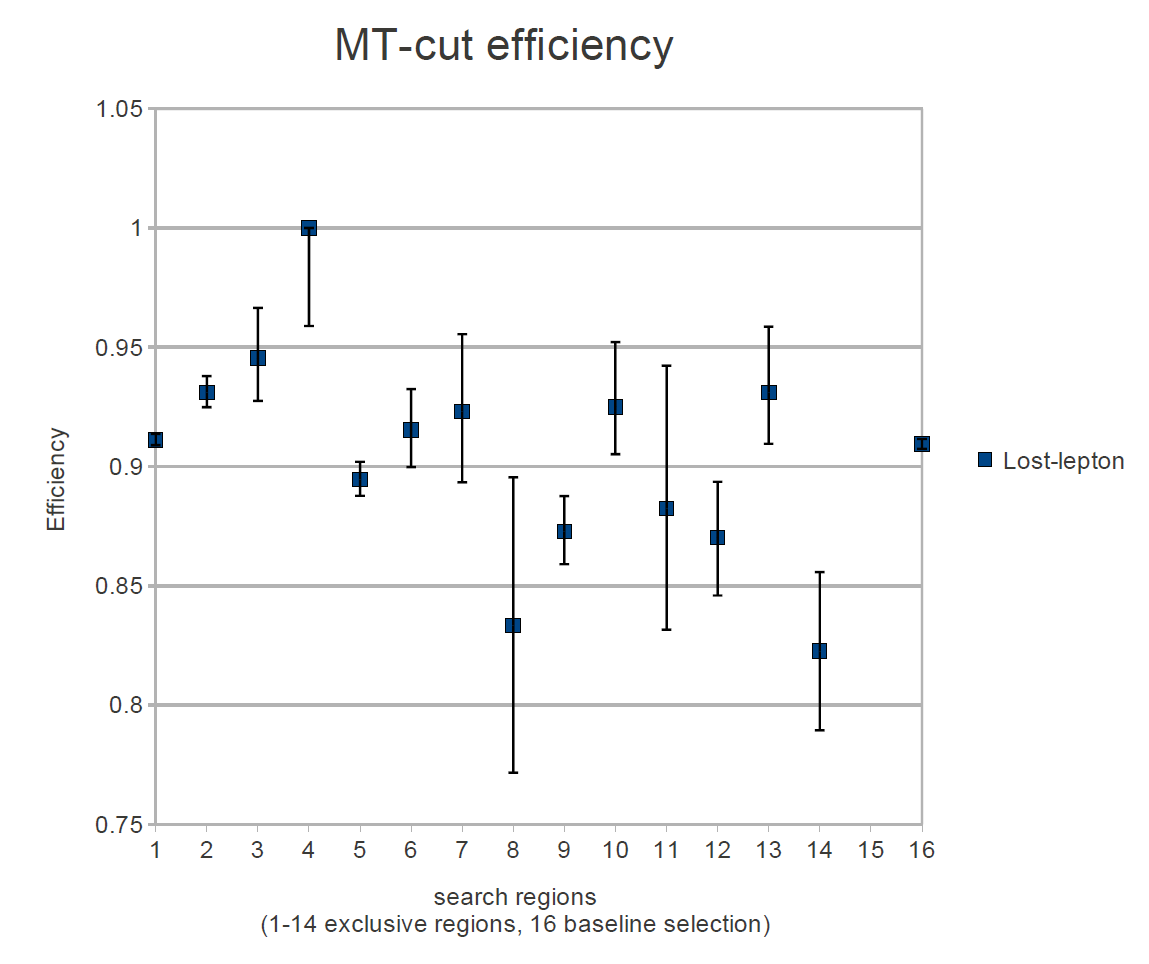
\includegraphics[width=1\textwidth]{lostlepton/plots/MT_eff.png}\\
\end{tabular}
\end{center}
\caption{This plot shows the efficiency of the $\mt$ cut for all exclusive regions (the numbering corresponds to the enumeration in Tab.\ref{tab:regions}) for bin 1-14. Bin 16 shows the value for the baseline selection. }
\label{fig:mt_cut_eff}
\end{figure}



% used in the selection by rejecting events with a reconstructed \W mass above 100 \gev. The removed CS amount which is above 100 \gev is being corrected for. Fig. \ref{fig:mt_LM5_baseline} shows the \mt distribution for the baseline selection of the CS and an example SUSY signal point.\\

%It is possible to calculate from the decay products, namely the muon and the $\met$ from the neutrino the transverse component of the \W mass. The muon is being reconstructed with its angel $\phi$, $\eta$ and \pt. The \met comes ideally from the not detected $\nu$. The combination of $\Delta \phi$ between the $\met$ and the muon together with the \pt of the muon and the $\met$ represents the ''transverse mass'' \mt of the decaying particle. 
% \begin{equation}
% m_{T} = \sqrt{2 p_{T}(\mu) \slash \met (1 - \cos(\Delta \Phi))}
%\label{eq:mt}
%\end{equation}
%The transverse-mass-distribution rises up to the \w mass of 80 \gev above which it steeply falls. Since the detector has a finite resolution of the muon \pt and jets are measured with an uncertainty on the energy \mt reconstructed higher than 80 \gev are expected. The cut is applied at 100 \gev to keep the reduction of the CS small. Studies have been done for different \HT and \MHT cuts on MC comparing the amount of muons passing and failing the \mt cut to evaluate the \mt cut correction factor. The resulting $\mt$ cut efficiencies can be seen in fig.\ref{fig:mt_cut_eff}. The error bars cover the statistics of the MC where positive error bars show Poisson errors while Gaussian error bars are used for the negative errors. A constant correction factor of 10\% for all regions is justified combined with the statistical uncertainty of the cut efficiencies and the assigned uncertainty of 43\% on the cut.\\
%Outliers are coming from mis-measurements of the muon \pt and the jets or from dileptonic \ttbar decays. These fraction of the CS is being removed by the $\mt$ cut. .\\
%For events where the $\met$ is caused by, for example, a LSP the cut becomes more efficient for higher \HT and \MHT selections since the \mt coming from LSPs is broadly distributed, as can be seen for the baseline selection in fig. \ref{fig:mt_LM5_baseline}.\\



 






\subsection{Other SM background contributions}
\label{sec:other_sm_contribution}
The main SM background contributing to lost-lepton CS arises as discussed from \ttbar and \wpj events. However other processes can contribute by ending up in the CS. There are QCD events, $ZZ$ or $Z$  processes which can have the same signature and contribute to the background.\\
The samples listed in Tab.~\ref{tab:MC_samples} have been used to study these backgrounds by selecting a control sample on the corresponding MC samples.
Tab.~\ref{tab:other_sm_contribution} shows the amount of events for each of the other SM backgrounds scaled to the full luminosity of \lumi. No considerable amount of events has been found. An uncertainty of less than $3\%$ is justified to cover for these SM background contributions and for possible other contributions which are expected to be magnitudes below the listed ones.

\begin{table}[htb]
\begin{center}
    \begin{tabular}{|l|l|l|l|}
        \hline
			& Number of Events in the CS 	& $\pm$         & ratio[\%]	\\  \hline
        $QCD$ 		&0 				& 0 		&0		\\ 
        $ZZ$   		&0.04  				& 0.02		&0.0	 	\\
        $Z$    		&7.99  				& 2.02		&1.2 		\\ 
        $Summe$ 	&8.03				& 2.04		&1.2 		\\ \hline
	\wpj \& \ttbar 	& 658.20	&5.00  & 100   \\ 
%        \ttbar &  --	   & ---     \\
        \hline

    \end{tabular}
\caption{This table shows the amount of additional SM processes which add to the CS selected on MC compared to the selection from \ttbar and \wpj events. The shown ratio is defined as SM background divided by the main background (\ttbar and \wpj). All numbers are scaled to the full luminosity of \lumi .\label{tab:other_sm_contribution}}
\end{center}


\end{table}

\clearpage






\section{Predicting the lost electrons and muons}
\label{sec:ll_prediction}
% sketch of the control sample
\begin{figure}[tbhn]
\begin{center}
\begin{tabular}{c}
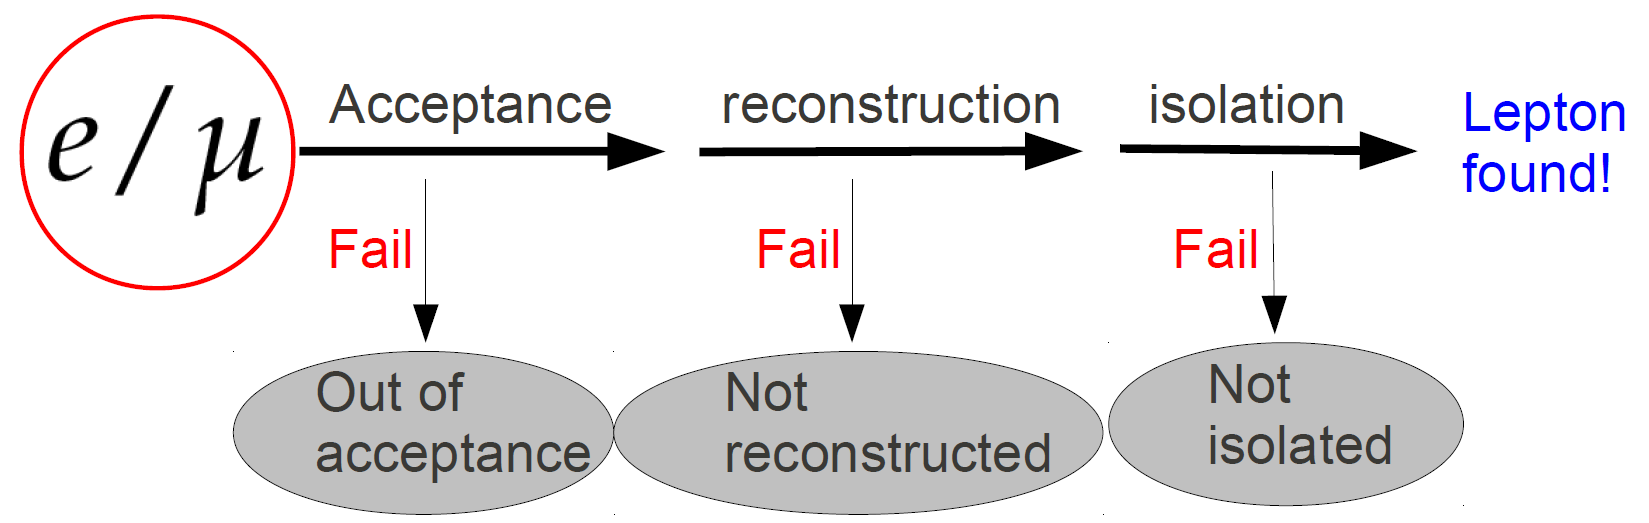
\includegraphics[width=0.80\textwidth]{lostlepton/plots/lepton_veto_sketch.png}\\
\end{tabular}
\end{center}
\caption{Visualization of the steps a muon has to take in order to enter the control sample}
\label{fig:sketch_lepton_veto}
\end{figure}
There are three steps a lepton has to take to be rejected by the lepton veto.
\begin{enumerate}

 \item First it has to be within the detector acceptance. 
 \item The second step is the reconstruction. 
 \item The final step is the isolation criteria.
\end{enumerate}
The CS is weighted according to each efficiency individually. 
Fig.~\ref{fig:sketch_lepton_veto} shows a chart of this three steps.\\
Since the control sample of well identified and isolated muons is used, one has to start predicting the three steps in reversed order.\\
Starting with modeling the not isolated muons followed by predicting the not reconstructed and finally the out of acceptance muons.
To model the not isolated muons the CS is weighted according to:
\begin{equation}
 \rm !ISO^{\mu} = {\rm CS}\cdot \frac{1-\epsilon_{\rm ISO}^{\mu}}{\epsilon_{\rm ISO}^{\mu}} 
    %%   \rm !ISO^{\mu}} = {\rm CS}\cdot \frac{1-\epsilon_{\rm ISO}^{\mu}}{\epsilon_{\rm ISO}^{\mu}} 
\label{eq:isolation_muon}
\end{equation}
with $\rm !ISO^{lepton}$ being the applied weight and $\epsilon_{X}^{\mu/e}$ being the efficiency of the criteria $X$ for the lepton.\\
The next step is to model the not reconstructed muons which is done by taking the muon isolation and reconstruction (in)efficiency into account. The weight is calculated according to the following equation:
\begin{equation}
 {\rm !Reco^{\mu}} = {\rm CS}\cdot \frac{1}{\epsilon_{\rm ISO}^{\mu}} \cdot \frac{1-\epsilon_{\rm Reco}^{\mu}}{\epsilon_{\rm Reco}^{\mu}}
\label{eq:reconstruction_muon}
\end{equation}
The last step in modeling the lost muons is to take also the muons into account which fall out of the detector acceptance. The weight has to include the isolation and reconstruction (in)efficiencies together with the out of acceptance efficiency:
\begin{equation}
 {\rm !Acc^{\mu}} = {\rm CS}\cdot \frac{1}{\epsilon_{\rm ISO}^{\mu}}\cdot \frac{1}{\epsilon_{\rm Reco}^{\mu}} \cdot \frac{1-\epsilon^{\mu}_{Acc}}{\epsilon^{\mu}_{Acc}}
\label{eq:acceptance_muon}
\end{equation}
The electrons are modeled using the same muon CS. This is valid since the decay of a $W$ to a $\mu$ or $e$ has according to the lepton universality the same probability\cite{bib:berger}.
All muon (in)efficiencies need to be taken into account before modeling the lost electrons resulting in more complex equations. The following equations are used to model the not isolated (Eq.~\ref{eq:elec_iso}), not reconstructed (Eq.~\ref{eq:elec_reco}) and the out of acceptance electrons (Eq.~\ref{eq:elec_acc}). 
\begin{equation}
{\rm !ISO^{e}} = {\rm CS}\cdot \frac{1-\epsilon_{\rm ISO}^{e}}{\epsilon_{\rm ISO}^{\mu}} \cdot \frac{\epsilon^{e}_{Reco}}{\epsilon^{\mu}_{Reco}} \cdot \frac{\epsilon^{e}_{Acc}}{\epsilon^{\mu}_{Acc}}
\label{eq:elec_iso}
\end{equation}
\begin{equation}
{\rm !Reco^{e}} = {\rm CS}\cdot \frac{1}{\epsilon_{\rm ISO}^{\mu}}\cdot \frac{1-\epsilon_{\rm Reco}^{e}}{\epsilon_{\rm Reco}^{\mu}}  \cdot \frac{\epsilon^{e}_{Acc}}{\epsilon^{\mu}_{Acc}}.
 \label{eq:elec_reco}
\end{equation}
\begin{equation}
{\rm !Acc^{e}} = {\rm CS}\cdot \frac{1}{\epsilon_{\rm ISO}^{\mu}}\cdot \frac{1}{\epsilon_{\rm Reco}^{\mu}}  \cdot \frac{1 - \epsilon^{e}_{Acc}}{\epsilon^{\mu}_{Acc}}
 \label{eq:elec_acc}
\end{equation}

%\begin{equation}
%{\rm !ID^{e}} = {\rm CS}\cdot \frac{1}{\epsilon_{\rm ISO}^{\mu}}\cdot \frac{1-\epsilon_{\rm ID}^{e}{\epsilon_{\rm ID}^{\mu}}  \cdot \frac{\epsilon^{e}_{Acc}}{\epsilon^{\mu}_{Acc}}.
% \label{eq:elec_acc}
%\end{equation}
The final equation to predict all lost leptons is:
\begin{equation}
\label{eq:totalWeight}
 \text{all lost leptons} = C \cdot \sum_{i=e,\mu}\left(\text{!Iso}^i+\text{!Reco}^i+\text{!Acc}^i\right) 
\end{equation}
with $C$ being a correction factor consisting of the correction factor for the \mt cut efficiency discussed in Sec.~\ref{sec:signal_contamination}, a small factor for di-leptonic events discussed in Sec.~\ref{sec:controlSample} and a ''non-closure'' factor discussed in Sec.~\ref{sec:closure_test}.





\clearpage

\section{Lepton Efficiencies}
\label{sec:efficiencies}
This chapter describes how the six efficiencies, used to weighted the CS, are obtained.\\
The acceptance efficiency has been calculated from MC by comparing the amount of leptons fulfilling the acceptance criteria defined in Sec.~\ref{sec:acceptance} to all prompt leptons. This has been done for the baseline selection without the lepton veto for muons and electrons separately.\\
The isolation efficiencies, taken from \cite{bib:phd:jan}, were obtained by a Tag\&Probe method (Sec.~\ref{sec:tag_probe}) on the Z-Resonance. The efficiencies are parametrized in $\frac{p_{t,lep}}{p_{t,jet}}$, with $p_{t,lep}$ being the lepton and $p_{t,jet}$ being the \pt of the closest jet, and $\Delta R$ to the closest jet. \\
This is necessary since the lepton isolation depends strongly on the activity around the lepton (see Sec.~\ref{sec:event_selection}) and the selection of the $Z$-Resonance has a different topology than the topology of the signal.\\
The reconstruction efficiencies are obtained from MC by calculating the ratio of generator leptons which can be matched to reconstructed leptons.\\ %Other parametrization of the reconstruction efficiencies have been test including Tag\&Probe reconstruction efficiencies in $\eta$ and lepton \pt but they fail in accounting for the topological differences. Therefore the reconstruction efficiencies have to be obtained from MC. 
\subsection{Tag\&Probe method}
\label{sec:tag_probe}
Tag\&Probe methods are well established methods to measure the efficiency of detectors to identify and isolate leptons. The idea is to take a well known process which has a good understood final state of two leptons and good understood background processes (a fit function is used to model the background from other processes).\\
For the here presented efficiencies the $Z$-resonance was used. 
The $Z$-boson can only decay to two leptons, two jets or two neutrinos. Therefore if one lepton is found another lepton of the same flavor must be in the event too.\\
The Tag\&Probe method starts with a well identified ''tag''-lepton. The tag-lepton has to pass tight identification cuts to make sure that it is a proper prompt lepton.\\
To leave other possible leptons in the event unbiased this tag-leptons are required to fire the trigger used for the sample selection.\\
Then another lepton (''probe''-lepton) in the event is selected without any isolation and, depending on the to be probed efficiency, suitable reconstruction criteria. When this lepton is found both are combined to the mass of the $Z$-Boson. Only events with a reconstructed mass between 60 and 120 \gev for muons and 70 to  110 \gev for electrons are used.\\
Then the isolation criteria or reconstruction criteria are applied to the probe-lepton, resulting in a fraction of probe-leptons passing and failing the isolation criteria. A function to each fraction is fitted modeling the $Z$-resonance together with the other (exponentially decreasing) background events. The ratio of the integral of both signal fits are used as isolation efficiency. The fitting uncertainty is included in the efficiency as uncertainty (more details can be found here \cite{bib:phd:jan}). 




\subsection{Leptons out of the detector acceptance}
\label{sec:acceptance}
The out of detector acceptance leptons are defined as leptons with $\pt<10GeV$ and muons with a $|\eta|>2.4$ (electrons $|\eta|>2.5$) which can not be detected (see Sec.~\ref{sec:detector}). %In general the leptons coming from $\tau$ decays tend to have less \pt therefore are more often out of acceptance. 
For the high $\HT>500 \gev$ and $\MHT>200 \gev$ cuts the amount of leptons out of acceptance show no dependency on \HT or \MHT. For muons an acceptance efficiency of 84\% and for electrons 81\% has been found\footnote{The \HT and \MHT distribution for the out of acceptance leptons can be found in  Fig.\ref{fig:reco_acc_combined}.}. 

% This has been studied on MC and can be seen in \ref{fig:out_acceptance}.

%\begin{figure}[htbp]
%\begin{center}
%\begin{tabular}{cc}
%
\includegraphics[width=0.49\textwidth]{lostlepton/plots/FixMe.png}
%
\includegraphics[width=0.49\textwidth]{lostlepton/plots/FixMe.png}\\%%
%
%\end{tabular}
%\end{center}
%\caption{This figure shows the closure for muons out of acceptance in \HT and \MHT for \ttbar and \wpj combined. No trend for ether \HT nor \MHT can be observed.}
%\label{fig:out_acceptance}
%\end{figure}


%FIXME out of acceptance plot for HT MHT and Number of vertices.

\subsection{Not reconstructed leptons}
\label{sec:reconstruc}
For the reconstruction efficiencies of the electrons the Tag\&Probe method can not be used because the super clusters need to be cleaned by removing jets to have a significant purity of real electrons in the selection\cite{bib:phd:jan}.\\
In order to still use the same parametrization as for the isolation efficiencies the reconstruction efficiencies are obtained from MC. A conservative estimate of 9\% uncertainty is applied on the total prediction. In principle the $\mu$ could be calculated with the Tag\&Probe method.\\
Previously\cite{bib:phd:jan} the reconstruction efficiencies had been done with a Tag\&Probe method on data on the $Z$-Resonance with the parametrization of the efficiencies in $\frac{p_{t,lep}}{p_{t,jet}}$ and $\eta$. The prediction with the old efficiencies show a clear systematic under-prediction which is caused by the deficiency of the $\eta$ parametrization to account for the kinematic differences between the $Z$-Boson resonance and the search regions. \\ 
As explained above (see Sec.~\ref{sec:efficiencies}) it is not possible to use a parametrization as a function of $\Delta R$ to the closest jet in the Tag\&Probe method for the electrons, forcing the use of MC.\\
Fig.~\ref{fig:oldReco} shows a comparison of the closure tests for the prediction with the old efficiencies (right) and the new  prediction (left). A clear under-prediction can be observed for the old efficiencies while the new efficiencies show a very good closure.\\
Fig.~\ref{fig:reco_eff} shows the used electron and $\mu$ reconstruction efficiencies.

% old reco
\begin{figure}[tbhn]
\begin{center}
\begin{tabular}{c}
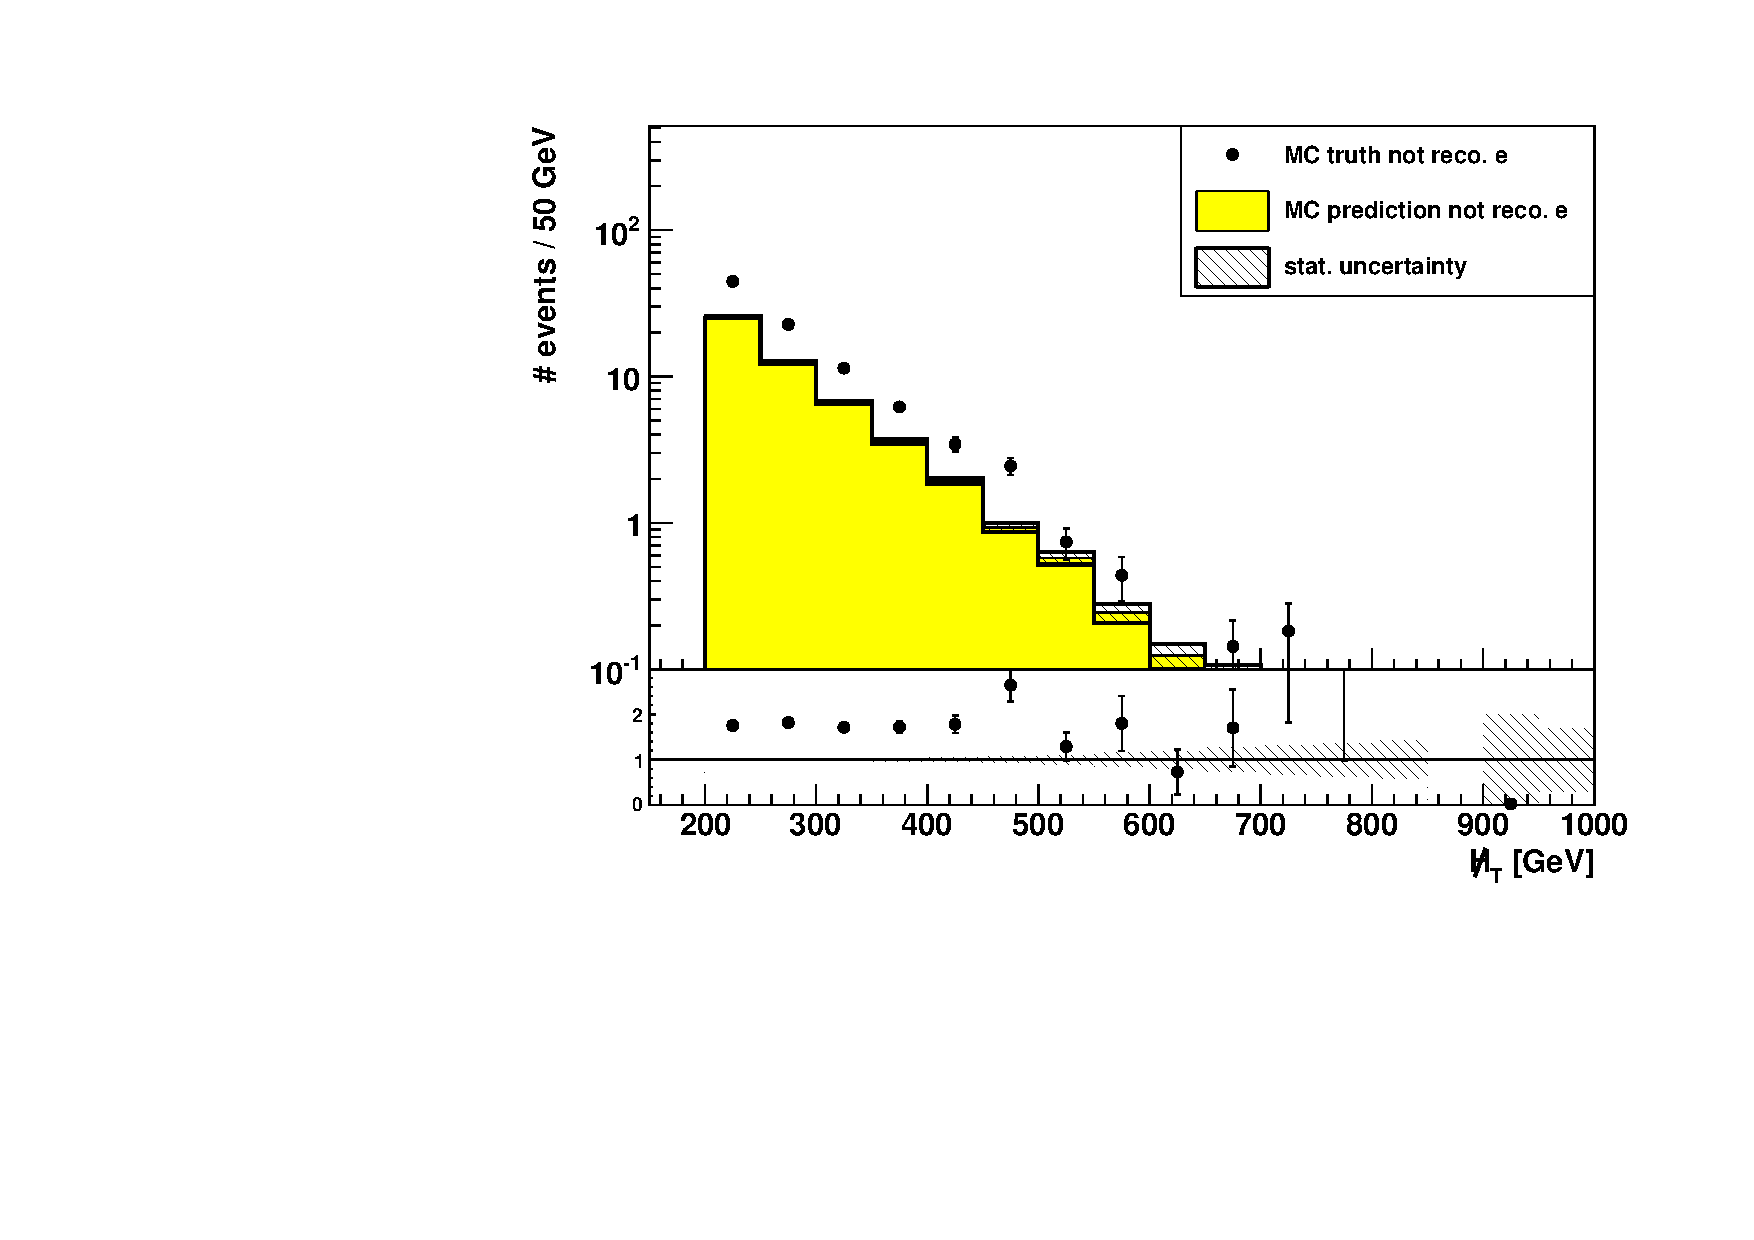
\includegraphics[width=.55\textwidth]{lostlepton/plots/MHTOldRecoE.pdf}
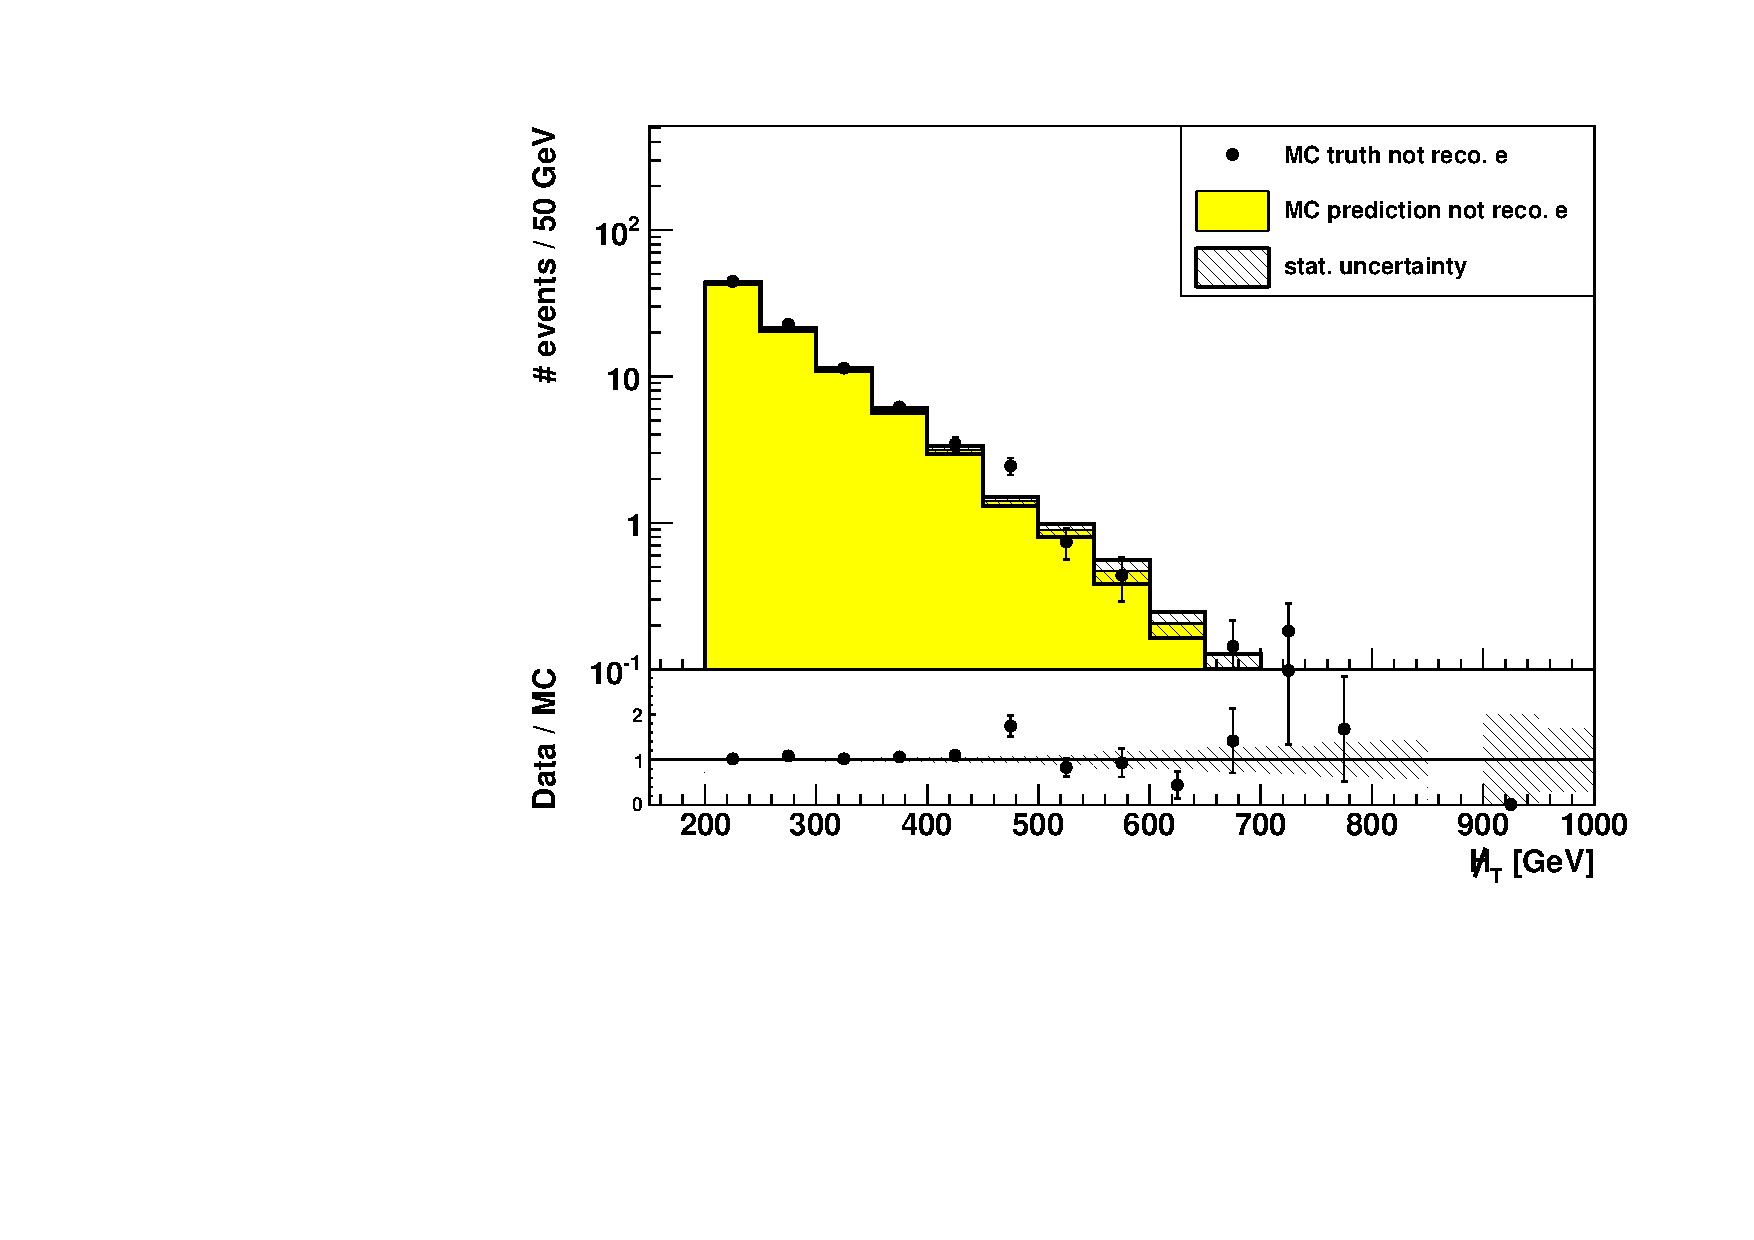
\includegraphics[width=.55\textwidth]{lostlepton/plots/MHTNewRecoE.pdf}\\
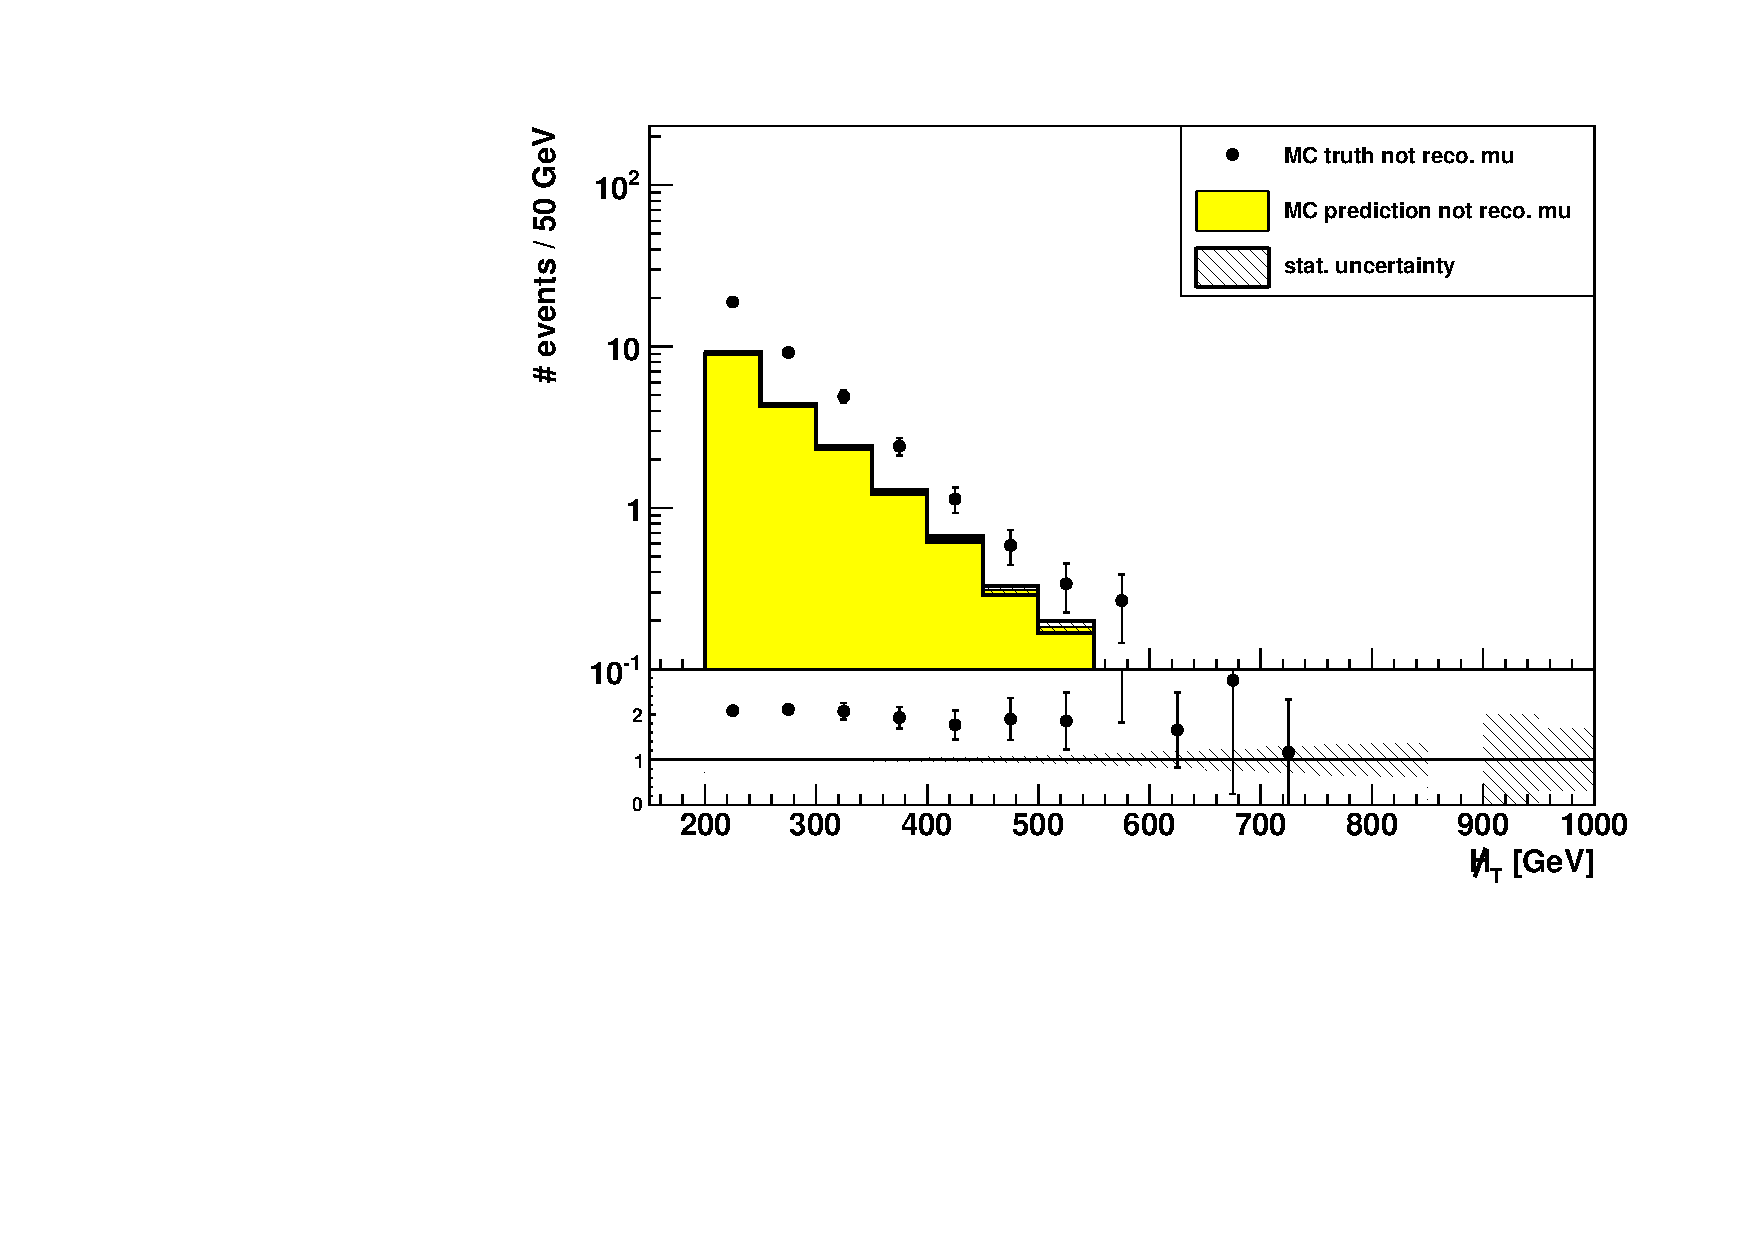
\includegraphics[width=.55\textwidth]{lostlepton/plots/MHTOldRecoMu.pdf}
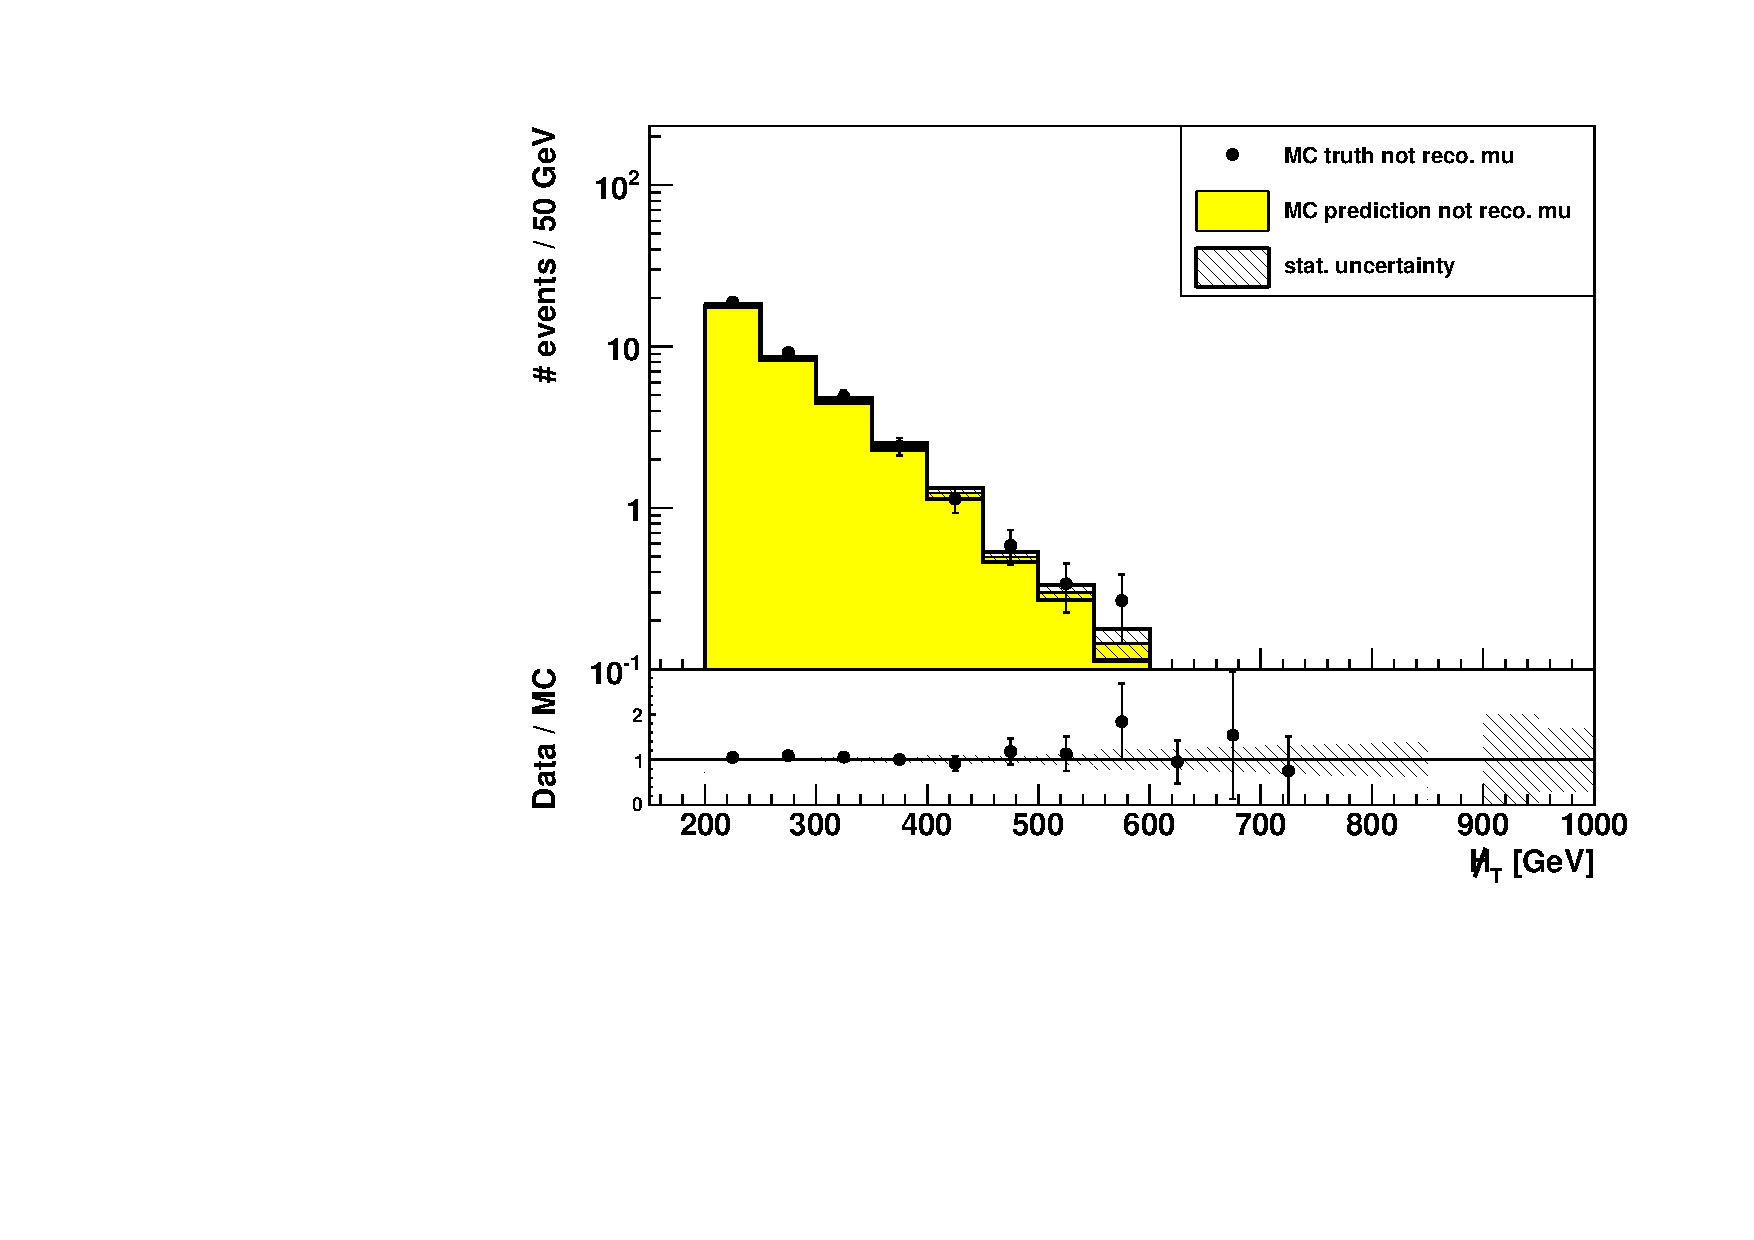
\includegraphics[width=.55\textwidth]{lostlepton/plots/MHTNewRecoMu.pdf}\\
%\includegraphics[angle=0,width=0.5\textwidth]{wtop_lostlepton_figures/MHTMHT_r}&
%\includegraphics[angle=0,width=0.5\textwidth]{wtop_lostlepton_figures/HTHT_r}
%%(a)&(b)\\
\end{tabular}
\end{center}
\caption{These plots show the MC closure (\ttbar and \wpj combined) for not reconstructed electrons (upper two plots) and muons (lower two plots). On the left side for the old efficiencies binned in $\frac{p_{t,lep}}{p_{t,jet}}$ and $\eta$ and on the right side with the new in lepton \pt and $\Delta R$ binned efficiencies.}
\label{fig:oldReco}
\end{figure}



%%% add 4 figures for not reco mu e ttbar and w separated
% iso eff
\begin{figure}[tbhn]
\begin{center}
\begin{tabular}{c}
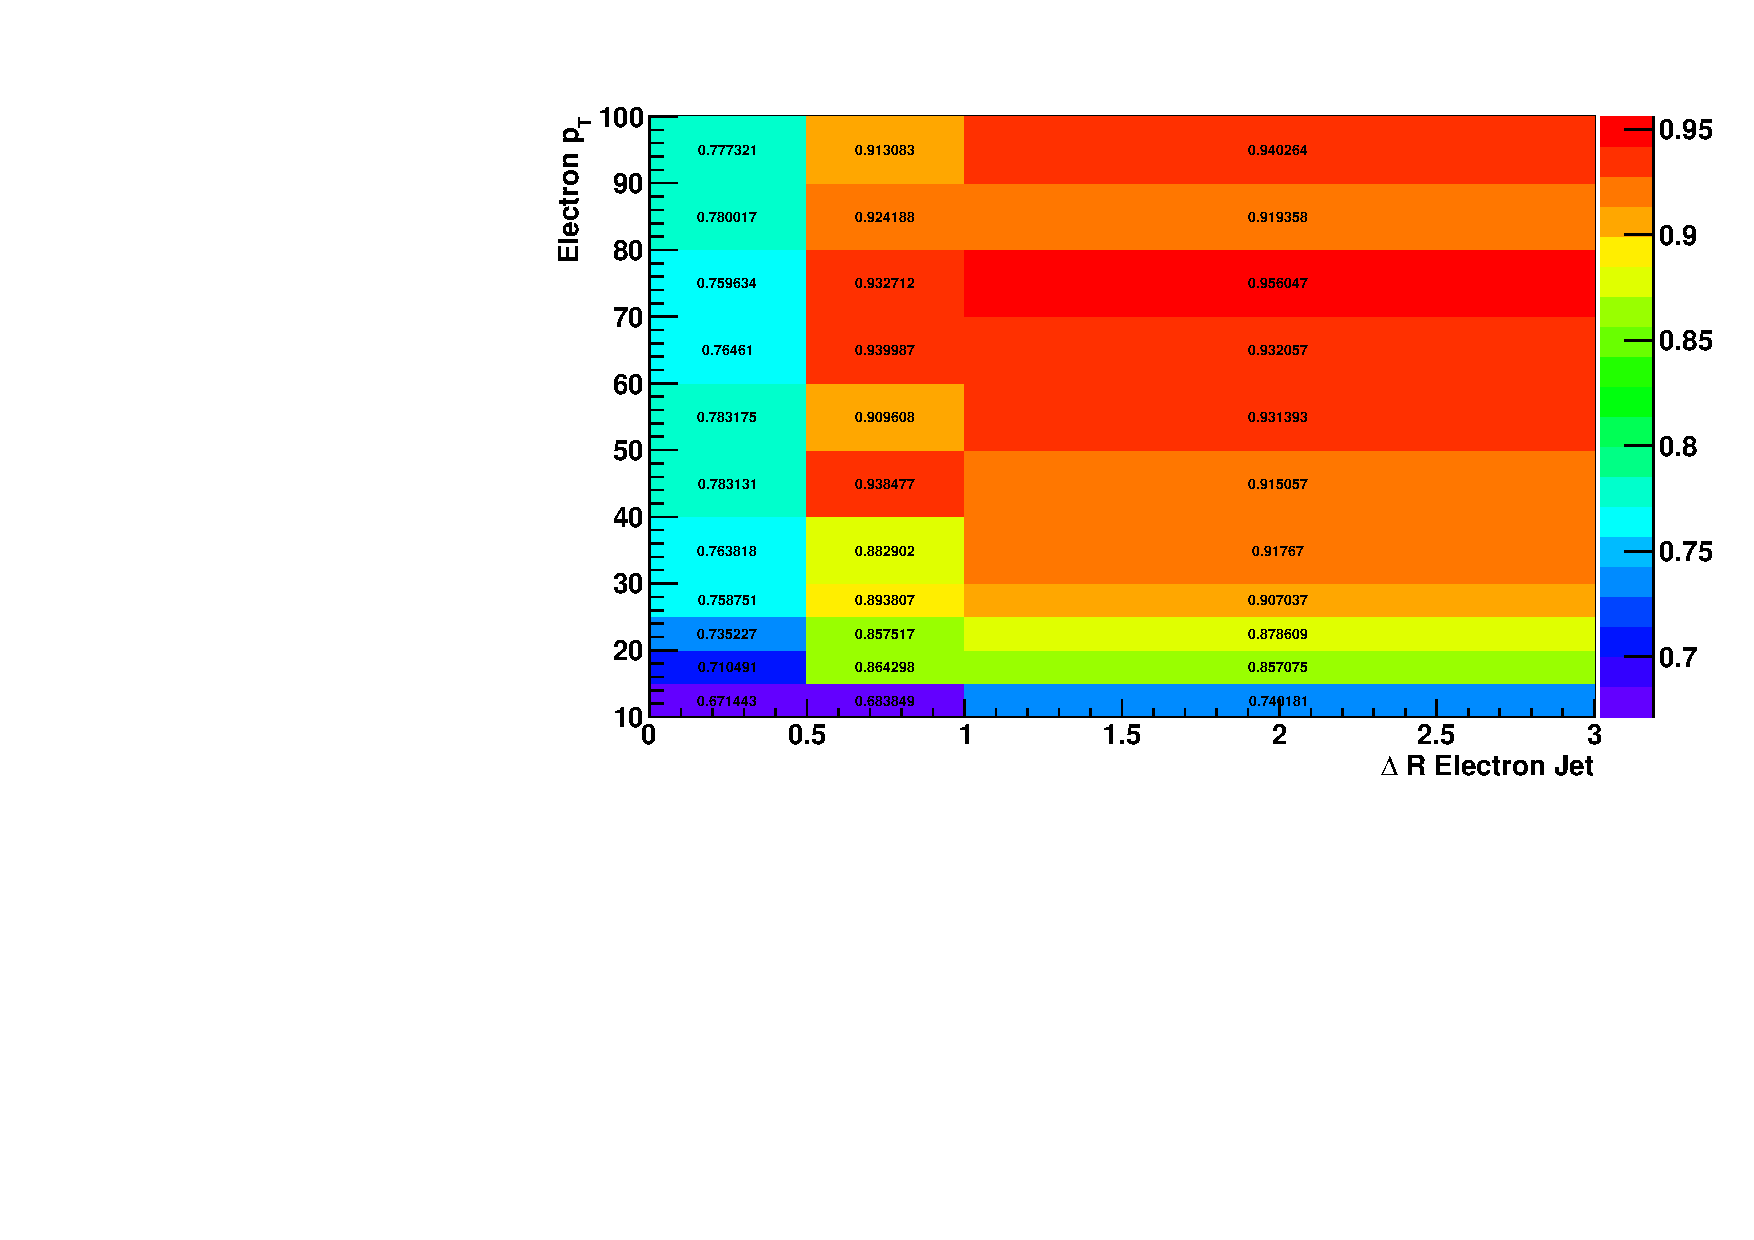
\includegraphics[width=.90\textwidth]{lostlepton/plots/Elec_Reco.pdf}\\
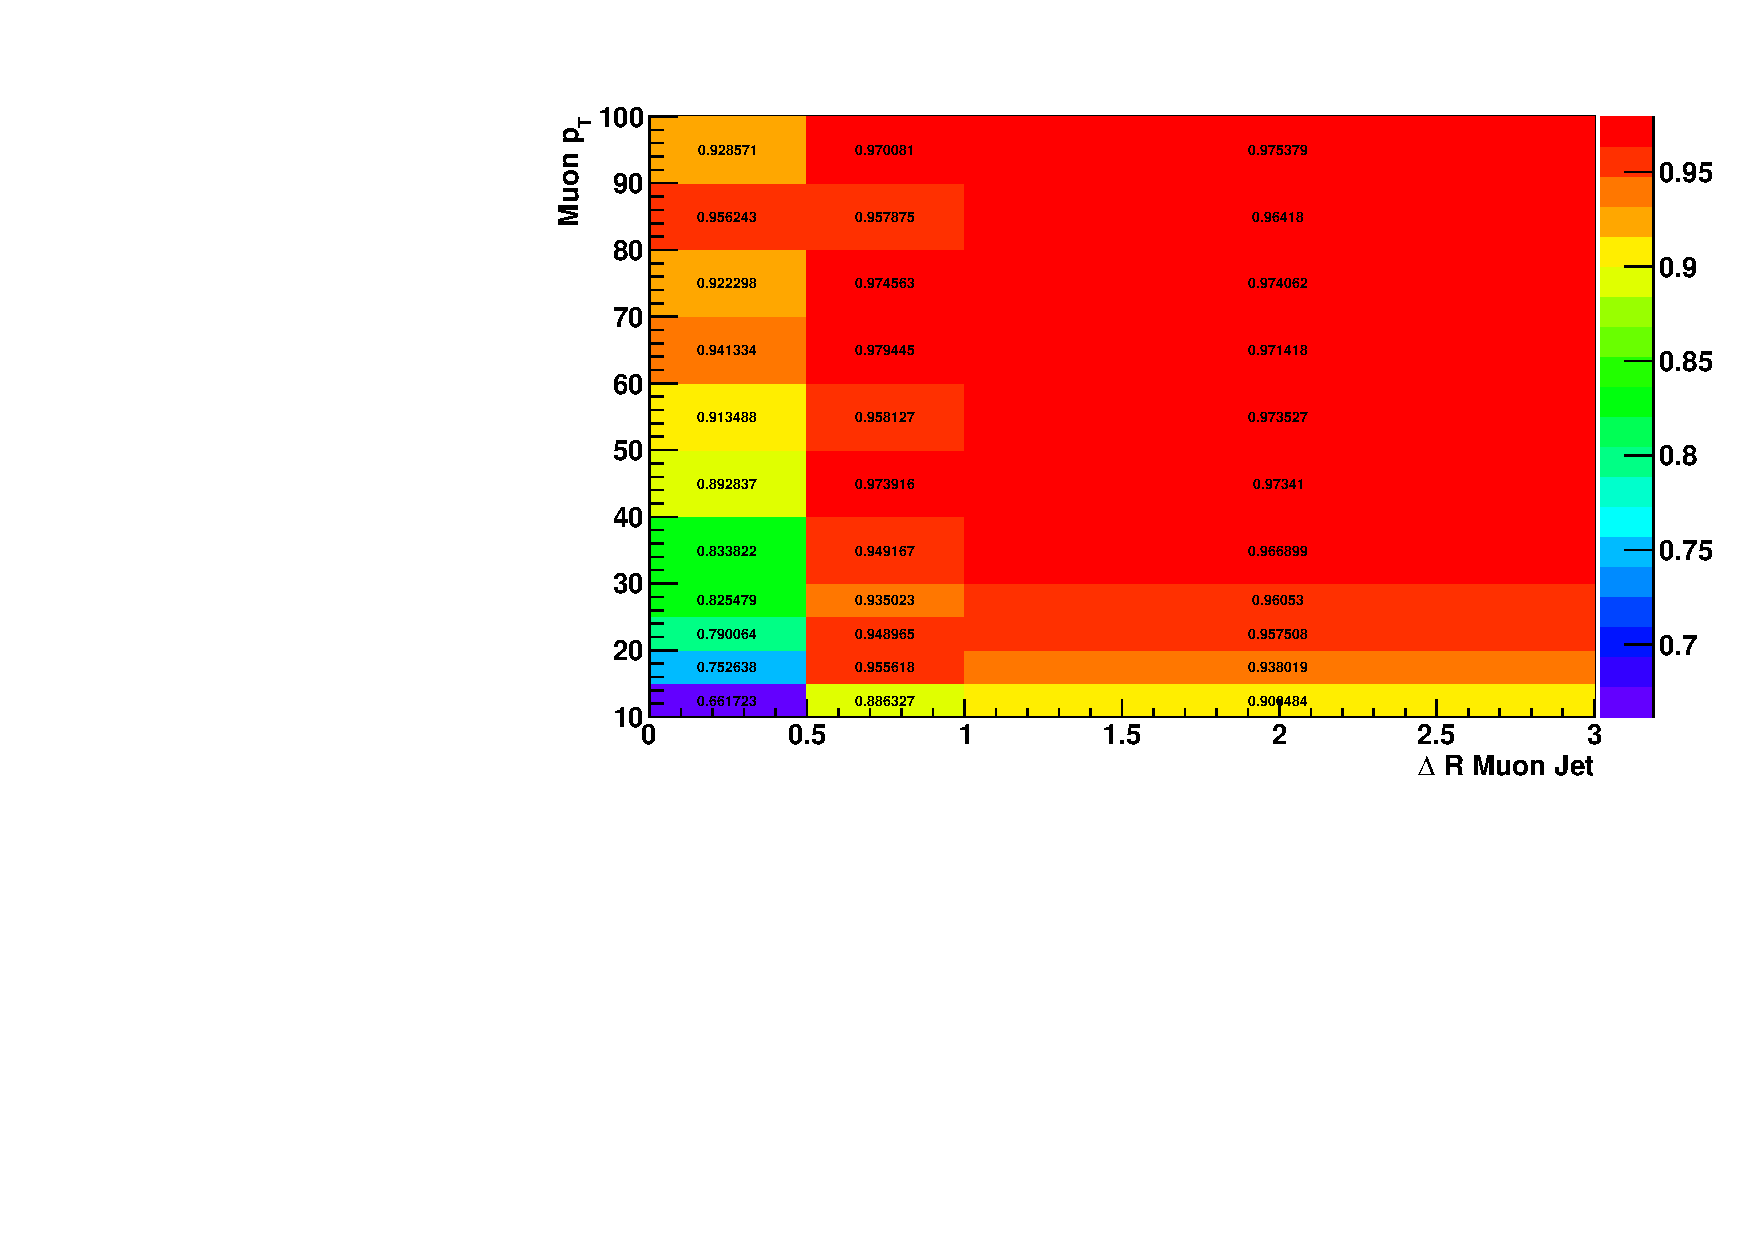
\includegraphics[width=.90\textwidth]{lostlepton/plots/Muon_Reco.pdf}\\
%\includegraphics[angle=0,width=0.5\textwidth]{wtop_lostlepton_figures/MHTMHT_r}&
%\includegraphics[angle=0,width=0.5\textwidth]{wtop_lostlepton_figures/HTHT_r}
%%(a)&(b)\\
\end{tabular}
\end{center}
\caption{These plots show the electron and $\mu$ reconstruction efficiencies obtained from MC.
}
\label{fig:reco_eff}
\end{figure}
%Fig. \ref{fig:not_reco} shows the distribution of not reconstructed  the right and not reconstructed muons on the left for \ttbar on top and for \wpj on the bottom separately. Good agreement between MC truth and MC prediction can be observed.
\clearpage

\subsection{Not isolated leptons}
\label{sec:isolation}
When a lepton is reconstructed it also has to fulfill the isolation criteria to be identified as a prompt lepton.
The applied isolation criteria are discussed in Sec.~\ref{sec:event_selection}.\\
Leptons show a higher isolation dependency on their \pt and angular distance relative to the closest jet.
Leading to the chosen efficiency parameterization in $\frac{p_{t,lep}}{p_{t,jet}}$ and $\Delta R$ to the closest jet. Especially for $\Delta R$ below 0.5 rad and low $\pt$ the efficiencies decrease strongly. To achieve as much accuracy as possible the $\Delta R$ binning has been optimized. However the statistics of the $Z$-sample are very limited in very small $\Delta R$. Fig.\ref{fig:iso_eff} shows the isolation efficiencies for electrons and $\mu$.
% iso eff
\begin{figure}[tbhn]
\begin{center}
\begin{tabular}{c}
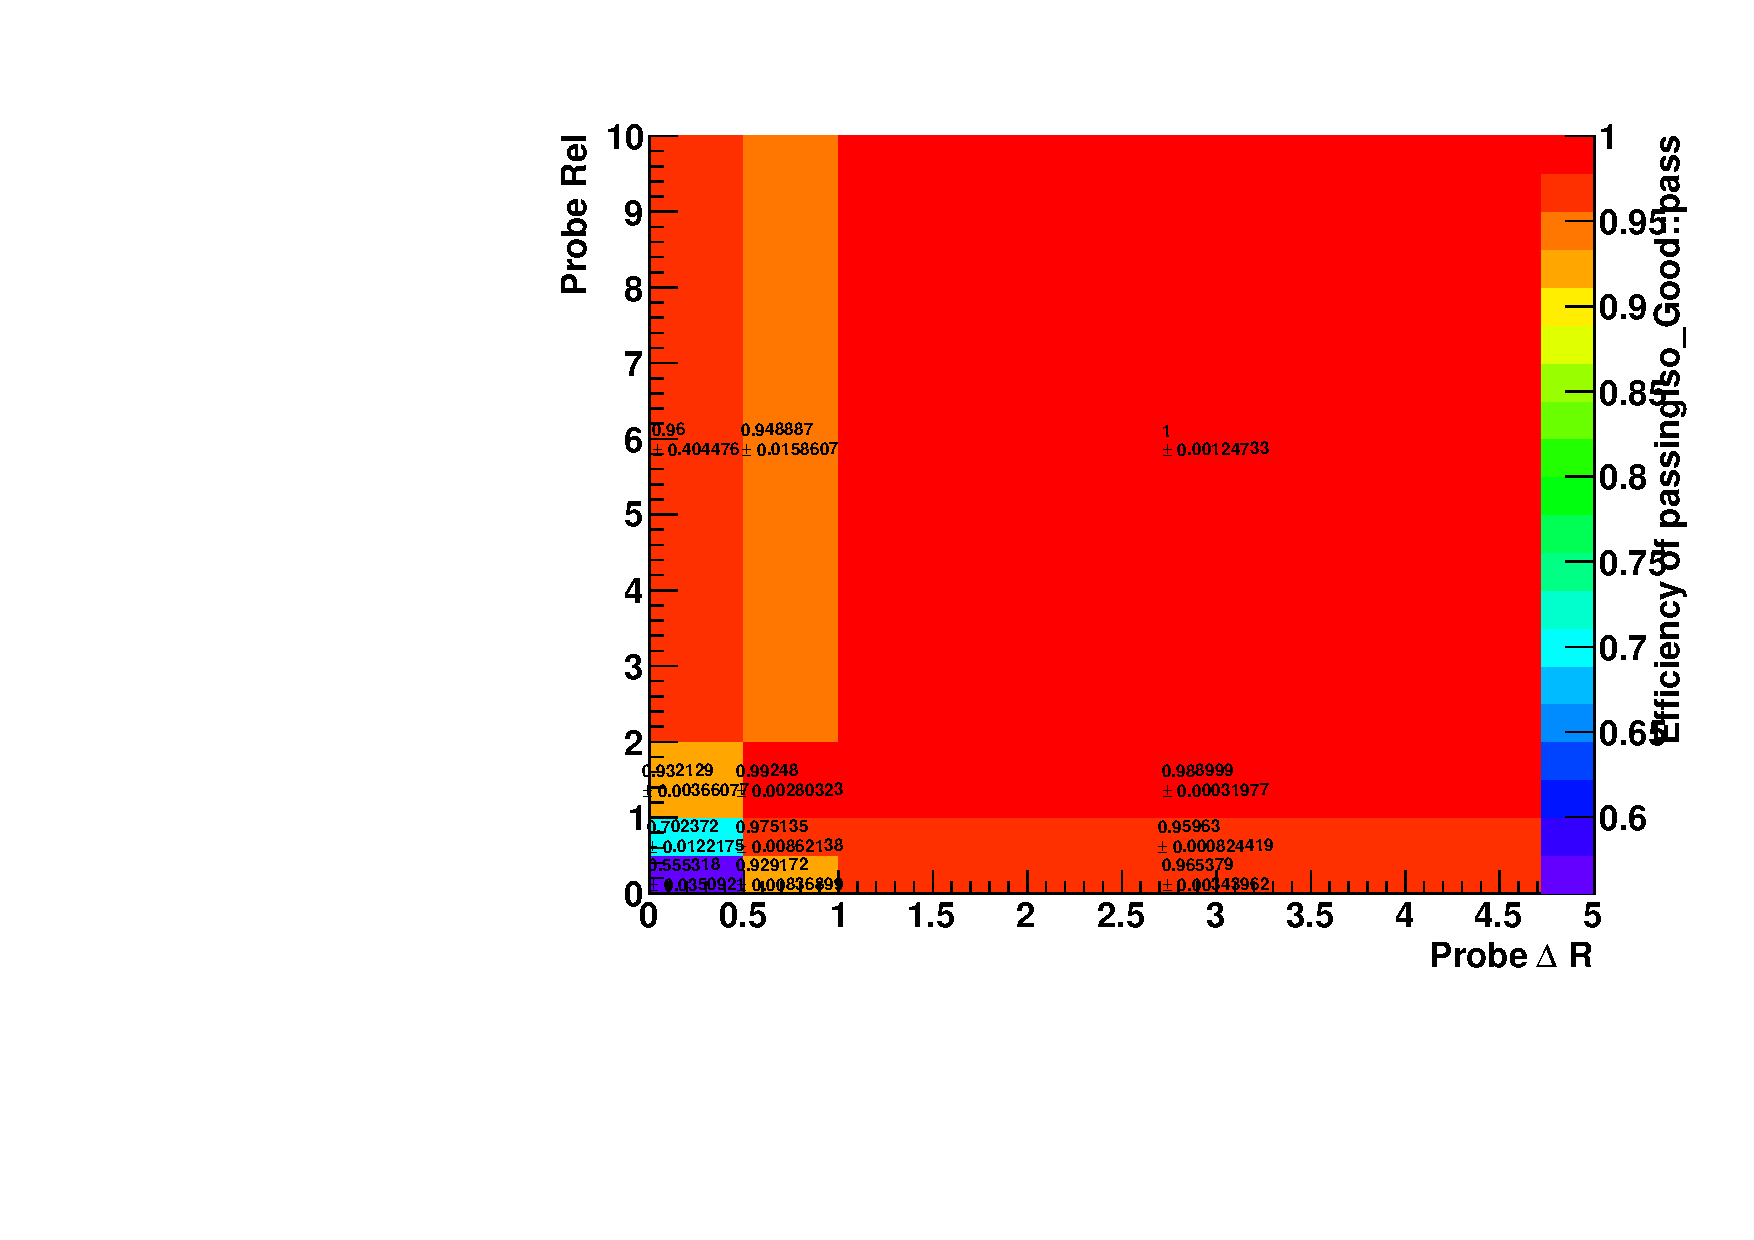
\includegraphics[width=.85\textwidth]{lostlepton/plots/Elec_Iso.pdf}\\
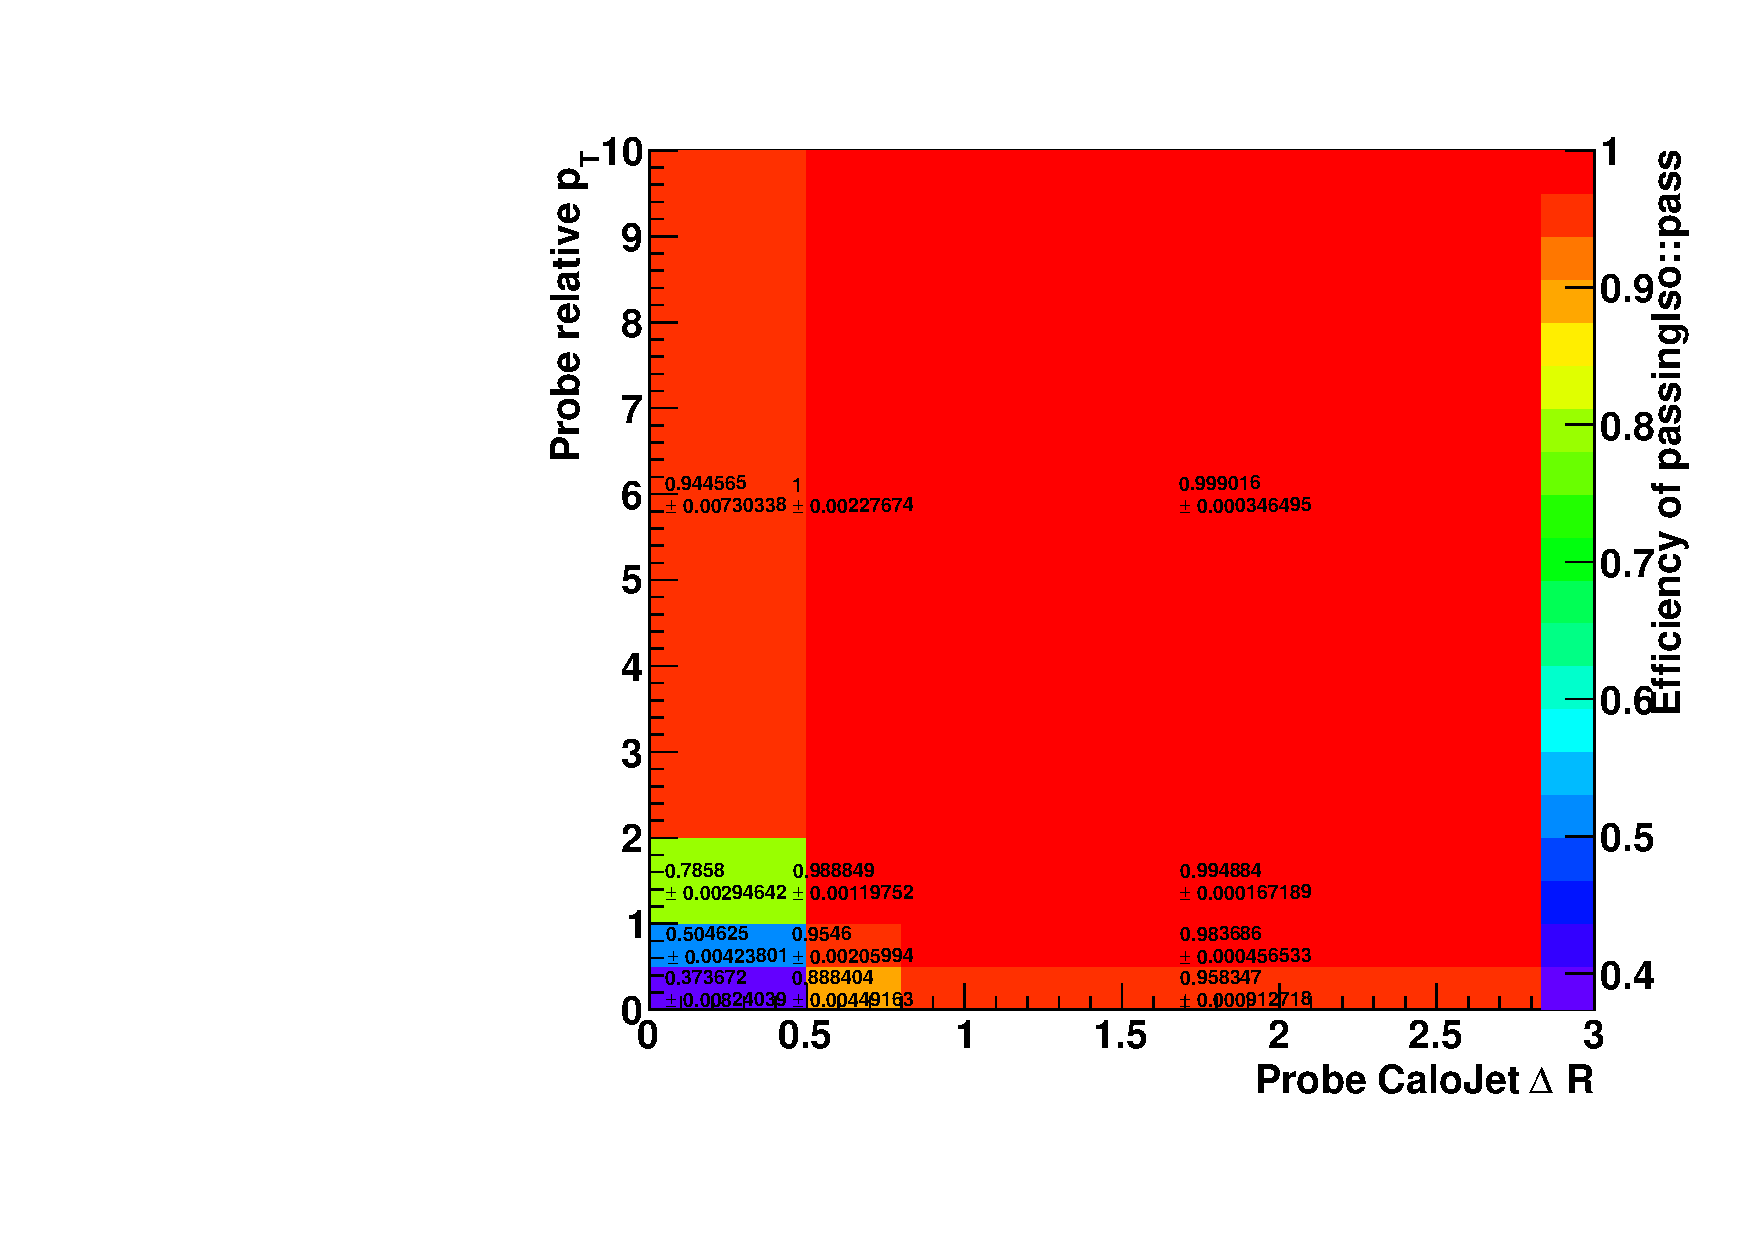
\includegraphics[width=.85\textwidth]{lostlepton/plots/Muon_Iso.pdf}\\
%\includegraphics[angle=0,width=0.5\textwidth]{wtop_lostlepton_figures/MHTMHT_r}&
%\includegraphics[angle=0,width=0.5\textwidth]{wtop_lostlepton_figures/HTHT_r}
%%(a)&(b)\\
\end{tabular}
\end{center}
\caption{These plots show the electron and $\mu$ isolation efficiencies calculated with a Tag\&Probe method.
}
\label{fig:iso_eff}
\end{figure}


\clearpage



\section{Closure tests and prediction on data}
\label{sec:closure_test}
Closure tests are a useful instrument of validating data driven methods on MC. For background estimations the prediction based on the MC control sample, labeled Data-driven Prediction from MC, is compared to the expected lost-leptons from MC, labeled MC expectation, in the signal region. Only statistical uncertainties are applied, since systematic uncertainties cancel within such a closure test.\\
One basic assumption of this method is that the topology of the CS and the signal sample do not differ considerable. The main search variables \HT and \MHT along with the number of primary vertices (see Sec.~\ref{sec:pileup})  are investigated to validate this assumption.\\ 
The closer test for the \HT and \MHT can be seen in Fig.~\ref{fig:closure}. Good agreement in shape can be observed. Tab.~\ref{tab:mc_closureA} contains the numbers of the Data-driven prediction on MC events compared to MC expectation for \ttbar and \wpj separately for the baseline selection. Also here good agreement can be observed. Despite a statistical significant discrepancy for the not reconstructed muons for \wpj and the not isolated muons for \ttbar, leading to an observed 4\% underestimation, called non-closure, for which a correction factor is applied on data, the closure tests show that the topology of the events including lost leptons and the CS events agree well and that the assumption of similar topologies is valid for the baseline selection. The observed underestimation is discussed in the following.\\
\begin{table}[htb]
\begin{center}
    \begin{tabular}{|l|ll|ll|}
        \hline
        ~    				& \ttbar expectation   & \ttbar predic.    & \wpj expectation       & \wpj predic.    \\ \hline %& combined truth &combined predic.\\ \hline
        $\mu$, out of acceptance  	& $51.1\pm 0.9$ & $47.7\pm 0.4$    & $79.6\pm 2.0$ & $80.3\pm 0.9$ \\ \hline %&  $130.7\pm 2.3$& $128.0\pm 1.0$\\ \hline
        $\mu$, not reconstructed  	& $16.6\pm 0.5$ & $17.4\pm 0.3$    & $18.3\pm 0.9$ & $15.7\pm 0.3$ \\ \hline  %&  $35.0\pm 1.1$& $33.1\pm 0.4$\\ \hline
        $\mu$, not isolated 		& $34.6\pm 0.7$ & $27.1\pm 0.6$    & $25.9\pm 1.1$ & $25.9\pm 1.1$ \\ \hline \hline%&  $60.5\pm 1.3$& $53.0\pm 1.0$\\ \hline \hline
        $e$, out of acceptance		& $57.1\pm 0.9$ & $55.5\pm 0.5$    & $88.4\pm 2.1$ & $90.8\pm 1.1$ \\ \hline%&  $145.5\pm 2.3$& $146.3\pm 1.2$\\ \hline
       	$e$, not reconstructed 		& $35.4\pm 0.7$ & $35.3\pm 0.4$    & $50.1\pm 1.5$ & $46.1\pm 0.7$ \\ \hline%&  $85.4\pm 1.7$& $81.5\pm 0.8$\\ \hline
        $e$, not isolated		& $28.5\pm 0.6$ & $21.0\pm 0.4$    & $21.5\pm 1.0$ & $21.2\pm 0.6$ \\ \hline \hline %&  $50.0\pm 1.2$& $42.2\pm 0.8$\\ \hline \hline
	total				& $219.2\pm 1.8$ & $204.1\pm 2.3$  & $285.0\pm 3.7$ & $280.0\pm 4.0$ \\ %&  $504.2\pm 4.1$& $484.1\pm 4.6$\\
        \hline
    \end{tabular}
\caption{This table shows the prediction on MC vs the expected events from MC. The numbers are scaled to \lumi.\label{tab:mc_closureA}}
\end{center}
\end{table}
Fig.~\ref{fig:closure_sepTTbar} and Fig.~\ref{fig:closure_sepW} show the closure test for \HT and \MHT for \ttbar and \wpj separately. For \wpj both the \MHT and \HT distribution agree well in shape. For \ttbar the \HT distribution agrees also well but the \MHT distribution shows an increasing under-prediction. Further closer tests have been done for the \ttbar \MHT distribution separately for not isolated, not reconstructed or out of the detector acceptance leptons.\\ %For completeness the closure plots for \wpj are also attached in the appendix.\\ 
The observed increasing under-prediction arises from the contribution of not isolation leptons and is passed to the other contribution since they also depend on the muon isolation efficiency (see Sec.~\ref{sec:ll_prediction}.\\
This observation can be understood by considering the boost of the \ttbar system at larger \MHT. The increasing boost of the top quarks leads to a shrinking angular distance, $\Delta R$, between the $b$-jet and the $W$. The final decay products, the lepton and the $\nu$, are also boosted resulting in an increased \MHT and smaller angular distance $\Delta R$ between the lepton and the $b$-jet. The under-prediction arises now since the isolation efficiencies decrease strongly with $\Delta R$ approaching 0 and as stated in Sec.~\ref{sec:tag_probe} it is not possible to parametrize the binning of the efficiencies $\Delta R$ any smaller. This incapability of the method to account for this extreme boosted systems with this very small $\Delta R$ is unavoidably and results in the observed increasing non-closure with increasing \MHT.\\
For the \wpj sample a similar dependency is not expected because there is no correlation between \MHT and $\Delta R$.\\ 
This well understood systematic under-prediction justifies the correction factor of 4\% applied on data together with an additional uncertainty, introduced in Sec.~\ref{sec:uncertainties}, covering this dependency and other possible remaining differences in the closure, eg. the observed non-closure for the not reconstructed muons in the \wpj sample.\\
Fig.~\ref{fig:reco_acc_combined} shows the \ttbar and \wpj combined closure test for the out of acceptance and not reconstructed fraction for electrons and muons separately. Together with the numbers from Tab.~\ref{tab:mc_closureA} one can observe good agreement for the not reconstructed and out of acceptance contribution.\\
Since it is not possible to separate the lost-lepton background from the other backgrounds, equivalent closure tests on data can not be done. Instead the $\mu$ CS from MC and data, and the prediction on data and MC are compared, as can be seen in Fig.~\ref{fig:LostLepton_MuCS_data_MC} and Fig.~\ref{fig:predicDataMC}. \\
For both distributions a good agreement in shape can be observed. However both the control sample and the prediction show a significant difference (see Tab.~\ref{tab:LostLeptonCompare}) but the idea of data-driven background estimation is to be independent from MC. The observed differences are expected to origin from deficiencies in the MC simulation.\\ 
Tab.~\ref{tab:LostLeptonCompare} contains the event yields on data, the Data-driven Prediction from MC and the MC Expectation. The prediction for the different search regions on data (defined in Sec.~\ref{sec:event_selection}) including all systematics uncertainties (discussed in Sec.~\ref{sec:uncertainties}) are shown in Tab.~\ref{tab:LostLeptonResult1}.
\begin{table}[hbt]
\selectfont
\begin{centering}
\caption[]{This table contains the final event yield for the lost-lepton background for the baseline selection on data and Data-driven Prediction from MC together with MC Expectation\footnote{The observed MC events are scaled to the full luminosity of \lumi.}. All uncertainties are included for the prediction on data. For the MC Expectation jet energy scale and luminosity uncertainties are applied and for the prediction on MC only statistical uncertainties are included.\label{tab:LostLeptonCompare} } 

\hspace*{-4ex}
\begin{tabular}{|c|c|c|c|}
\hline
\			& Pred. & Stat. Error	& Tot. Sys.		\\
\hline 
prediction on data	&453.5	&$\pm 26.3$	&$^{+52.5}_{-53.4}$	\\
MC Expectation	    	&545.8  &$\pm 4.5$	&$^{+50.4}_{-51.1}$	\\
Data-driven Prediction from MC	&524.1	&$\pm 5.0$	&	\\ \hline

\end{tabular}
\par\end{centering}
\end{table}

% 
\begin{figure}[tbhn]
\begin{center}
\begin{tabular}{cc}
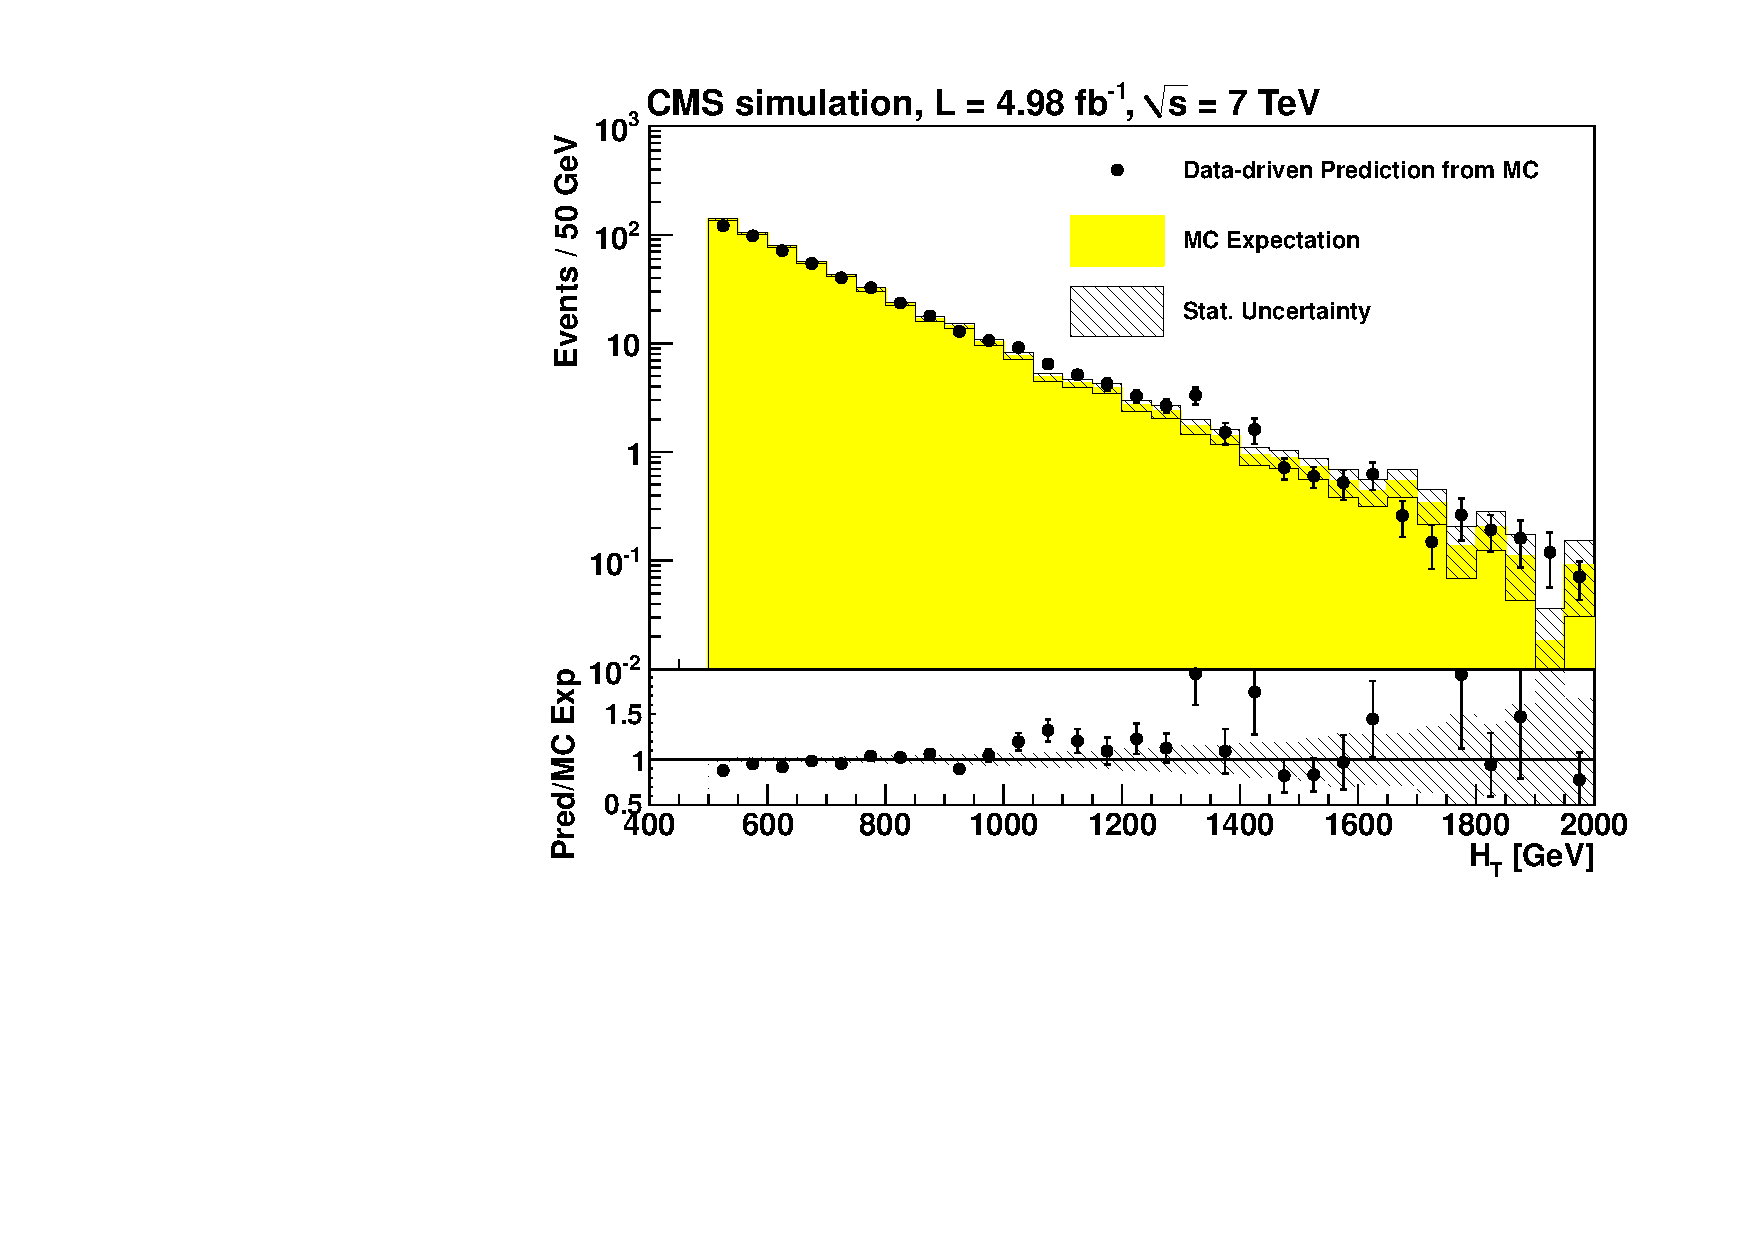
\includegraphics[width=0.90\textwidth]{lostlepton/plots/ANplots/Closure_HT.pdf}\\
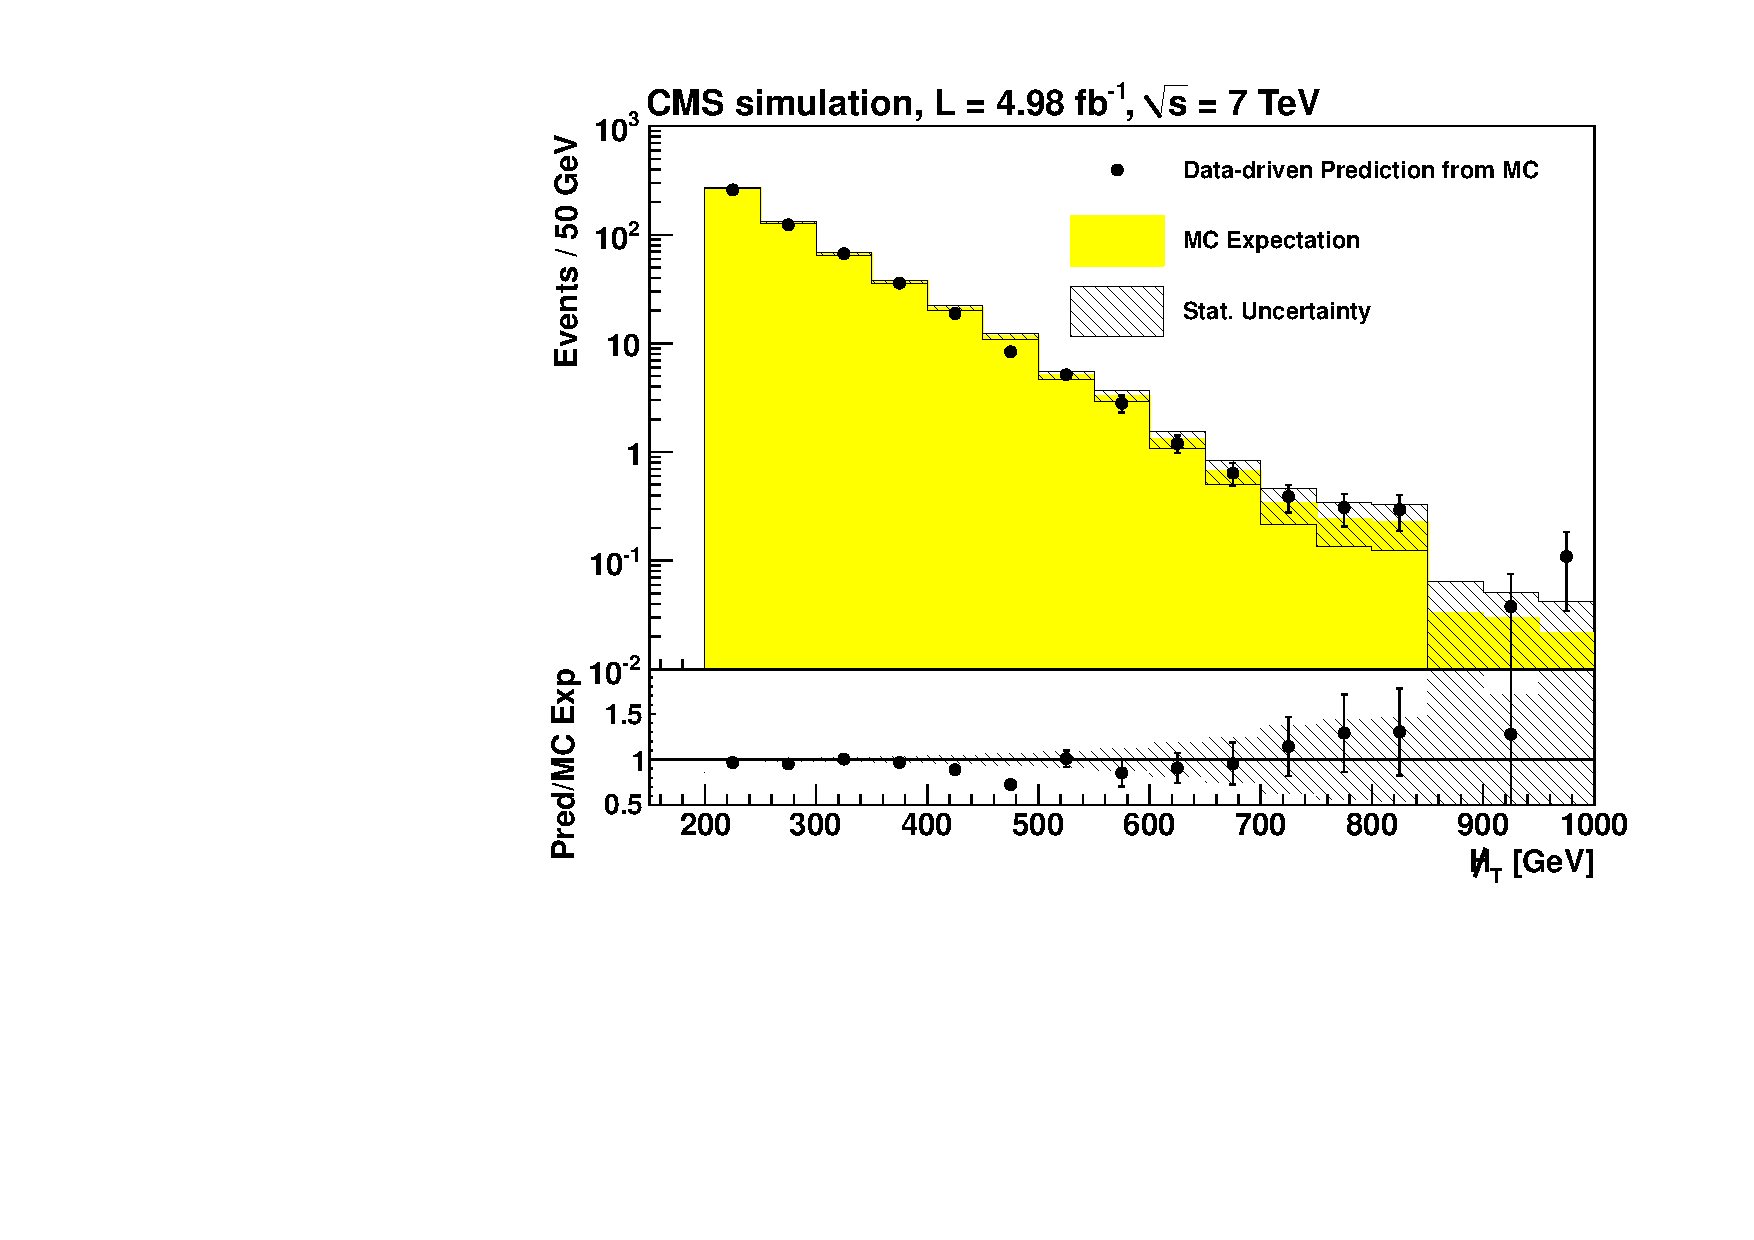
\includegraphics[width=0.90\textwidth]{lostlepton/plots/ANplots/Closure_MHT.pdf}

%\includegraphics[angle=0,width=0.5\textwidth]{wtop_lostlepton_figures/MHTMHT_r}&
%\includegraphics[angle=0,width=0.5\textwidth]{wtop_lostlepton_figures/HTHT_r}
%%(a)&(b)\\
\end{tabular}
\end{center}
\caption{These plots show the closure test for the \HT and \MHT baseline selection for the total lost-lepton background. The estimated lost-leptons are called Data-driven Prediction from MC, which refers to \ttbar and \wpj events combined and the observed lost-leptons are referred to as MC expectation.}
\label{fig:closure}
\end{figure}
%The method is tested in different distributions, the important search variable \MHT and \HT of course but also for jet-multiplicity and number of primary vertices(see sec. \ref{sec:pileup}). For validation the numbers in table \ref{tab:mc_closure} and the separated plots are used.
%The closure test has been done for \ttbar and \wpj separately and also for all the different contribution to the total lost lepton background. in the following each sample is discussed separately and the closure is interpreted.





% prediction on data vs mc
\begin{figure}[tbhn]
\begin{center}
\begin{tabular}{cc}
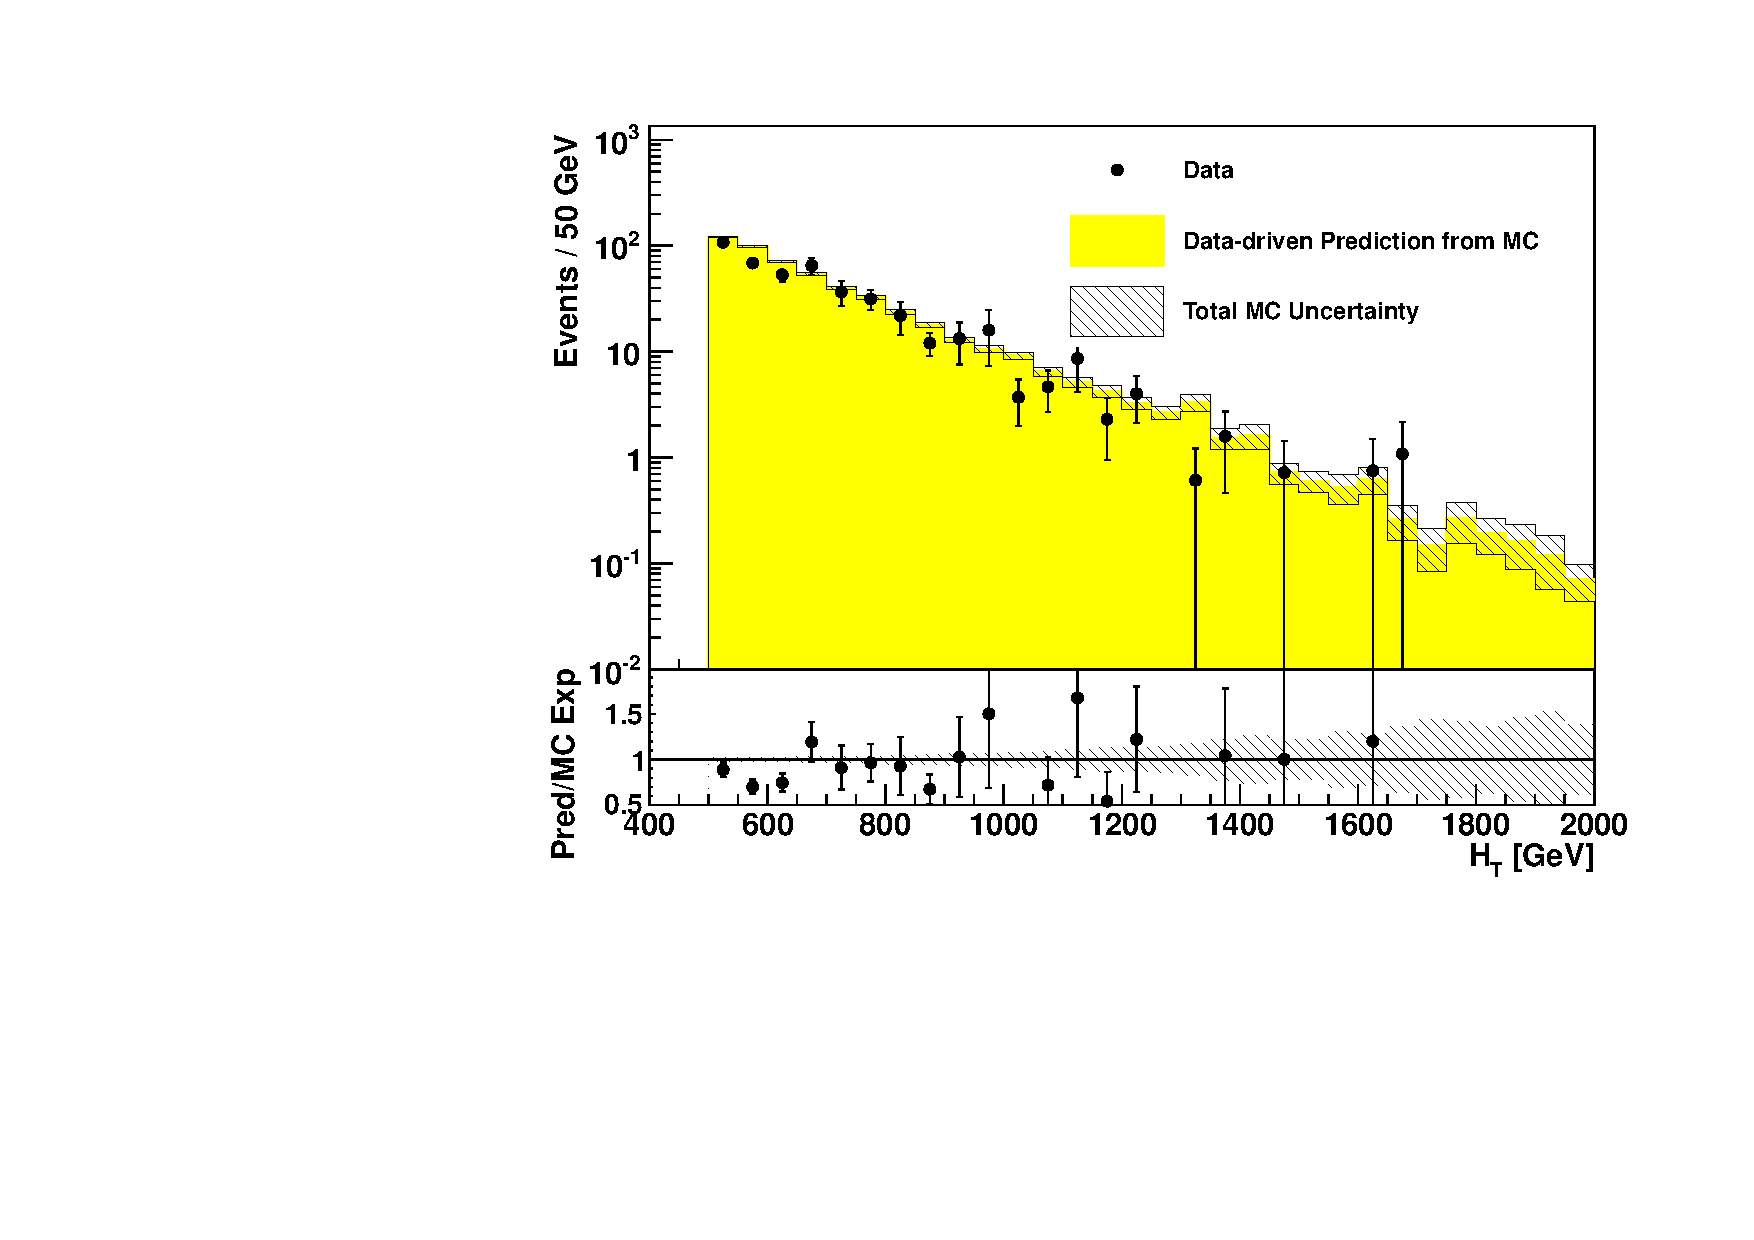
\includegraphics[width=0.90\textwidth]{lostlepton/plots/closure/DataVsMCPredictionHT.pdf}\\
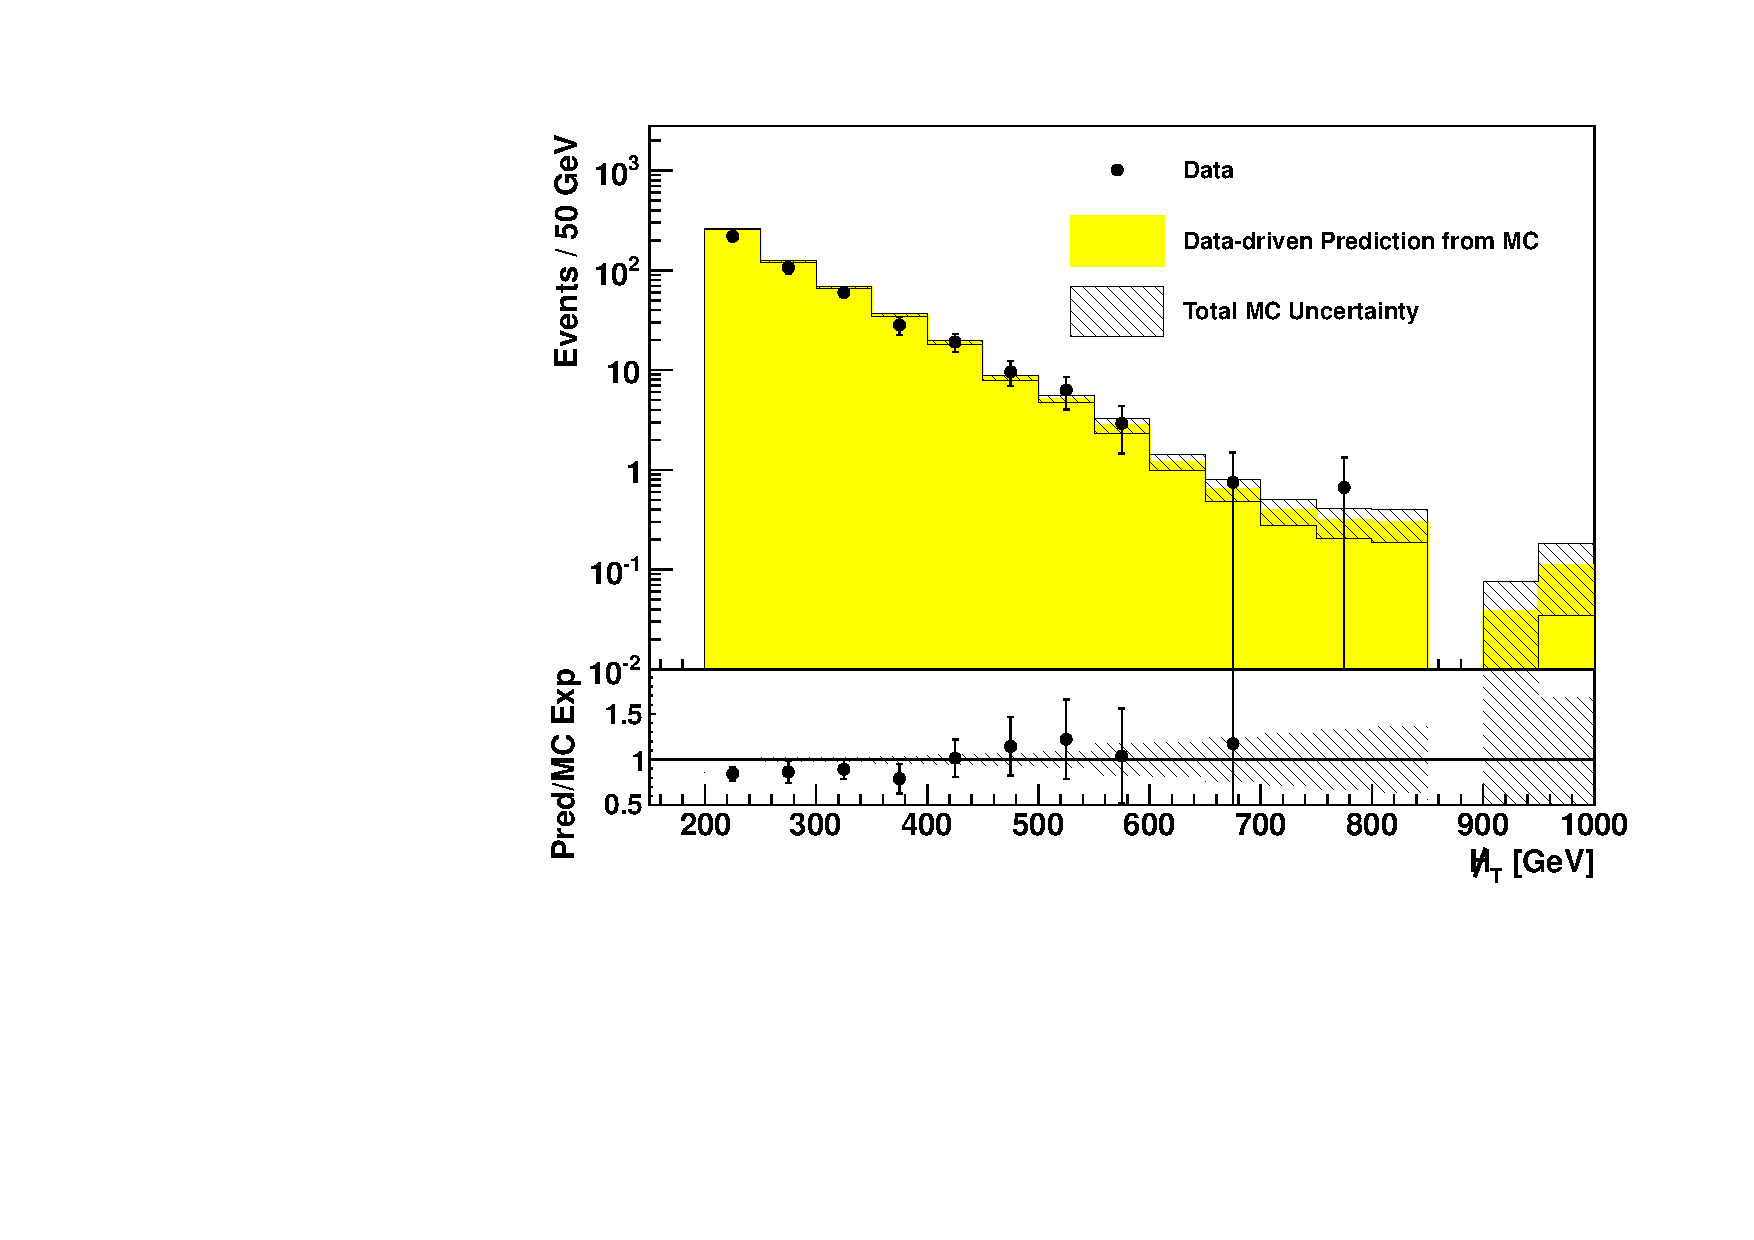
\includegraphics[width=0.90\textwidth]{lostlepton/plots/closure/DataVsMCPredictionMHT.pdf}

%\includegraphics[angle=0,width=0.5\textwidth]{wtop_lostlepton_figures/MHTMHT_r}&
%\includegraphics[angle=0,width=0.5\textwidth]{wtop_lostlepton_figures/HTHT_r}
%%(a)&(b)\\
\end{tabular}
\end{center}
\caption{Comparison of the prediction on data vs. the prediction on MC (\ttbar and \wpj combined) for the \HT (on the right) and the \MHT (on the left) distribution. For the data prediction all uncertainties are shown while for the MC prediction only statistical uncertainties are shown. The shapes agree well within the uncertainties.}
\label{fig:predicDataMC}
\end{figure}


%\subsection{\wpj closure test}
%\label{wpj_closure}
%The overall closure for the \wpj sample shows a really good agreement in numbers (see tab. \ref{tab:mc_closure}) and shape (see fig. \ref{fig:wpj_closure}).

% leading jet pt and number of jets
%\begin{figure}[tbhn]
%\begin{center}
%\begin{tabular}{cc}
%\includegraphics[width=0.50\textwidth]{lostlepton/plots/closure/ttbar/Jet1PtClosure.pdf}
%\includegraphics[width=0.50\textwidth]{lostlepton/plots/closure/w/Jet1PtClosure.pdf}
%\includegraphics[angle=0,width=0.5\textwidth]{wtop_lostlepton_figures/MHTMHT_r}&
%\includegraphics[angle=0,width=0.5\textwidth]{wtop_lostlepton_figures/HTHT_r}
%%(a)&(b)\\
%\end{tabular}
%\end{center}
%\caption{This plots show a closure test for the \pt of the leading jet for \ttbar and \wpj. Good agreement of the shape as well as the ratio can be seen.
%}
%\label{fig:jet_closure}
%\end{figure}

% leading jet pt and number of jets
\begin{figure}[tbhn]
\begin{center}
\begin{tabular}{cc}
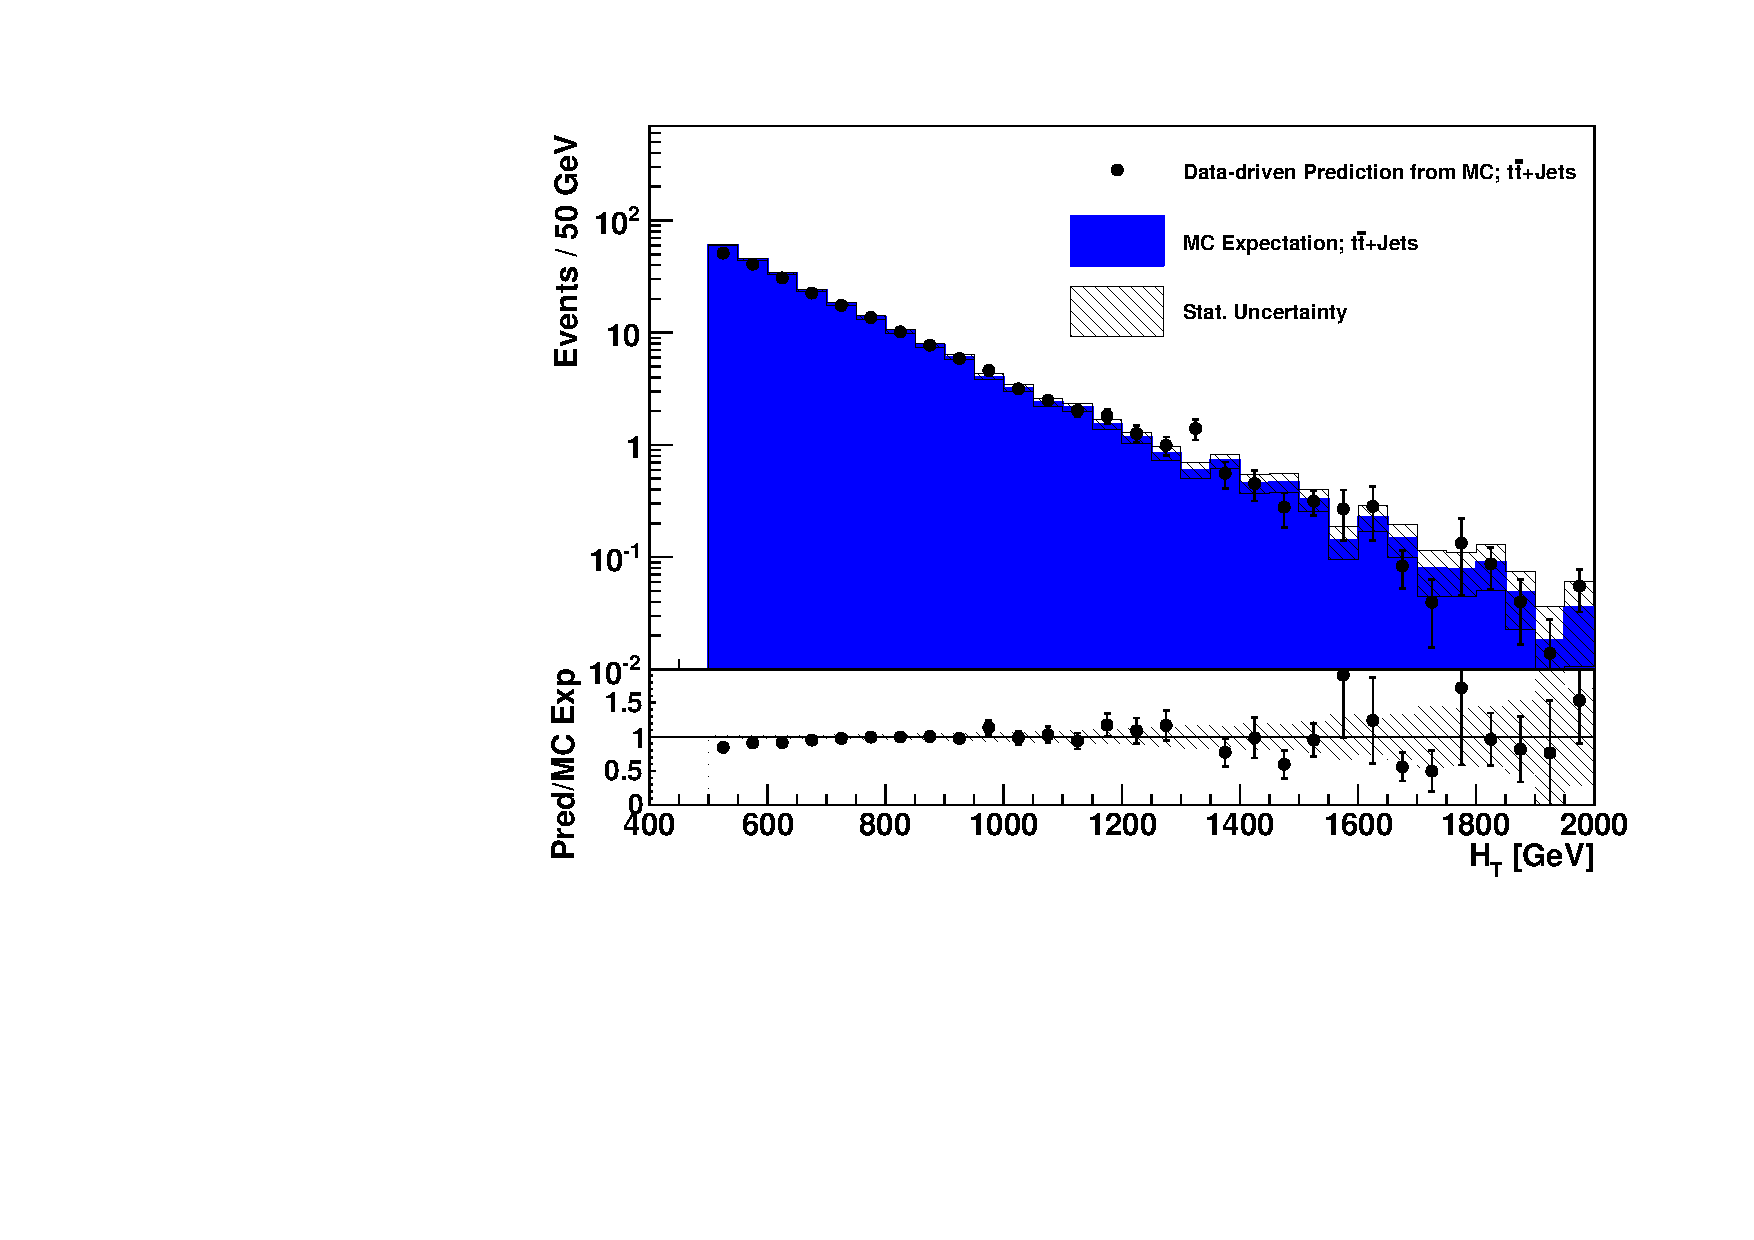
\includegraphics[width=0.90\textwidth]{lostlepton/plots/closure/HTttbar.pdf}\\
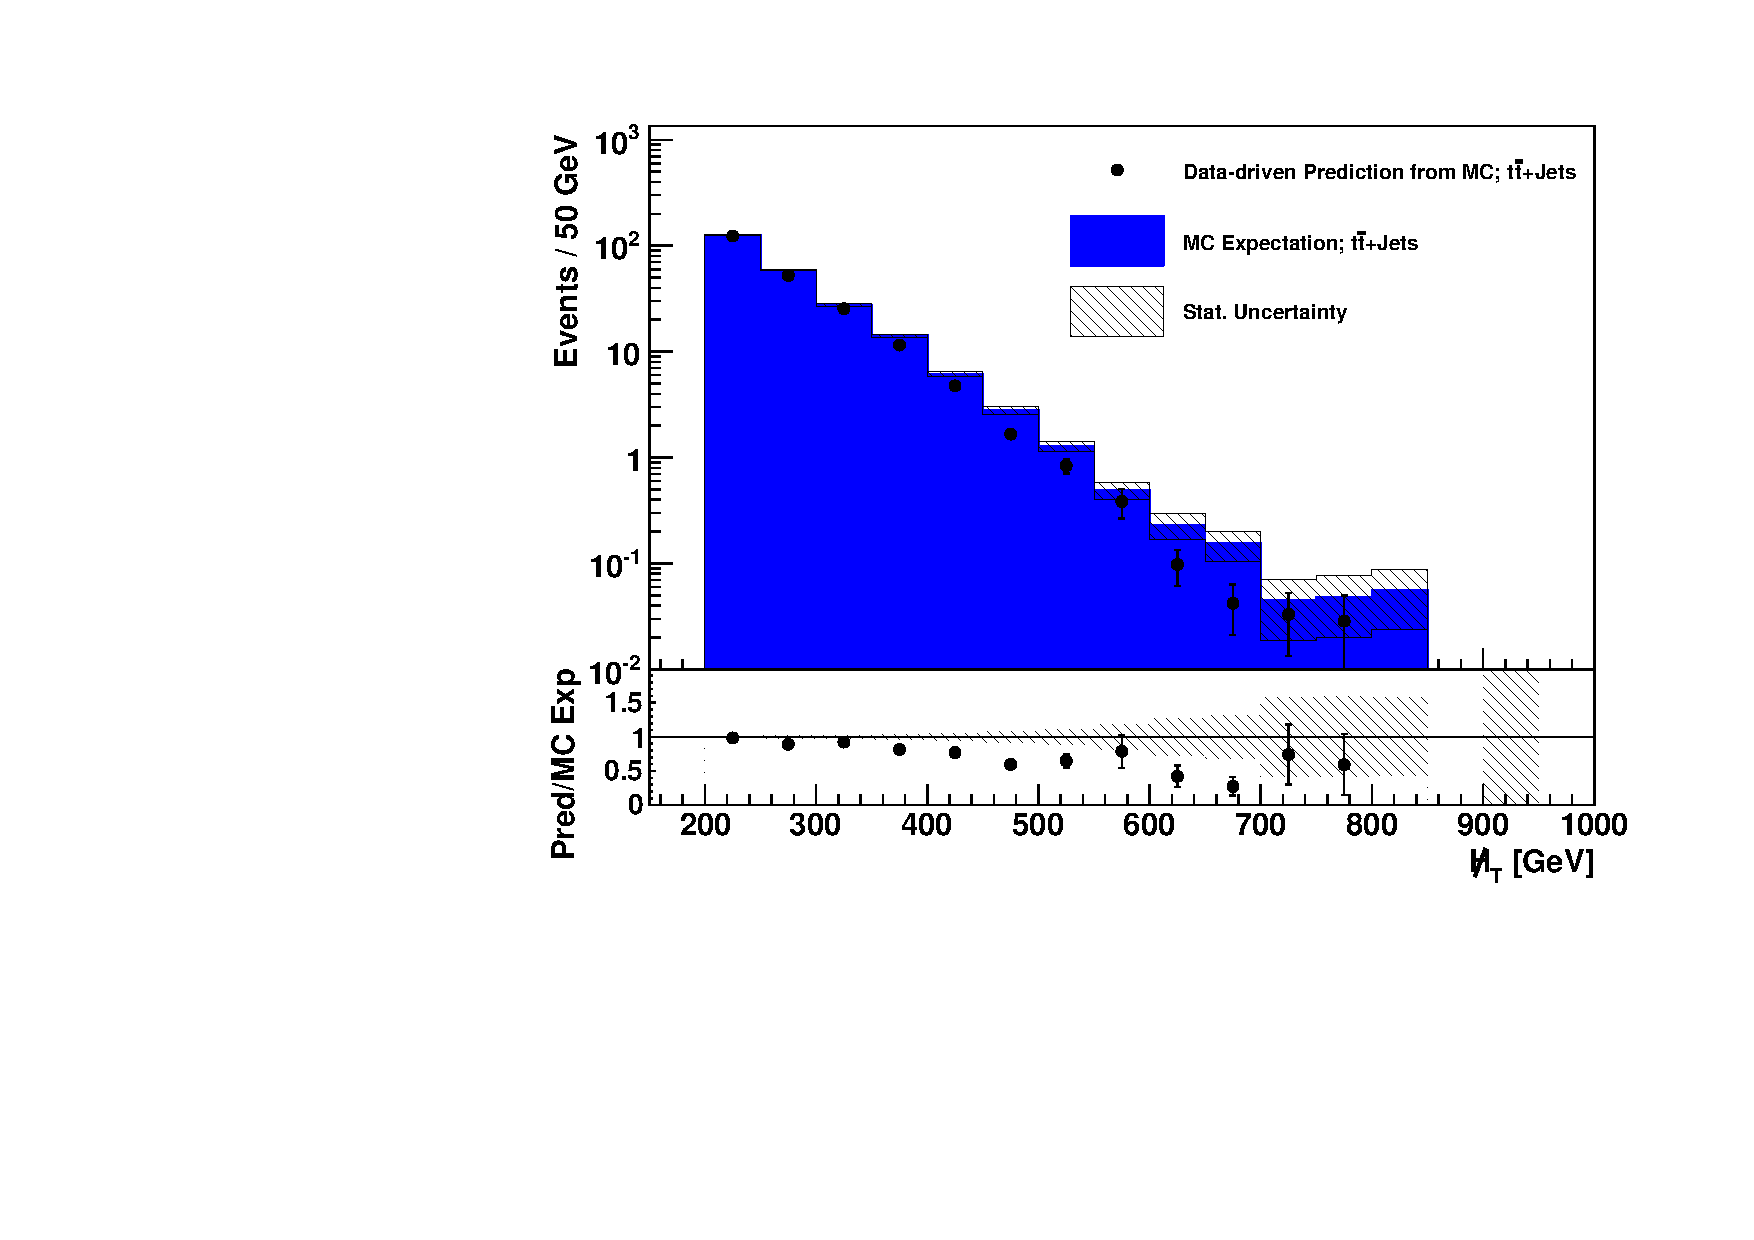
\includegraphics[width=0.90\textwidth]{lostlepton/plots/closure/MHTttbar.pdf}

%\includegraphics[angle=0,width=0.5\textwidth]{wtop_lostlepton_figures/MHTMHT_r}&
%\includegraphics[angle=0,width=0.5\textwidth]{wtop_lostlepton_figures/HTHT_r}
%%(a)&(b)\\
\end{tabular}
\end{center}
\caption{This plots show the closure test of the Data-driven Prediction from MC and the MC expectation for the \HT and \MHT distribution for \ttbar simulated events. Good agreement of the shape as well as the ratio can be seen. Only the \MHT distribution shows a significant discrepancy.
}
\label{fig:closure_sepTTbar}
\end{figure}
\begin{figure}[tbhn]
\begin{center}
\begin{tabular}{cc}

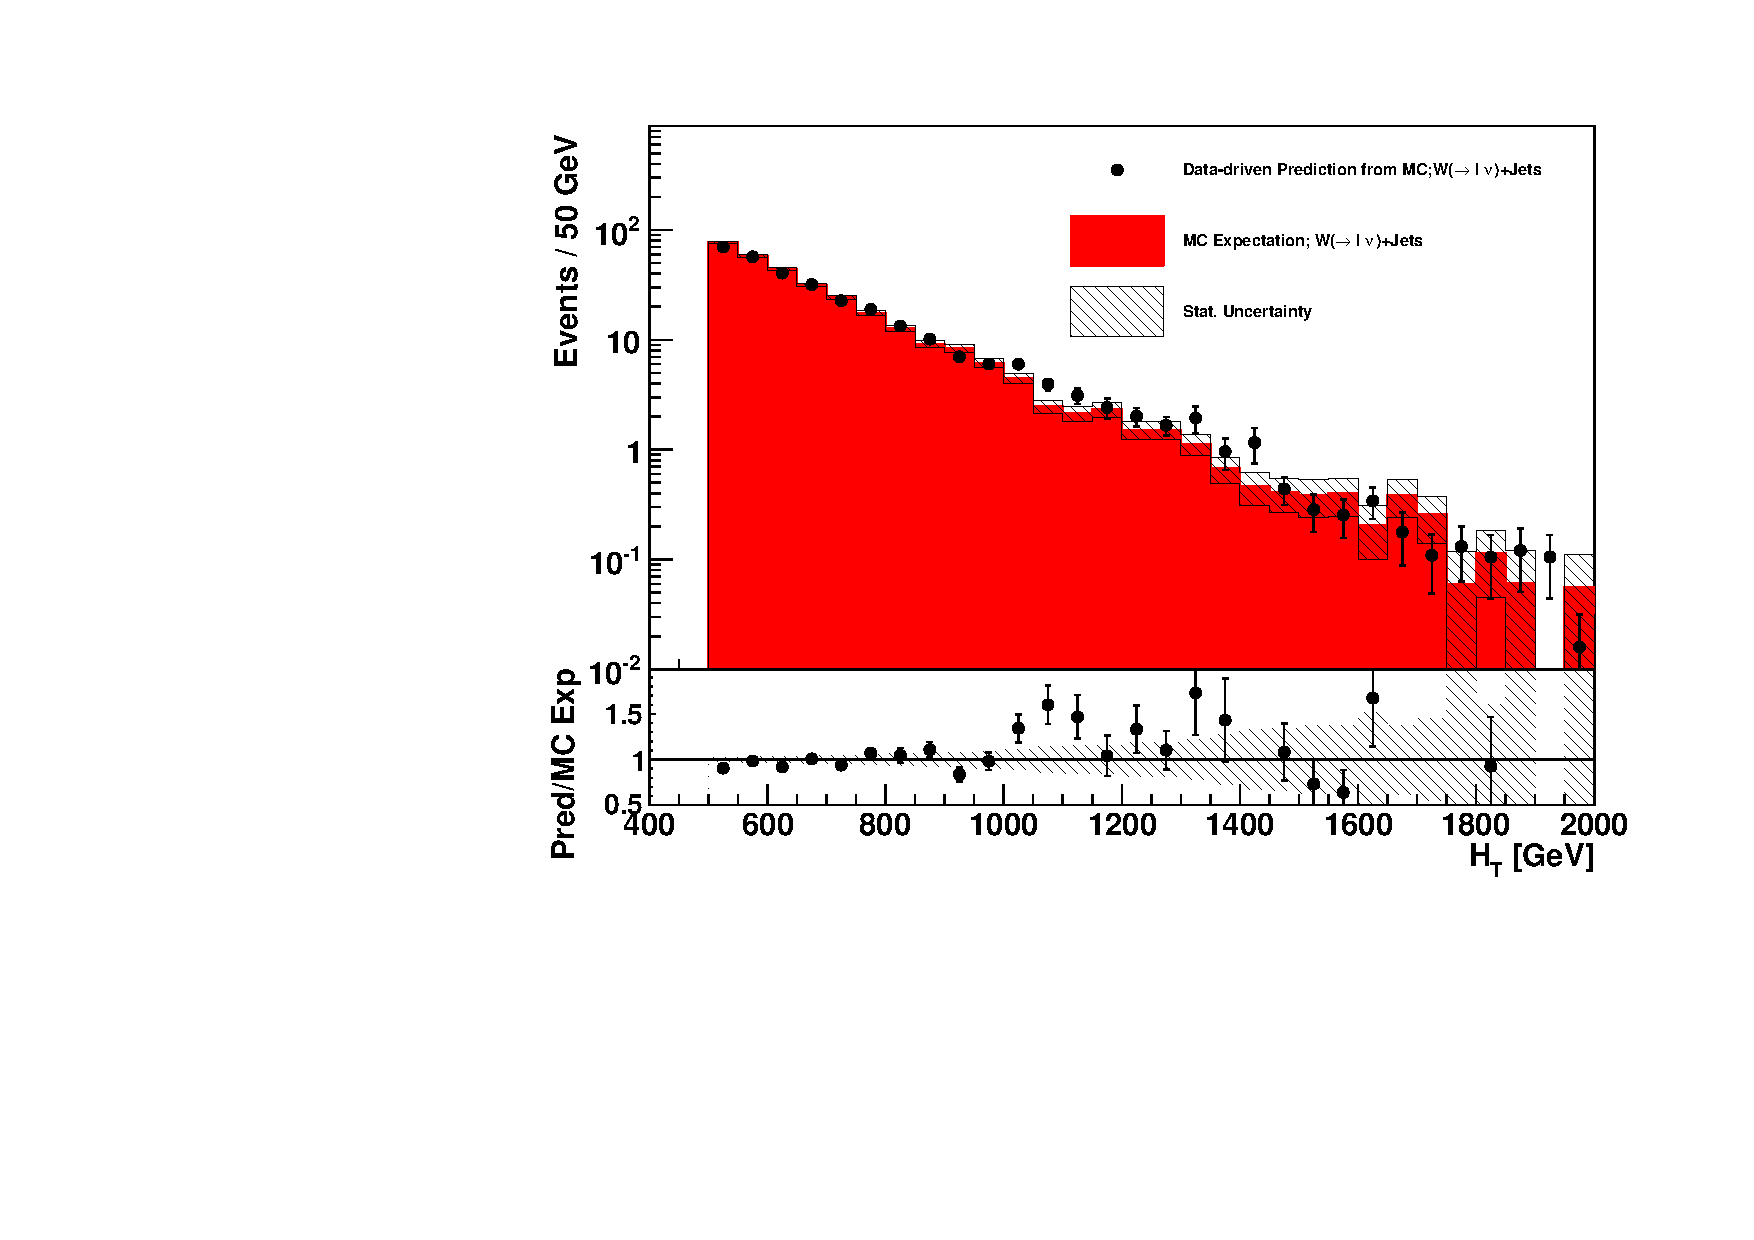
\includegraphics[width=0.90\textwidth]{lostlepton/plots/closure/HTw.pdf}\\
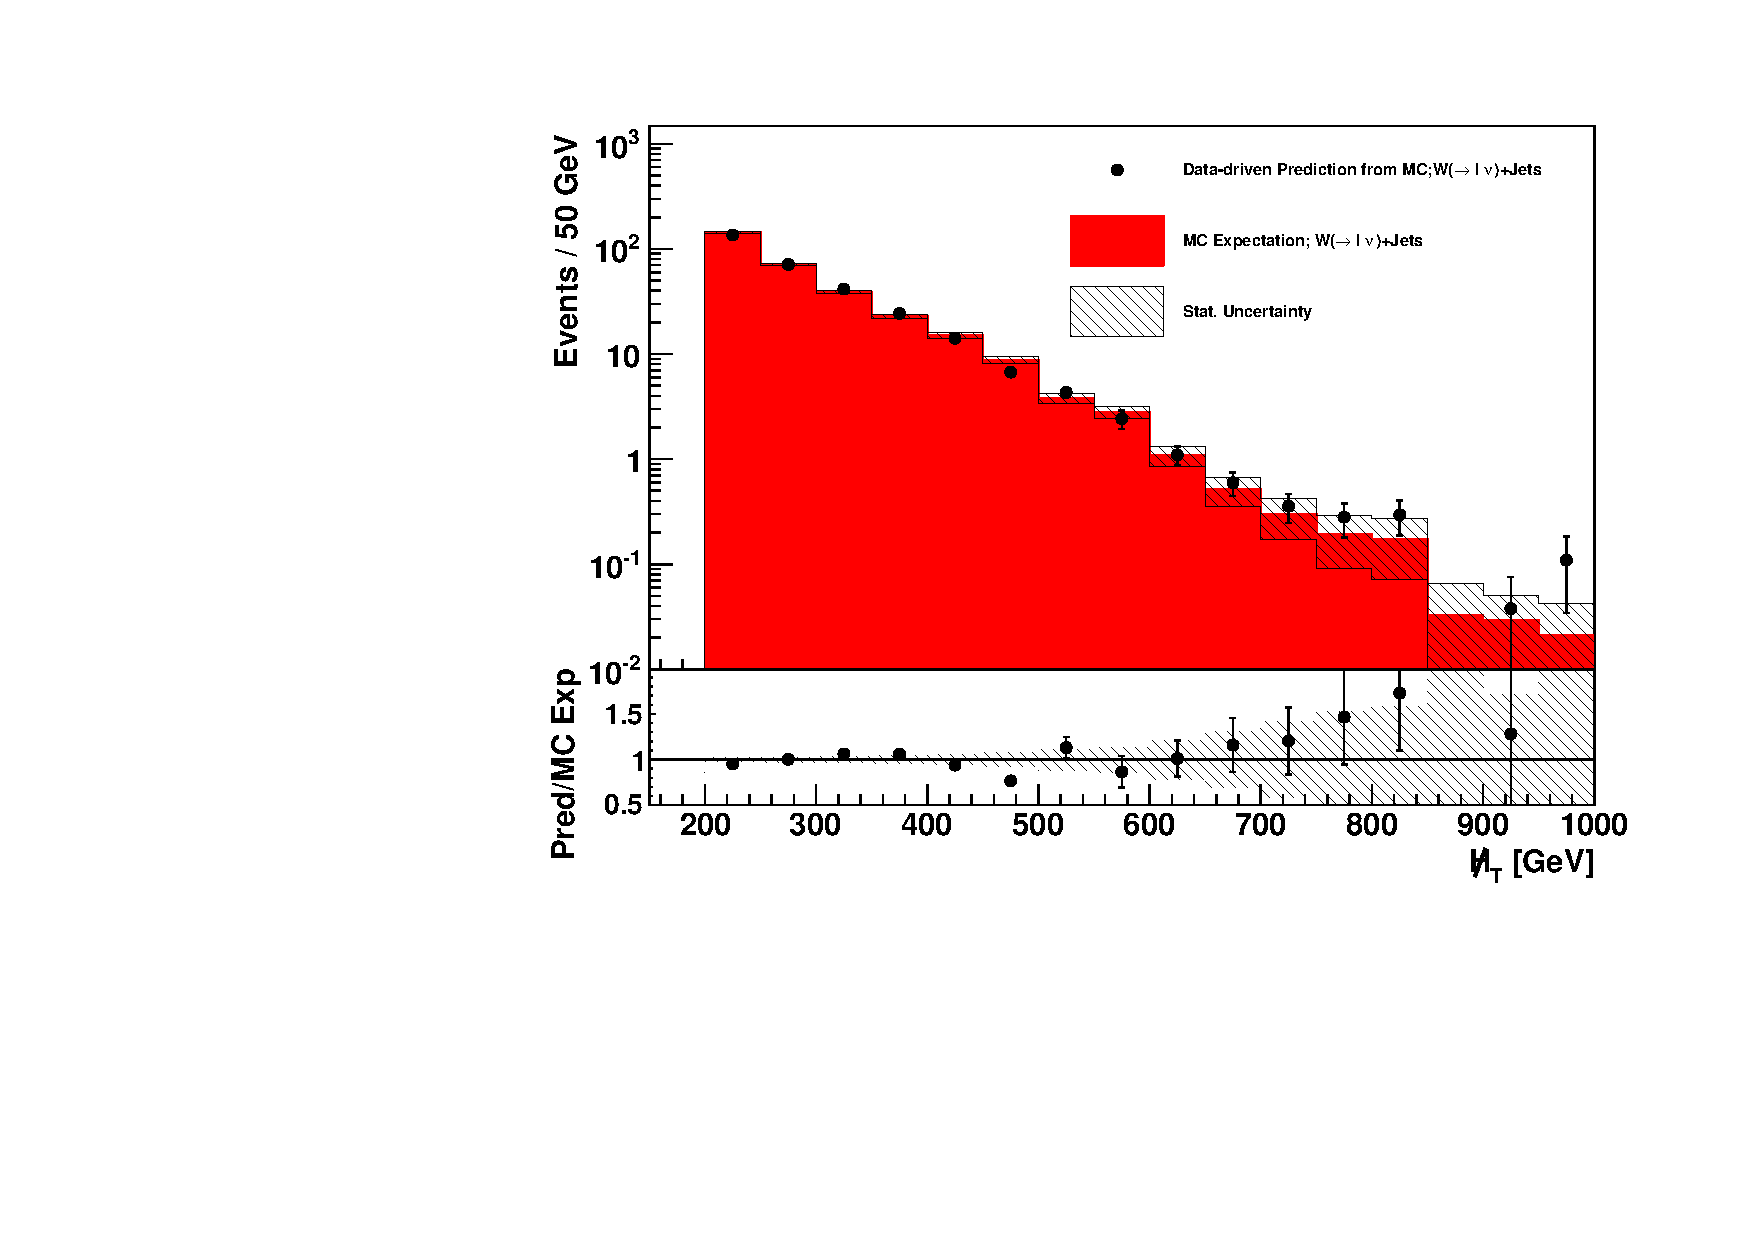
\includegraphics[width=0.90\textwidth]{lostlepton/plots/closure/MHTw.pdf}
%\includegraphics[angle=0,width=0.5\textwidth]{wtop_lostlepton_figures/MHTMHT_r}&
%\includegraphics[angle=0,width=0.5\textwidth]{wtop_lostlepton_figures/HTHT_r}
%%(a)&(b)\\
\end{tabular}
\end{center}
\caption{This plots show the closure test of the Data-driven Prediction from MC and the MC expectation for the \HT and \MHT distribution for \wpj simulated events. Good agreement of the shape as well as the ratio can be seen.}
\label{fig:closure_sepW}
\end{figure}





% ttbar MHT closure iso reco acc
\begin{figure}[tbhn]
\begin{center}
\begin{tabular}{cc}
\includegraphics[width=0.50\textwidth]{lostlepton/plots/closure/MHTttbarIsoMu.pdf} 
\includegraphics[width=0.50\textwidth]{lostlepton/plots/closure/MHTttbarIsoE.pdf} \\
\includegraphics[width=0.50\textwidth]{lostlepton/plots/closure/MHTttbarRecoMu.pdf}
\includegraphics[width=0.50\textwidth]{lostlepton/plots/closure/MHTttbarRecoE.pdf}\\
\includegraphics[width=0.50\textwidth]{lostlepton/plots/closure/MHTttbarAccMu.pdf}
\includegraphics[width=0.50\textwidth]{lostlepton/plots/closure/MHTttbarAccE.pdf}\\
%\includegraphics[angle=0,width=0.5\textwidth]{wtop_lostlepton_figures/MHTMHT_r}&
%\includegraphics[angle=0,width=0.5\textwidth]{wtop_lostlepton_figures/HTHT_r}
%%(a)&(b)\\
\end{tabular}
\end{center}
\caption{This plots show the closure tests for \ttbar events separated for the not isolated (top), not reconstructed (middle) and out of acceptance fraction (bottom). Good agreement for the shape can be observed. However, an increasing under-prediction can also be seen. The legend description can be found in the caption of Fig.~\ref{fig:closure_sepTTbar}.
}
\label{fig:closure_ttbar_sep_MHT}
\end{figure}


% leading jet pt and number of jets
\begin{figure}[tbhn]
\begin{center}
\begin{tabular}{cc}
\includegraphics[width=0.50\textwidth]{lostlepton/plots/closure/MCClosureRecoMuMHT.pdf}
\includegraphics[width=0.50\textwidth]{lostlepton/plots/closure/MCClosureRecoEMHT.pdf}\\
\includegraphics[width=0.50\textwidth]{lostlepton/plots/closure/MCClosureAccMuMHT.pdf}
\includegraphics[width=0.50\textwidth]{lostlepton/plots/closure/MCClosureAccEMHT.pdf}\\
%\includegraphics[angle=0,width=0.5\textwidth]{wtop_lostlepton_figures/MHTMHT_r}&
%\includegraphics[angle=0,width=0.5\textwidth]{wtop_lostlepton_figures/HTHT_r}
%%(a)&(b)\\
\end{tabular}
\end{center}
\caption{The upper two plots show the closure test for the not reconstructed muon on the left and for electrons on the right for \ttbar and \wpj combined. On the bottom the same is shown for the out of acceptance background contribution. The legend description can be found in the caption of Fig.~\ref{fig:closure_sepTTbar}.
}
\label{fig:reco_acc_combined}
\end{figure}

\clearpage


 







% numbers of CS on data and MC



\begin{sidewaystable}[hbt]
%\fontsize{8 pt}{1.0 em}
\selectfont
\begin{centering}
\caption[]{Final event yield for the lost-lepton background for the exclusive search
regions. The numbers are for the full luminosity of \lumi. \label{tab:LostLeptonResult1}} 

\hspace*{-4ex}
\begin{tabular}{cc|c|c|c|c|c|c|c|c|c|c}
\HT (GeV)& \MHT (GeV)			& Pred. & Stat. & mu	 & MHT	& elec. 		& syst.		& acc 		& CS conta- 	 		& MTWcut 		& Tot.			\\
				&	& 	& 	& iso eff & fit	& iso eff		& eff	 	&  		& mination		&  			& Sys.			\\
\hline
baseline&			&	471.6	&27.3	&2.6	  &21.4	&$_{-2.7}^{+2.7}$	&47.2 		&16.2   	&$_{-14.1}^{+0.0}$	&$_{-19.6}^{+21.8}$	&$^{+58.6}_{-59.5}$	\\
\hline 
500\ldots 800& 200 \ldots 350		&323.7	&21.9	&1.6	  &14.8	&$_{-1.6}^{+1.6}$	&31.1 		&10.8   	&$_{-9.3}^{+0.0}$	&$_{-12.9}^{+14.4}$	&$^{+40.3}_{-40.9}$	\\
500\ldots 800& 350 \ldots 500		&47.4	&6.1	&0.1	  &3.9	&$_{-0.2}^{+0.2}$	&4.6 		&1.8    	&$_{-1.4}^{+0.0}$	&$_{-1.9}^{+2.1}$	&$^{+6.8}_{-6.8}$	\\	
500\ldots 800& 500 \ldots 600		&4.9	&2.0	&0.0	  &0.7	&$_{-0.0}^{+0.0}$	&0.5 		&0.2	   	&$_{-0.1}^{+0.0}$	&$_{-0.2}^{+0.2}$	&$^{+0.9}_{-0.9}$	\\
500\ldots 800& 600 \ldots		&0.8	&0.8	&0.0	  &0.2	&$_{-0.1}^{+0.1}$	&0.1 		&0.0	   	&$_{-0.0}^{+0.0}$	&$_{-0.0}^{+0.0}$	&$^{+0.2}_{-0.2}$	\\
\hline 
800\ldots 1000& 200 \ldots 350		&57.2	&13.4	&0.6	  &2.6	&$_{-0.5}^{+0.5}$	&5.5 		&1.6	   	&$_{-1.6}^{+0.0}$	&$_{-2.3}^{+2.5}$	&$^{+7.1}_{-7.2}$	\\
800\ldots 1000& 350 \ldots 500		&5.2	&2.1	&0.0	  &0.4	&$_{-0.0}^{+0.0}$	&0.5 		&0.2	   	&$_{-0.2}^{+0.0}$	&$_{-0.2}^{+0.2}$	&$^{+0.8}_{-0.8}$	\\
800\ldots 1000& 500 \ldots 600		&2.3	&1.3	&0.0	  &0.3	&$_{-0.0}^{+0.0}$	&0.2 		&0.1	   	&$_{-0.1}^{+0.0}$	&$_{-0.1}^{+0.1}$	&$^{+0.4}_{-0.4}$	\\
800\ldots 1000& 600 \ldots		&0.7	&0.7	&0.0	  &0.1	&$_{-0.0}^{+0.0}$	&0.1 		&0.0	   	&$_{-0.0}^{+0.0}$	&$_{-0.0}^{+0.0}$	&$^{+0.2}_{-0.2}$	\\
\hline 
1000\ldots 1200& 200 \ldots 350		&13.0	&3.3	&0.0	  &0.6	&$_{-0.1}^{+0.1}$	&1.3		&0.5	   	&$_{-0.4}^{+0.0}$	&$_{-0.5}^{+0.6}$	&$^{+1.7}_{-1.7}$	\\
1000\ldots 1200& 350 \ldots 500		&4.7	&4.1	&0.0	  &0.4	&$_{-0.0}^{+0.0}$	&0.5 		&0.1	   	&$_{-0.1}^{+0.0}$	&$_{-0.2}^{+0.2}$	&$^{+0.7}_{-0.7}$	\\
1000\ldots 1200& 500 \ldots		&1.5	&1.1	&0.0	  &0.3	&$_{-0.0}^{+0.0}$	&0.1 		&0.1	   	&$_{-0.0}^{+0.0}$	&$_{-0.1}^{+0.1}$	&$^{+0.3}_{-0.3}$	\\
\hline 
1200\ldots 1400& 200 \ldots 350		&4.0	&1.9	&0.0	  &0.2	&$_{-0.0}^{+0.0}$	&0.4 		&0.1	   	&$_{-0.1}^{+0.0}$	&$_{-0.2}^{+0.2}$	&$^{+0.5}_{-0.5}$	\\
1200\ldots 1400& 350 \ldots		&2.2	&1.3	&0.0	  &0.2	&$_{-0.0}^{+0.0}$	&0.2 		&0.1	   	&$_{-0.1}^{+0.0}$	&$_{-0.1}^{+0.1}$	&$^{+0.3}_{-0.3}$	\\
\hline 
1400\ldots& 200 \ldots			&2.6	&1.5	&0.0	  &0.2	&$_{-0.0}^{+0.0}$	&0.3 		&0.1	   	&$_{-0.1}^{+0.0}$	&$_{-0.1}^{+0.1}$	&$^{+0.4}_{-0.4}$	\\
\end{tabular}
\par\end{centering}
\end{sidewaystable}


\clearpage


\section{Pileup dependency studies}
\label{sec:pileup}
During the year 2011 the instantaneous luminosity increased. A consequence is that the so called pileup has increased. Pileup is defined as the amount of additional, usually soft, interactions per bunch crossing leading to additional primary vertices. Albeit this analysis is only interested in the hard interaction with large energy transfer, other interactions lead to additional activity and energy deposition in the detector which can interfere with the reconstruction of leptons and jets.\\
A good measurable quantity related to pileup is the number of primary vertices. The amount of primary vertices is proportional to the additional energy introduced by pileup events. Studies have been performed to investigate the possible dependence of the lost-lepton background estimation.\\
Possible sensitivity of this analysis on pileup is expected for the isolation or reconstruction efficiency. For the isolation criteria (see Eq.~\ref{eq:isolation} and Sec.~\ref{sec:event_selection}) the amount of momentum in the ECAL, HCAL and tracker close to the lepton is crucial. When pileup increases more particles are produced and the isolation efficiency is expected to decrease if the energy deposited by pileup is large compared to the energy of the leptons and jets.\\
Closure test in the number of vertices have been done for \ttbar and \wpj separately (see Sec.~\ref{sec:ll_prediction}) and closer tests for electrons and $\mu$ separately. The closure of the full MC reweighted to the full 2011 pileup scenario extracted from data is shown in Fig.~\ref{fig:pileup}. No dependency on the number of vertices can be observed. Plot~\ref{fig:pileup_iso} shows the the closure test for the number of primary vertices for the not isolated electrons and muons for \ttbar and \wpj separately. If any of the estimations would depend significantly on pileup an increasing under-prediction would be expected with increasing number of vertices. The samples for both electrons and muons show no such dependency, thus the isolation is not affected considerably by the pileup here studied. For the out of acceptance leptons no dependency is expected which is demonstrated in Fig.~\ref{fig:pileup_acc}).
\begin{figure}[tbhn]
\begin{center}
\begin{tabular}{cc}
\includegraphics[width=0.90\textwidth]{lostlepton/plots/ANplots/Closure_NVertex.pdf}
\end{tabular}
\end{center}
\caption{This plot shows the closure test for the \ttbar and \wpj MC combined as a function of the number of primary vertices. The MC was reweighted according to the full 2011 pileup scenario. The legend description can be found in the caption of Fig. \ref{fig:closure}}
\label{fig:pileup}
\end{figure}
\begin{figure}[tbhn]
\begin{center}
\begin{tabular}{cc}
\includegraphics[width=0.49\textwidth]{lostlepton/plots/closure/NVttbarIsoE.pdf}
\includegraphics[width=0.49\textwidth]{lostlepton/plots/closure/NVttbarIsoMu.pdf}\\
\includegraphics[width=0.49\textwidth]{lostlepton/plots/closure/NVwIsoE.pdf}
\includegraphics[width=0.49\textwidth]{lostlepton/plots/closure/NVwIsoMu.pdf}\\
\end{tabular}
\end{center}
\caption{These plots show the closure test for the number of primary vertices separated for not isolated muons (left) and not isolated electrons (right), for \ttbar (top), and \wpj (bottom). The method shows no dependency on the number of vertices neither for \ttbar nor for \wpj events. The legend description can be found in the caption of Fig.~\ref{fig:closure_sepTTbar}.}
\label{fig:pileup_iso}
\end{figure}
\clearpage
The same studies were done to check if the reconstruction efficiencies have any pileup dependency. Fig.~\ref{fig:pileup_reco} shows a similar closure test for the not reconstructed muons and electrons, again no dependency on increasing pileup is being observed.
\begin{figure}[tbhn]
\begin{center}
\begin{tabular}{cc}
\includegraphics[width=0.49\textwidth]{lostlepton/plots/closure/NVttbarRecoE.pdf}
\includegraphics[width=0.49\textwidth]{lostlepton/plots/closure/NVttbarRecoMu.pdf}\\
\includegraphics[width=0.49\textwidth]{lostlepton/plots/closure/NVwRecoE.pdf}
\includegraphics[width=0.49\textwidth]{lostlepton/plots/closure/NVwRecoMu.pdf}\\
\end{tabular}
\end{center}
\caption{The two upper plots show the closure test for the not reconstructed electrons (right) and muons (left) for \ttbar as the number of vertices while the two lower plots show the same distribution but for the \wpj sample. The legend description can be found in the caption of Fig.~\ref{fig:closure_sepTTbar}.}
\label{fig:pileup_reco}
\end{figure}
For the out of acceptance fraction no pileup dependency is expected. The \pt of the muons and electrons does not depend on the activity in the detector and also the amount of leptons out of the geometrical acceptance of the detector is not influenced by pileup.\\%(see the out of acceptance closure plots in the appendix \ref{appendix:OutAcceptancePLots} 
As is shown and discussed above no contribution of the prediction shows any dependency on the number of vertices. The isolation criteria is very lose with a small cone and the selection requires already high energy. This justifies the statement that for the pileup here studied reaching out to about 16 number of vertices with reasonable statistics the lost-lepton background prediction is not significantly influenced by pileup.\\
For the even further increase in pileup, which is expected during data taking 2012, studies on MC samples simulated with higher pileup are needed. 

\clearpage

\section{PDF uncertainties on the acceptance}
\label{sec:pdf}
The method which has been used to estimate the PDF uncertainties is described in \cite{Bourilkov:2006cj}.
In general parton distribution functions (PDF) are measured quantities with uncertainties. PDFs provide the probability $F_{i}=F(x_{i},Q)$ of finding a parton $i$ with the longitudinal momentum fraction $x$ and the momentum transfer $Q$ in a proton or antiproton.
The PDFs come into play when the cross-section of a process involving protons (Eq.~\ref{eq:pdfCross_section}) is calculated:
\begin{equation}
\frac{d\sigma}{d \xspace variable} [pp \rightarrow X] \sim \sum_{ij} (f_{i/p}(x_{1})f_{j/p}(x_{2})+(i\leftrightarrow j))\hat \sigma
 \label{eq:pdfCross_section}
\end{equation}
%%$\hat\sigma$
$\hat \sigma \xspace$ -  cross section for the partonic subprocess $ij\rightarrow X$, \\
$x_{1}x_{2} \xspace $ - parton momentum fraction, \\
$f_{i/p}(x_{i}) \xspace $ - probability to find a parton $i$ with momentum fraction $x_{i}$ in the proton.\\
\vspace*{3mm}
It is now necessary to understand how the PDF uncertainty contributes to the uncertainty of the probability of a process. The PDF uncertainties are obtained from of a set of N Eigenvectors \footnote{$N=20$ for CTEQ6 which has been used here} which have been orthogonalized with the Hessian Method. Each eigenvector probes a direction in the PDF parameter space that is a combination of the $N$ free parameters used in a global fit on measured data. To calculate the uncertainty, the $N$ eigenvectors have to be varied.
Each eigenvector is varied up and down within tolerance to obtain $2N$ new parameter sets. By construction the variation in the direction of such eigenvectors is symmetric but this is not necessarily true when the uncertainties are propagated to the observable which depends on all $N$ eigenvalues. To calculate the uncertainty the so called ''Master Equation''\cite{Bourilkov:2006cj} has been used:

\begin{equation}
 \Delta X_{max}^{+}=\sqrt{\sum_{i=1}^{N}[\text{max}((X_{i}^{+})-(X_{0}),(X_{i}^{-})-(X_{0},0))]^{2}}
\label{eq:MasterEquation1}
\end{equation}
\begin{equation}
 \Delta X_{max}^{-}=\sqrt{\sum_{i=1}^{N}[\text{max}((X_{0})-(X_{i}^{+}),(X_{0},0)-(X_{i}^{-}))]^{2}}
\label{eq:MasterEquation2}
\end{equation}
with $X_{i}^{\pm}$ being the up and down variation of the $i$ Eigenvector with the mean $X_0$ for the physical observable $X$. 
To obtain the PDF uncertainty on the acceptance the variation of the in and out of acceptance leptons needs to be calculated. This has been done according to the PDF4LHC recommendation with a tool provided by the Electroweak group \cite{electroweak:2010}.
The uncertainty for \ttbar and \wpj events have been calculated separately because for the \ttbar events a much higher uncertainty is expected since for the production gluon fusion is dominant where for \wpj, quark-quark interaction is mainly responsible. The gluon distribution in the proton can only be measured indirectly which results in bigger uncertainties compared to the direct measurable quark distribution\cite{bib:HERA:pdf}.
The CETQ66 PDF sets\cite{bib:cteq:web} were used to generate the studied MC samples (Sec.~\ref{sec:samples}).\\
The resulting uncertainty on the acceptance efficiencies have been found to be 5.4\% up and 4.7\% down for the \ttbar sample and 2.0\% up and 2.1\% down for the \wpj sample. Together with the uncertainty on the ratio between \wpj and \ttbar events, discussed above (Sec.~\ref{sec:uncertainties}) a $6\%$ uncertainty on the prediction has been applied. 




\section{Uncertainties}
\label{sec:uncertainties}

This section discusses how the most relevant uncertainties were found and justified. Tab.~\ref{tab:uncertainties} includes all contribution that make up the total uncertainty for the baseline selection.
\begin{table}[tbn]
\caption{The dominating systematic uncertainties of the lost-lepton prediction for the baseline selection.} 
\begin{center}
\begin{tabular}{lll|rr}
                    &\multicolumn{2}{c}{} \\\hline
 \# &Source &\multicolumn{3}{|c|}{Systematic Uncertainties} \\\hline
 1	&Statistics of the control-sample                & $+4.3\%$ & $-4.3\%$\\
 2	&iso-efficiencies (statistical, fit)   	         & $+5.6\%$ & $-4.1\%$\\
 3	&Differences $t\bar{t}$, \wpj, $Z$-samples        & $+10.0\%$ & $-10.0\%$\\
 	&and kinematic in control vs. signal region      &  & \\
 4	&Possible \MHT dependency		         & $+4.5\%$ & $-4.5\%$\\
 5	&SM background in control-region                 &    $+0\%$ & $-3.0\%$ \\
 6	&MC use for acceptance calculation               & $+3.9\%$ & $-3.9\%$\\
 7	&transverse W-mass-cut			         & $+4.6\%$ & $-4.0\%$ \\
\hline
	&total, combined systematics                     & $+13.1\%$  & $-13.9\%$\\
\hline
 \end{tabular}
\end{center}
\label{tab:uncertainties}
\end{table}
The difference of the \ttbar, \wpj and $Z$ sample, the SM background in the control-region, MC use for acceptance calculation and the \mt cut are constant for all search regions while the statistics of the CS, the isolation efficiencies and the possible \MHT dependency are calculated for each region individually.
The following enumeration corresponds to Tab.~\ref{tab:uncertainties}.

\begin{enumerate}
 \item The most obvious uncertainty is the statistical uncertainty on the CS, $S_{CS}=\sqrt{\sum_i{w_i}}$ with $S_{CS}$ being the statistical uncertainty and $w_i$ the weight (calculated according to Eq.\ref{eq:totalWeight} divided by CS) of each event in the CS. 

 \item The isolation efficiencies for electrons and muons have been measured by a Tag\&Probe method (see Sec.~\ref{sec:tag_probe}) on a $Z$-sample were the $Z$ decays leptonically. The uncertainty arising from the statistical limitation on this sample and the error due to to the fitting procedure have been taken into account.

 \item
 The electron and muon reconstruction efficiencies have been obtained from MC. The fraction of events including not reconstructed electrons and muons contribute $24\%$ to the total background. An  uncertainty of $9\%$ on the total prediction has been found to be conservative by comparing the used MC efficiencies with the old Tag\&Probe efficiencies. Together with other systematic uncertainties related to kinematic differences of the control- and signal region, as well as to remaining sample dependencies of the parametrized lepton efficiencies that are obtained on a $Z$-samples and applied to the \ttbar and \wpj samples, an uncertainty of 10\% is applied. 

 \item Fig.~\ref{fig:closure_ttbar_sep_MHT} shows the closure test for the \MHT distribution of the not isolated muons (among other) for \ttbar events (\wpj see Fig.~\ref{fig:closure_w_sep_MHT}). With increasing \MHT an increasing under-prediction is being observed. As discussed in Sec.~\ref{sec:isolation} the efficiency can not account for this. Fig.~\ref{fig:LostLeptonMHTfit} shows the relative difference between Data-driven Prediction from MC and MC expectation with a constant fit (red line) together with an blue error band which corresponds to the envelop of the the maximum of a linear fit $\pm1$ sigma error relative to the constant fit. The blue uncertainty band is taken as additional uncertainty on the prediction. The \MHT selection for each exclusive search region determines the applied uncertainty. Tab.~\ref{tab:LostLeptonSlope} shows these uncertainty for each \MHT selection. 
This \MHT dependency and possible others are treated as an additional uncertainty of up to 20\% on the prediction. 

% MHT Fit
\begin{figure}[tbhn]
\begin{center}
\begin{tabular}{c}

\includegraphics[width=0.90\textwidth]{lostlepton/plots/MHT_fit2.pdf}
%\includegraphics[angle=0,width=0.5\textwidth]{wtop_lostlepton_figures/Prediction_HT.pdf} &
%\includegraphics[angle=0,width=0.5\textwidth]{wtop_lostlepton_figures/Prediction_MHT.pdf} \\
\end{tabular}
\end{center}
\caption{This plot shows the relative difference between Data-driven Prediction on MC and MC Expectation (dots with error band). Also a fit with a constant is shown(red). The blue lines show the $\pm$ 1 sigma envelope of a linear fit relative to the constant fit.}
\label{fig:LostLeptonMHTfit}
\end{figure}


 \item Background events from QCD, $Z$- or diboson events have been investigated by selecting a control sample on corresponding MC samples (see Sec.~\ref{sec:other_sm_contribution}). Since only a very small number of events has been found to contribute a conservative uncertainty of $3\%$ is adopted (see Sec.~\ref{sec:other_sm_contribution}).

 \item The corrections for out-of-acceptance leptons have been taken from MC. The uncertainty on the acceptance efficiency is found to be smaller than 9\% leading to a total uncertainty of about 6\% on the prediction. This value covers the PDF uncertainty discussed in greater detail in Sec.~\ref{sec:pdf} and the uncertainty on the different contribution of the \ttbar and \wpj sample.


 \item A minor contribution to the total statistical uncertainty arises from the correction due to the transverse mass cut discussed in Sec.~\ref{sec:signal_contamination}. This uncertainty can be divided into three parts:\\
\begin{itemize}
 \item The \met scale dependence, which has been determined by observing the variation of the correction factor while varying the \met by 10\%,
 \item a conservative assumption on the uncertainty due to \met outliers\footnote{\met outliers arise when },
 \item and an uncertainty on the fraction of dileptonic \ttbar events which has been obtained from MC.
\end{itemize}
 The correction factor with the combined uncertainty is calculated to be $10\% \pm 4\%$. Studies have been performed (see Sec.~\ref{sec:signal_contamination}) on the efficiency of the \mt cut for each search region. The variation of the mean of the  efficiency is within the 40\% assigned uncertainty.
 
\end{enumerate}



\begin{table}[hbt]
\fontsize{10 pt}{1.2 em}
\selectfont
\begin{centering}
\caption[]{This table contains the uncertainty assigned according to the \MHT selection of each region due to \MHT decency of the prediction.\label{tab:LostLeptonSlope}} 
\hspace*{-4ex}
\begin{tabular}{c|c}
\MHT (GeV)			& Pred. \\
\hline 
200 \ldots 350		&4.6\% \\
200 \ldots		& 8.2\%    \\
350 \ldots 500		&8.2\% \\	
350 \ldots		&8.2\% \\
500 \ldots 600		&13.3\%  \\
500 \ldots		&16.4\%   \\
600 \ldots		&20.0\%  \\

\end{tabular}
\par\end{centering}
\end{table}
\clearpage




\cleardoublepage

\chapter{Combination of other backgrounds with the lost lepton and result interpretation}
\label{sec:ra2}
This section focuses on the other background estimations contributing to the jets and missing transverse momentum analysis introduced in Sec.~\ref{sec:search_beyondSM}, comparison of the prediction of all background estimations to the selected events on the \lumi collected by the CMS detector in 2011 (Sec.~\ref{sec:combination_bkg}) and the interpretation of the results in the cMSSM (Sec.~\ref{sec:cMSSM}) and Simplified models (Sec.~\ref{sec:simplified}). The obtained exclusion limits in the cMSSM are among the most sensitive limits world wide. The results have been approved by the CMS collaboration \cite{CMS-PAS-SUS-11-004} and will be published. All plots in this section labeled ''CMS Simulation'', ''CMS preliminary'' or ''CMS'' can be found on the public twiki web page \cite{bib:TWiki:SUS12011}.\\
It is worth pointing out that the analyses has not been designed specifically for the above mentioned SUSY Models which makes it capable of detecting a much wider range of new particles which are strangely produced, decaying to a weakly interaction particle in the final state. The cMSSM and the Simplified Models are used to demonstrate the power of this analysis.\\
The other background predictions, results and limits are described in greater detail in the Analysis Note \cite{AN:2012}.


\subsection{The QCD background estimation}
\label{sec:qcd_background}
One background especially important for high \HT search regions is the background arising from mismeasured jets leading to artificial \MHT in QCD multi-jet events.\\
This background is estimated using data events collected by mostly prescaled \HT triggers\footnote{Prescaled triggers collect only every $N$ events that meets the trigger requirements to reduce the otherwise too high data rate to be recorded.}. These data also include the electroweak contribution passing the lepton veto and any potential new physics events\footnote{Note, their cross section is negligible compared to the QCD multi jet cross section.}. The estimation of QCD events has been done by a so called ''Rebalance and Smear'' method\cite{AN:2012} which can be seen as a sketch in Fig.~\ref{fig:qcd_scetch}\\
\begin{figure}[tbhn]
\begin{center}
\begin{tabular}{c}
\includegraphics[width=0.90\textwidth]{results/qcd_scetch.png}

\end{tabular}
\end{center}
\caption{This sketch illustrates the Rebalance and Smear method used to estimate the QCD background contribution\cite{AN:2012}.}
\label{fig:qcd_scetch}
\end{figure}
This method involves the following steps:
First, jets with $\pt >15 \gev$ in an event are balanced in the transverse plane, using a kinematic fit. When a prescaled trigger is used to collect the events they have to be smeared $N$ times according to the jet response function \footnote{The jet response function describes the mis-measurement of jets and has been obtained from simulation and has been corrected for the differences to data}, in order to reduce statistical uncertainties.
The non-Gaussian tale of the jet response function are very important for the high \HT and \MHT regions. Much work has been done to model these tails precisely.\\
This procedure is repeated 100 times. The mean and variance of the resulting predictions is calculated and used for the QCD background estimation.\\
The main uncertainties on the QCD background estimation arises from non-closure, the shape of the jet response functions including the Gaussian width, the tails, the heavy flavor contribution, and the effect of pileup on jet measurements. The resulting total uncertainty adds up to $60-70\%$.\\
The QCD method is extremely important since it is dominant for one of the most sensitive search regions (the $\HT >1400$, $\MHT >200$ region).\\
In addition a factorization method has been used for cross checks. Both method lead to comparable results as can be seen in greater detail in the AN \cite{AN:2012}.
\clearpage

\subsection{The $Z$ to invisible background estimation}
\label{sec:z_invi}
The background arising from events including jets and a $Z$-Boson which decays to two neutrinos has been evaluated with two methods\cite{AN:2012}.\\
\begin{figure}[tbhn]
\begin{center}
\begin{tabular}{c}
\includegraphics[width=0.90\textwidth]{results/z_photon_scetch.png}

\end{tabular}
\end{center}
\caption{This sketch illustrates the $\gamma$+jets method used for the $Z\rightarrow \nu\nu$ background estimation.}
\label{fig:z_scetch}
\end{figure}
The $Z\rightarrow \nu\nu$ background is estimated by removing the $\gamma$ in a $\gamma$+jets data sample and correcting for the differences between the $\gamma$ and the $Z\rightarrow \nu\nu$ process. 
The $Z$ boson and photon exhibit similar kinematic properties at high boson \pt. Also the hadronic component of these events is similar. %\cite{siehe paper 32-34 ref}.
A $\gamma$+jets sample is corrected for the $\gamma$ reconstruction efficiency and the photon purity. Both are measured from data and the $Z(\nu\bar{\nu})\text{+jets} / \gamma\text{+jets}$ ratio, from simulation, which includes the modeling of the production and acceptance. Fig.~\ref{fig:z_scetch} illustrates the basic idea of removing the $\gamma$ from the sample to model the $\Z\rightarrow\nu\nu$ events.\\
The resulting total correction factor is $0.28\pm0.06$ for the baseline selection. The theoretical uncertainty because of EWK\cite{AN:2012}, leading log on the $\gamma$-Z cross-section ratio of $21-42\%$ is the dominate systematic uncertainty. Also the detector acceptance of $\pm5\%$, the photon reconstruction efficiency and the purity of the photon sample contribute. \\
For a cross check a second method is used, which starts with jets and $Z\rightarrow \mu\mu$ sample. The muons are removed and the branching ratio of $R(Z\rightarrow \nu\nu /Z \rightarrow \mu\mu)$ is applied.\\
The prediction for the baseline selection of $602\pm100$ events agrees well with the $595\pm135$ events predicted from the $\gamma$+jets method. 

\subsection{The hadronic $\tau$ background estimation}
\label{sec:had_tau}
One part of the \ttbar and \wpj events can decay to a $\tau$ further decaying hadronically. This background is estimated by selecting a muon control sample similar to the control sample used for the lost-lepton estimation. Instead of a \HT-\MHT cross trigger an inclusive $\mu$ or a $\mu$ trigger with at least two jets is used with exactly one $\mu$ with $\pt >20\gev$ and $|\eta|<2.1$.\\
The background is estimated by replacing the muon \pt by a jet \pt taken from a simulated response function for a hadronically-decaying $\tau$ which can be seen in Fig.~\ref{fig:hadTau}. The \HT and \MHT distribution is recalculated including the $\tau$-jet, and the search selections are applied to predict the hadronic-$\tau$ background.\\
The $\tau$-jet response template is parametrized in $\pt^{jet} / \pt^{\tau}$ and is obtained from \ttbar and \wpj MC events by matching a reconstructed $\tau$-jet with the corresponding generated $\tau$. In addition corrections have been applied to account for the trigger efficiency, acceptance and efficiency of the $\mu$ selection, and the relative branching ratio of $R(W\rightarrow \tau\nu(\tau\rightarrow hadrons)/(W\rightarrow\mu\nu))=0.69\pm0.05$.\\
The main systematic uncertainties arise from the uncertainty on the correction and additional up to 11\% uncertainty based on non closure and the MC statistics used. In addition systematic uncertainties arise from the $\mu$ acceptance ($\le 13\%$), the $\tau$-jet response function ($\le$ 20\%), and the subtraction of residual QCD multi jet and $Z\rightarrow\mu\mu$ events.\\
\begin{figure}[tbhn]
\begin{center}
\begin{tabular}{c}
\includegraphics[width=0.60\textwidth]{results/TauTemplate.pdf}

\end{tabular}
\end{center}
\caption{This figure shows a typical hadronic $\tau$ response template used for the background estimation\cite{AN:2012}.}
\label{fig:hadTau}
\end{figure}

\section{Combination of all backgrounds}
\label{sec:combination_bkg}

The combination of all the background estimations and the selection on the full \lumi luminosity can be seen in Tab.~\ref{tab:FinalEventYields}. 
All the background estimations are also shown in Fig.~\ref{fig:htmhtcombined} for the full baseline selection and Fig. ~\ref{fig:summaryHTMHT} for each search region separately. Very good agreement for the \HT and \MHT distribution can be observed. No significant excess above the combined prediction can be observed. This result is interpreted in terms of limits within the cMSSM and Simplified Models in the next section.
\begin{figure}[tbhn]
\begin{center}
%\begin{tabular}{cc}
\includegraphics[width=0.45\textwidth]{results/RA2DataVsEstimatedBkg_HT.pdf}
\includegraphics[width=0.45\textwidth]{results/RA2DataVsEstimatedBkg_MHT.pdf}
%\end{tabular}
\end{center}
\caption{\HT (left) and \MHT (right) distributions in data compared to the combined data-driven background predictions and to the SUSY LM5 benchmark scenario.
The ratio of the selection on data to the combined data-driven background predictions can be found on the bottom.
The hatched area represents the combined systematic and statistical uncertainties on the prediction\cite{AN:2012}.
}
%%The bin-by-bin combination of the background contributions and their uncertainties has been performed in a simplified way assuming Gaussian probability distributions.}
\label{fig:htmhtcombined}
\end{figure}


\begin{figure}[tbhn]
\begin{center}
%\begin{tabular}{cc}
\includegraphics[width=0.85\textwidth]{results/c_RA2ResultSummaryHTMHT.pdf}
%\end{tabular}
\end{center}
\caption{Summary of backgrounds estimated from data and observed events in data for 14 search regions used in the analysis and presented in Tab.~\ref{tab:FinalEventYields}\cite{AN:2012}}.
%%The bin-by-bin combination of the background contributions and their uncertainties has been performed in a simplified way assuming Gaussian probability distributions.}
\label{fig:summaryHTMHT}
\end{figure}

%In addition the predicted event yields with each total uncertainty from all the different data-driven background estimation methods discussed in the sec. \ref{sec:analyse} and the number of selected events observed in the \lumi are summarized in Tab. ~\ref{tab:FinalEventYields} for all different search bins along with the baseline selection.\\



\begin{sidewaystable}[hbt]
\fontsize{8 pt}{1.0 em}
\selectfont
\begin{center}
\caption{Predicted event yields from the different background estimation methods for the baseline
selection and for the search selections using \lumi dataset. An additional row with
total is added where statistical uncertainties are treated uncorrelated and systematic uncertainties
are added assuming full correlation.
%\todo{this explanation needs modification.} The background combination is performed by taking into account the shape of the uncertainties, and thus the total of each background prediction does not necessarily correspond to the combined background prediction.}
}
\label{tab:FinalEventYields}
{
\begin{tabular}{|rr|rl|rl|rl|rl|rl|r|}
\hline

\multicolumn{2}{|c|}{Selection}
            & \multicolumn{2}{c|}{$z\nu\nu$} 
            & \multicolumn{2}{c|}{$\ttbar/\W$}
            & \multicolumn{2}{c|}{$\ttbar/\W$} 
	    & \multicolumn{2}{c|}{QCD}
            & \multicolumn{2}{c|}{Total }
	    & \multicolumn{1}{c|}{Observed}          \\

HT &MHT     & \multicolumn{2}{c|}{from $\gamma+$jets} 
	    & \multicolumn{2}{c|}{$\to \e,\mu+$X}
            & \multicolumn{2}{c|}{$\to \tau_{\mbox{\tiny hadr}}+$X}  
	    & \multicolumn{2}{c|}{}
            & \multicolumn{2}{c|}{background}  
	    & \multicolumn{1}{c|}{ in data}  \\ 

%%\hline

% updated April 04, 2012 (updating systematics for tauhad)
\hline
500-800    &200-350  & 359.2 &$\pm$ 82.2    & 326.5  &$\pm$ 47.0    &  348.5 &$\pm$ 40.1    & 118.6  &$\pm$ 76.9    & 1152.9 &$\pm$ 128.4   & 1269 \\
500-800    &350-500  & 112.3 &$\pm$ 27.4    &  47.8  &$\pm$  9.2    &   62.5 &$\pm$  8.7    &   2.2  &$\pm$  2.2    &  224.8 &$\pm$  30.3   &  236 \\
500-800    &500-600  &  17.6 &$\pm$  5.6    &   5.0  &$\pm$  2.2    &    8.7 &$\pm$  2.5    &   0.0  &$\pm$  0.1    &   31.3 &$\pm$   6.5   &   22 \\
500-800    &$>$600   &   5.5 &$\pm$  3.1    &   0.8  &$\pm$  0.8    &    2.0 &$\pm$  1.8    &   0.0  &$\pm$  0.0    &    8.3 &$\pm$   3.6   &    6 \\
\hline
800-1000   &200-350  &  48.4 &$\pm$ 19.1    &  57.7  &$\pm$ 15.3    &   56.3 &$\pm$  8.3    &  34.6  &$\pm$ 24.0    &  197.0 &$\pm$  35.3   &  177 \\
800-1000   &350-500  &  16.0 &$\pm$  7.3    &   5.4  &$\pm$  2.3    &    7.2 &$\pm$  2.0    &   1.2  &$\pm$  1.3    &   29.8 &$\pm$   8.0   &   24 \\
800-1000   &500-600  &   7.1 &$\pm$  4.5    &   2.4  &$\pm$  1.5    &    1.3 &$\pm$  0.6    &   0.0  &$\pm$  0.2    &   10.8 &$\pm$   4.8   &    6 \\
800-1000   &$>$600   &   3.3 &$\pm$  2.0    &   0.7  &$\pm$  0.7    &    1.0 &$\pm$  0.3    &   0.0  &$\pm$  0.1    &    5.0 &$\pm$   2.2   &    5 \\
\hline
1000-1200  &200-350  &  10.9 &$\pm$  5.5    &  13.7  &$\pm$  3.8    &   21.9 &$\pm$  4.6    &  19.7  &$\pm$ 13.3    &   66.2 &$\pm$  15.5   &   71 \\
1000-1200  &350-500  &   5.5 &$\pm$  3.5    &   5.0  &$\pm$  4.4    &    2.9 &$\pm$  1.3    &   0.4  &$\pm$  0.7    &   13.7 &$\pm$   5.8   &   12 \\
1000-1200  &$>$500   &   2.2 &$\pm$  2.9    &   1.6  &$\pm$  1.2    &    2.3 &$\pm$  1.0    &   0.0  &$\pm$  0.2    &    6.1 &$\pm$   3.3   &    4 \\
\hline
1200-1400  &200-350  &   3.1 &$\pm$  2.0    &   4.2  &$\pm$  2.1    &    6.2 &$\pm$  1.8    &  11.7  &$\pm$  8.3    &   25.1 &$\pm$   9.0   &   29 \\
1200-1400  &$>$350   &   2.3 &$\pm$  2.3    &   2.3  &$\pm$  1.4    &    0.6 &$\pm$  0.8    &   0.2  &$\pm$  0.6    &    5.5 &$\pm$   2.9   &    8 \\
\hline
$>$1400    &$>$200   &   3.2 &$\pm$  2.4    &   2.7  &$\pm$  1.6    &    1.1 &$\pm$  0.5    &  12.0  &$\pm$  9.1    &   18.9 &$\pm$   9.6   &   16 \\
\hline
Baseline      &         & 596.6 &$\pm$ 165.0   & 475.8  &$\pm$ 76.2    &  522.4 &$\pm$ 67.0    & 200.7  &$\pm$ 82.7    & 1795.4 &$\pm$ 205.9   & 1885 \\
\hline

\end{tabular}
}
\end{center}


\end{sidewaystable}




%From the fig.\ref{fig:summaryHTMHT} and tab.\ref{tab:FinalEventYields} one can observe consistency of data and SM background estimation only. This lack of a signal is interpreted in the following section for the cMSSM and simplified models.









\clearpage


\section{Interpretation of the results}
\label{sec:interpretation}

The results are interpreted by setting limits with a $95\%$ confidence level (CL) with the CLs method\cite{0954-3899-28-10-313}\cite{Thomas1999435} within the cMSSM and simplified models.\\
The CLs is a ratio of confidence levels $CL_s = \frac{CL_{s+b}}{CL_b}$\footnote{ where $CL_{s+b}$ is the confidence in the signal+background hypothesis, and
$CL_b$ is the confidence in the background-only hypothesis.} designed to obtain the best limits while avoiding excluding signals, to which the analysis is not really sensitive to.
The confidence in a specific hypothesis $x$ is given by the probability that the test-statistic $Q$ being the likelihood ratio \cite{CMS-PAS-SUS-11-004} is less than or equal to the observed value in the data
$Q_{obs}$:
\begin{equation}
CL_x = P_x(Q\leq Q_{obs}).
\label{eq:sec7:clx}
\end{equation}
Each of the $14$ bins in \HT and \MHT as summarized in Tab.~\ref{tab:FinalEventYields} are used as statistically independent channels in the limit calculation. The used test-statistic $Q$ is constructed using the product of the individual likelihoods per channel. The correlation of the systematic uncertainties among different bins is taken into account. Especially the similarity of the isolated muon control sample used for the lost-lepton and for the hadronic-tau
background estimation methods are taken as correlated into account.\\
\subsection{Interpretation within the cMSSM}
\label{sec:cMSSM}
As discussed in Sec.~\ref{sec:msugra} the CMSSM has only five independent parameters. The signal cross section is calculated at NLO using PROSPINO \cite{Beenakker:1996ed}. For the LM5 \footnote{$m_{0}=230\gev,m_{1/2}=360\gev,A_{0}= 0,tan\beta = 10, \text{and } sign(\mu) > 0$} benchmark point the \HT and \MHT signal are shown in Fig.~\ref{fig:htmhtcombined}.\\
The limits are calculated for the $m_{0},m_{1/2}$ plane and are translated to the $m_{g},m_{q}$ plane while the other parameters are fixed to $A_{0}= 0,tan\beta = 10, \text{ and  sign}(\mu) > 0$.\\
From cMSSM signal samples the efficiency of the event selection for each different parameter set of $m_{0},m_{1/2}$ is evaluated. This expected event selection efficiency is used to set limits with the $CL_s$ method.\\
The uncertainty on the efficiency of the event selection takes the statistical component, the jet energy scale, the jet energy resolution, PDF uncertainties, the uncertainty on the luminosity, trigger inefficiency and inefficiency due to event cleaning into account.
Fig.~\ref{fig:cMSSM_limit} shows the observed limit together with the expected and the $\pm$~1 sigma uncertainty band for the $m_{0},m_{1/2}$ and for the $m_{g},m_{q}$. The dashed line with the yellow band shows the expected limit together with the $\pm 1$~ sigma uncertainty band. Everything below the observed limit is excluded at 95\% confidence level. For comparison the limit obtained with the same methods on data from 2010 corresponding to 36$pb^{-1}$ are shown. The increased statistics lead to a much larger excluded region.

\begin{figure}[tbhn]
\begin{center}
\begin{tabular}{c}
\includegraphics[width=0.85\textwidth]{results/cMSSM_Mzero_Mhalf_Exclusion_.pdf}\\
\includegraphics[width=0.85\textwidth]{results/cMSSM_MGluino_MSquark_Exclusion_.pdf}
\end{tabular}
\end{center}
\caption{Both plots shows the interpretation of the results within the cMSSM model for the $m_{0},m_{1/2}$ plane on top and the same limits translated to the $m_{\tilde g},m_{\tilde q}$ plane on bottom. Everything below the observed limit (black line) is excluded at 95\% CL. The dashed line with the yellow band shows the expected limit together with the $\pm 1$~ sigma uncertainty band.
}
%%The bin-by-bin combination of the background contributions and their uncertainties has been performed in a simplified way assuming Gaussian probability distributions.}
\label{fig:cMSSM_limit}
\end{figure}
\clearpage

\subsection{Interpretation with Simplified Model Spectra}
\label{sec:simplified}
The results of the analysis are also interpreted within the Simplified Model Spectra (SMS).\\
The results are interpreted in two benchmark simplified models:
\begin{itemize}
 \item pair-produced gluinos, where each gluino decays directly to two lighter quarks and the LSP
 \item pair-produced squarks, where each squark decays to one gluon or quark and the LSP 
\end{itemize}
In Fig.~\ref{fig:diagram} the respective diagrams for these simplified models are presented.
\begin{figure}[tbhn]
  \begin{center}
      \includegraphics[angle=90,width=0.4\textwidth]{results/T1.pdf}
      \includegraphics[angle=90,width=0.4\textwidth]{results/T2.pdf}\\[-5mm]
%      \includegraphics[angle=90,width=0.3\textwidth]{limitssms_figures/T3.pdf}
%      \includegraphics[angle=90,width=0.3\textwidth]{limitssms_figures/T4.pdf}
        \caption{Feynman diagram of simplified models. Left: gluino pair production; right: squark pair production.}
        %; bottom row: one single-step cascade decay for gluino pair production and squark pair production.}
    \label{fig:diagram}
  \end{center}
\end{figure}
The role of simplified models is to represent observable processes. Several
topologies are chosen that can bracket the kinematics of the different final states.
For each topology several masses are generated for each of the particles
involved. This way more mass splittings can be explored than in the cMSSM where
the ratio of the gluino and the LSP masses is approximately fixed. 
%Cross sections calculated with Prospino~\cite{Beenakker:1996ed} are assumed further. 
In the case of limit derivation, it is useful to have a reference cross section to
compare results between analyses and experiments.\\
The cross-section limits for the gluino pair production (topology T1) and 
squark pair production (topology T2) are shown in
Fig.~\ref{fig:limitsT1T2}.


\begin{figure}[tbhn]
  \begin{center}
    \includegraphics[width=0.80\textwidth]{results/T1T2_combined_ObsLimit_mMother_mLSP.pdf}
    \includegraphics[width=0.80\textwidth]{results/T1T2_combined_ExpLimit_mMother_mLSP.pdf}
    \caption{(Top) {\bf Observed} and (Bottom) {\bf Expected} {\bf 95\% C.L. exclusion limits} for the 
    (a) gluino pair production (topology T1), and
    (b) squark pair production (topology T2).}
    \label{fig:limitsT1T2}
  \end{center}
\end{figure}


\cleardoublepage

\chapter{Conclusion and outlook}
\label{sec:conclusion}
In this thesis a method has been presented which is able to predict events including high energetic jets and undetected leptons from a $W$-decay in the final state. 
A muon control sample is selected on data and reweighted to predict the undetected leptons using reconstruction and isolation efficiencies obtained from MC and with a Tag \& Probe method on data. 
The method has been improved in the context of higher pileup, more statistics and with increased \HT and \MHT cuts. Tests have been performed to prove that the method is capable of estimating the background for very high pileup distributions and very high \HT and \MHT selections. These studies show that the method can be applied for the even higher pileup and \HT and \MHT cuts as expected for the 2012 data.\\ 
The method has been used together with the other background estimations in a search for events hinting to physics beyond the SM on the \lumi of data collected by CMS in 2011. Since no excess over SM expectations has been observed, limits have been calculated in the cMSSM and Simplified models excluding first and second generation squark and qluino masses up to $\tilde q \approx 1.2$GeV and $\tilde g \approx 650$GeV. These limits are among the world wide most sensitive limits published up to date.\\
The increased center of mass energy in 2012 of $\sqrt{s}=8$ TeV and the expected 14 TeV in 2014 will improve the sensitivity of this analyses even further in the higher $m_0, m_{1/2}$ plane of the cMSSM and also for the Simplified Models.\\
%To improve the results even further different parametrization of the efficiency for example in pileup activity can be studied.\\
Another focus has recently become increasingly important. The exclusion of a very large fraction of the $m_0 , m_{1/2}$ plane for first and second generation squarks suggests to focus on the search for third generation squarks. Third generation squark decays include often a b-jet motivating the implementation of a b-tag in order to select two independent samples one with a b-tag one without which would increase the sensitivity of this analysis.\\

 Despite the fact that a large space in the cMSSM model framework has been excluded the search for physics beyond the SM will continues and especially for the more challenging search for third generation squarks the hunt is far from over.
\cleardoublepage

\chapter{Appendix}
\label{sec:appendix}
In this part the additional closure plots are shown.


% ttbar MHT closure iso reco acc
\begin{figure}[tbhn]
\begin{center}
\begin{tabular}{cc}
\includegraphics[width=0.45\textwidth]{lostlepton/plots/closure/MHTwIsoMu.pdf} 
\includegraphics[width=0.45\textwidth]{lostlepton/plots/closure/MHTwIsoE.pdf} \\
\includegraphics[width=0.45\textwidth]{lostlepton/plots/closure/MHTwRecoMu.pdf}
\includegraphics[width=0.45\textwidth]{lostlepton/plots/closure/MHTwRecoE.pdf}\\
\includegraphics[width=0.45\textwidth]{lostlepton/plots/closure/MHTwAccMu.pdf}
\includegraphics[width=0.45\textwidth]{lostlepton/plots/closure/MHTwAccE.pdf}\\
%\includegraphics[angle=0,width=0.5\textwidth]{wtop_lostlepton_figures/MHTMHT_r}&
%\includegraphics[angle=0,width=0.5\textwidth]{wtop_lostlepton_figures/HTHT_r}
%%(a)&(b)\\
\end{tabular}
\end{center}
\caption{This plots show the closure tests for \wpj separated for the not isolated (top), not reconstructed and out of acceptance fraction for muons (left) and electrons (right). Good agreement for the shape can be observed. The legend description can be found in the caption of Fig.~\ref{fig:closure_sepTTbar}.}
\label{fig:closure_w_sep_MHT}
\end{figure}

\begin{figure}[tbhn]
\begin{center}
\begin{tabular}{cc}
\includegraphics[width=0.90\textwidth]{lostlepton/plots/closure/NVttbarAcce.pdf}\\
\includegraphics[width=0.90\textwidth]{lostlepton/plots/closure/NVttbarAccMu.pdf}
\end{tabular}
\end{center}
\caption{These plots show the closure tests for the out of acceptance electrons (top) and muons (bottom) for \ttbar, as the number of vertices. The legend description can be found in the caption of Fig.~\ref{fig:closure_sepTTbar}.}
\label{fig:pileup_acc}
\end{figure}

\cleardoublepage
















%%%%%% end not for the thesis

%% commands







\cleardoublepage
\phantomsection
%\renewcommand
\addcontentsline{toc}{section}{Bibliography}
\bibliographystyle{lucas_unsrt}
\bibliography{thesis}





\end{document}

